\documentclass[12pt, a4paper, titlepage]{report}
\usepackage[utf8]{inputenc}
\usepackage[T1]{fontenc}
\usepackage{ngerman}
\usepackage{amsmath, amssymb, amsthm}
\usepackage{mathtools}
\usepackage{bm}
\usepackage{graphicx}
\usepackage{xcolor}
\usepackage{pgfplots}
\pgfplotsset{compat=1.18}
\usepackage{tikz}
\usetikzlibrary{arrows.meta, positioning, shapes.geometric, calc,
                decorations.pathreplacing, matrix, fit, backgrounds}
\usepackage{booktabs}
\usepackage{array}
\usepackage{longtable}
\usepackage{geometry}
\usepackage{setspace}
\usepackage{parskip}
\usepackage{hyperref}
\usepackage{cleveref}
\usepackage{natbib}
\usepackage{caption}
\usepackage{subcaption}
\usepackage{algorithm}
\usepackage{algpseudocode}
\usepackage{enumitem}
\usepackage{tcolorbox}
\tcbuselibrary{theorems, skins, breakable}
\usepackage{multirow}
\usepackage{float}
\usepackage{rotating}
\usepackage{microtype}
\setlist[itemize,1]{label=--}

\geometry{margin=2.5cm}

% ---------- Farben ----------
\definecolor{mainblue}{RGB}{25, 70, 140}
\definecolor{accentred}{RGB}{180, 50, 30}
\definecolor{lightgray}{RGB}{245, 245, 248}
\definecolor{darkgray}{RGB}{60, 60, 70}
\definecolor{darkgreen}{RGB}{30, 100, 50}
\definecolor{darkorange}{RGB}{200, 100, 0}

% ---------- Theorem-Umgebungen ----------
\newtheorem{theorem}{Theorem}[section]
\newtheorem{lemma}[theorem]{Lemma}
\newtheorem{proposition}[theorem]{Proposition}
\newtheorem{corollary}[theorem]{Korollar}
\theoremstyle{definition}
\newtheorem{definition}[theorem]{Definition}
\newtheorem{example}[theorem]{Beispiel}
\theoremstyle{remark}
\newtheorem{remark}[theorem]{Bemerkung}

% ---------- tcolorbox styles ----------
\tcbset{
  thmbox/.style={
    enhanced, breakable,
    colback=blue!4, colframe=mainblue!70,
    fonttitle=\bfseries\small,
    left=6pt, right=6pt, top=4pt, bottom=4pt,
    arc=3pt
  },
  notebox/.style={
    enhanced, breakable,
    colback=orange!5, colframe=orange!50,
    fonttitle=\bfseries\small,
    left=6pt, right=6pt, top=4pt, bottom=4pt,
    arc=3pt
  },
  greenbox/.style={
    enhanced, breakable,
    colback=green!4, colframe=darkgreen!60,
    fonttitle=\bfseries\small,
    left=6pt, right=6pt, top=4pt, bottom=4pt,
    arc=3pt
  }
}

% ---------- Hyperref ----------
\hypersetup{
  colorlinks=true,
  linkcolor=mainblue,
  citecolor=accentred,
  urlcolor=mainblue,
  pdftitle={Zustandsklassen dynamischer Systeme und ihre wirtschaftlichen Implikationen},
  pdfauthor={Stephan Epp},
}

% ---------- Makros ----------
\newcommand{\R}{\mathbb{R}}
\newcommand{\C}{\mathbb{C}}
\newcommand{\N}{\mathbb{N}}
\newcommand{\Z}{\mathbb{Z}}
\newcommand{\vx}{\bm{x}}
\newcommand{\vu}{\bm{u}}
\newcommand{\vy}{\bm{y}}
\newcommand{\vA}{\bm{A}}
\newcommand{\vB}{\bm{B}}
\newcommand{\vC}{\bm{C}}
\newcommand{\vP}{\bm{P}}
\newcommand{\vQ}{\bm{Q}}
\newcommand{\vI}{\bm{I}}
\newcommand{\vV}{\bm{V}}
\newcommand{\vLambda}{\bm{\Lambda}}
\newcommand{\vK}{\bm{K}}
\newcommand{\vR}{\bm{R}}
\newcommand{\vG}{\bm{G}}
\newcommand{\vS}{\bm{S}}
\newcommand{\vSigma}{\bm{\Sigma}}
\newcommand{\T}{\top}
\newcommand{\tr}{\mathrm{tr}}
\newcommand{\rank}{\mathrm{rank}}
\newcommand{\spec}{\sigma}
\newcommand{\re}{\mathrm{Re}}
\newcommand{\im}{\mathrm{Im}}
\newcommand{\diag}{\mathrm{diag}}
\newcommand{\KS}{\mathrm{KS}}

\title{\textbf{Zustandsklassen dynamischer Systeme}\\
  {\Large\itshape Endlichkeit des Zustandsvektors, Systemmatrix-Klassifikation,
   der Subgraph Algorithmus, Graphprofilverteilung und wirtschaftliche Implikationen}}
\author{Stephan Epp}
\date{20. März 2026}

% ============================================================
\begin{document}
% ============================================================

\maketitle
\tableofcontents
\newpage

% ============================================================
\chapter{Einleitung}
% ============================================================

Über die Endlichkeit von Systemzuständen oder Zustandsvektoren bei einem beliebigen
System beschrieben durch seine charakteristische Systemmatrix: Sofort ist klar, welche Systeme
über diese Endlichkeit nicht verfügen, diese sind nicht für alle Fälle analysierbar. Stabilität
und andere wichtige Eigenschaften können so nicht garantiert werden. Es sind Klassen zu
definieren, Zustandsklassen, in die jeder Systemzustand durch den Zustandsvektor
eingeordnet werden muss, oder kann.

Die Matrix-Schreibweise zur Beschreibung eines Systems und dem Zustandsvektor ist die
schönste und kompakteste Schreibweise zur Beschreibung eines Systems. Die Verbundenheit
über die Adjazenzmatrix mit Graphen liegt sofort auf der Hand. Dies erlaubt uns alle
möglichen Algorithmen für die Graphentheorie auf Systeme anzuwenden. Und hier greift der
Subgraph Algorithmus zur Analyse in der Systemtheorie.

Es gibt keine Finanztheorie. Die Wirtschaft oder das weite Anwendungsfeld der Finanzen
ist nur eine Anwendung der Mathematik. Wer in der Finanzwelt eine Finanztheorie sehen
möchte, legt hier viel zu viel hinein. Denn auch für die Finanzen gilt nichts anderes
als für jede andere Disziplin aus der Forschung oder Industrie, sie wendet
die Mathematik als Dienerin nur an. Es ist sogar so, dass dieser Irrweg der Entwicklung
einer Finanztheorie dahin führt, sich immer weiter von den Grundlagen der Mathematik zu
entfernen und sich so den effizienten Lösungen der Mathematik oder Informatik zu
entziehen. Damit darf es keine Finanztheorie geben, denn sie muss zur Folge haben, dass
unwirtschaftlich gehandelt wird.

\section{Wissenschaftliche Einordnung}

Diese Beobachtungen berühren drei fundamentale Themenkomplexe, die in der vorliegenden
Arbeit streng mathematisch entwickelt werden:

\begin{enumerate}[label=(\roman*)]
  \item \textbf{Endlichkeit und Zustandsklassen:} Wann ist der Zustandsvektor
    $\vx(t)$ eines linearen Systems $\dot{\vx} = \vA\vx$ für alle Zeiten $t \geq 0$
    im Sinne einer endlichen Norm beschränkt? Die Antwort liegt vollständig in den
    Eigenwerten der Systemmatrix $\vA$, was zur formalen Klassifikation in die
    Zustandsklassen KS-I bis KS-IV führt.

  \item \textbf{Graph-Systemmatrix-Korrespondenz und Subgraph:} Die Systemmatrix
    $\vA \in \R^{n \times n}$ induziert einen gewichteten gerichteten Graphen
    $\mathcal{G}(\vA)$, auf den sämtliche Algorithmen der Graphentheorie -- insbesondere
    Tiefen- und Breitensuche, Zusammenhangskomponenten und der Subgraph Algorithmus --
    anwendbar sind. Diese Korrespondenz öffnet eine völlig neue Perspektive auf die
    Systemanalyse.

  \item \textbf{Wirtschaft als angewandte Mathematik:} Finanzsysteme, Märkte und
    makroökonomische Modelle sind nichts anderes als dynamische Systeme mit
    Zustandsvektoren, Systemmatrizen und Eigenwertspektren. Die hier entwickelten
    Zustandsklassen liefern eine mathematisch fundierte, von jedweder
    ``Finanztheorie'' befreite Klassifikation wirtschaftlicher Systemzustände.
\end{enumerate}

\section{Aufbau der Arbeit}

Kapitel~\ref{sec:grundlagen} legt die mathematischen Grundlagen der linearen
Zustandsraumdarstellung und der Matrixexponentialfunktion. Kapitel~\ref{sec:endlichkeit}
entwickelt den zentralen Begriff der Endlichkeit des Zustandsvektors und beweist die
notwendigen und hinreichenden Bedingungen. Kapitel~\ref{sec:klassen} definiert formal
die vier Zustandsklassen KS-I bis KS-IV und beweist alle zugehörigen Eigenschaften.
Kapitel~\ref{sec:graph} etabliert die Graph-Systemmatrix-Korrespondenz und führt den
Subgraph Algorithmus ein. Kapitel~\ref{sec:subgraph} behandelt den
\emph{Subgraph Algorithmus}~\citep{epp2026subgraph} vollständig: Signaturbasierte
Matrixkodierung, zyklische Rotation, LCS-Kriterium, Korrektheit, Laufzeit $\Theta(n^3)$
und Optimalität unter SETH, sowie Verbindungen zur Systemklassifikation und
wirtschaftlichen Modellanalyse. Kapitel~\ref{sec:wirtschaft} überträgt das gesamte
Framework auf die Wirtschaftsanalyse.
Kapitel~\ref{sec:graphprofil} integriert die Theorie der optimalen
Graphprofilverteilung~\citep{epp2026graphs} in das Zustandsklassen-Framework:
Das Graphprofil-Tripel $(D, L, \kappa)$ wird auf Systemgraphen $\mathcal{G}(\vA)$
übertragen, und es wird gezeigt, wie die Zustandsklassen KS-I bis KS-IV durch
ihre Graphprofile charakterisiert werden können. Numerische Experimente belegen die
theoretischen Ergebnisse und quantifizieren den Trade-off zwischen Kantenmaß~$\kappa$
und Durchmesser für jede Zustandsklasse.
Kapitel~\ref{sec:schluss} fasst zusammen.
Kapitel~\ref{sec:ausblick} gibt einen umfassenden Ausblick auf weiterführende
Forschungsrichtungen: zeitvariante und stochastische Erweiterungen, datengetriebene
Systemidentifikation, Netzwerke gekoppelter Systeme, optimale Zustandsklassenübergänge,
Erweiterungen des Subgraph Algorithmus, Verbindungen zu anderen mathematischen
Disziplinen, wirtschaftspolitische Implikationen sowie Software-Ökosystem und
offene Standards.

% ============================================================
\chapter{Mathematische Grundlagen}
\label{sec:grundlagen}
% ============================================================

\section{Zustandsraumdarstellung linearer Systeme}

\begin{definition}[Zustandsraumdarstellung]
\label{def:zrd}
Ein lineares zeitinvariantes (LTI) System ist durch das Tupel $(\vA, \vB, \vC)$ gegeben,
wobei $\vA \in \R^{n \times n}$ die \emph{Systemmatrix} (charakteristische Matrix),
$\vB \in \R^{n \times m}$ die Eingangsmatrix und $\vC \in \R^{p \times n}$ die
Ausgangsmatrix bezeichnen. Die Systemdynamik lautet:
\begin{align}
  \dot{\vx}(t) &= \vA\vx(t) + \vB\vu(t), \quad \vx(0) = \vx_0 \in \R^n,
    \label{eq:zustand} \\
  \vy(t) &= \vC\vx(t). \label{eq:ausgang}
\end{align}
Der Vektor $\vx(t) \in \R^n$ heißt \emph{Zustandsvektor}, $n$ die
\emph{Systemdimension}.
\end{definition}

\begin{definition}[Matrixexponential]
\label{def:matexp}
Die \emph{Matrixexponentialfunktion} $e^{\vA t} : \R \to \R^{n \times n}$ ist definiert
durch die absolut konvergente Reihe
\begin{equation}
  e^{\vA t} = \sum_{k=0}^{\infty} \frac{(\vA t)^k}{k!} = \vI + \vA t + \frac{\vA^2 t^2}{2!} + \cdots
  \label{eq:matexp}
\end{equation}
\end{definition}

\begin{theorem}[Lösung des Anfangswertproblems]
\label{thm:loesung}
Die eindeutige Lösung des autonomen Systems $\dot{\vx} = \vA\vx$,
$\vx(0) = \vx_0$ lautet
\begin{equation}
  \vx(t) = e^{\vA t}\vx_0.
  \label{eq:loesung}
\end{equation}
Für das vollständige System~\eqref{eq:zustand} gilt die Variationsformel
\begin{equation}
  \vx(t) = e^{\vA t}\vx_0 + \int_0^t e^{\vA(t-\tau)}\vB\vu(\tau)\,\mathrm{d}\tau.
  \label{eq:variation}
\end{equation}
\end{theorem}

\begin{proof}
Man definiert $\Phi(t) := e^{\vA t}$ und verifiziert:
$\dot{\Phi}(t) = \vA e^{\vA t} = \vA\Phi(t)$, $\Phi(0) = \vI$.
Die Eindeutigkeit folgt aus dem Satz von Picard-Lindelöf, da $f(\vx) = \vA\vx$ lokal
Lipschitz-stetig ist. Für das vollständige System~\eqref{eq:variation} zeigt man
durch Differentiation und Einsetzen, dass die Formel tatsächlich~\eqref{eq:zustand}
erfüllt:
\begin{align*}
  \dot{\vx}(t) &= \vA e^{\vA t}\vx_0 + \vB\vu(t) + \int_0^t \vA e^{\vA(t-\tau)}\vB\vu(\tau)\,\mathrm{d}\tau \\
               &= \vA\vx(t) + \vB\vu(t). \qedhere
\end{align*}
\end{proof}

\section{Eigenwertzerlegung und Spektrum}

\begin{definition}[Spektrum der Systemmatrix]
Das \emph{Spektrum} $\spec(\vA)$ der Systemmatrix $\vA \in \R^{n \times n}$ ist die
Menge der Eigenwerte:
\begin{equation}
  \spec(\vA) = \{\lambda \in \C : \det(\lambda\vI - \vA) = 0\}.
  \label{eq:spektrum}
\end{equation}
Für $\lambda_k \in \spec(\vA)$ gilt $\vA\bm{v}_k = \lambda_k\bm{v}_k$ mit dem zugehörigen
Rechtseigenvektor $\bm{v}_k \in \C^n \setminus \{\bm{0}\}$.
\end{definition}

\begin{theorem}[Spektraldarstellung der Matrixexponentialfunktion]
\label{thm:spektralexp}
Sei $\vA \in \R^{n \times n}$ diagonalisierbar mit $\vA = \vV\vLambda\vV^{-1}$,
wobei $\vLambda = \diag(\lambda_1, \ldots, \lambda_n)$. Dann gilt:
\begin{equation}
  e^{\vA t} = \vV\,\diag\!\bigl(e^{\lambda_1 t},\ldots,e^{\lambda_n t}\bigr)\,\vV^{-1}.
  \label{eq:spektralexp}
\end{equation}
Für den allgemeinen Fall (Jordan-Form $\vA = \vV J \vV^{-1}$) gilt entsprechend
$e^{\vA t} = \vV e^{Jt} \vV^{-1}$.
\end{theorem}

\begin{proof}
Für diagonalisierbares $\vA$ gilt $\vA^k = \vV\vLambda^k\vV^{-1}$, also
\begin{align*}
  e^{\vA t} &= \sum_{k=0}^\infty \frac{(\vA t)^k}{k!}
             = \sum_{k=0}^\infty \frac{\vV(\vLambda t)^k\vV^{-1}}{k!}
             = \vV\!\left(\sum_{k=0}^\infty \frac{(\vLambda t)^k}{k!}\right)\!\vV^{-1}
             = \vV\,e^{\vLambda t}\,\vV^{-1}.
\end{align*}
Da $\vLambda$ diagonal ist, folgt $e^{\vLambda t} = \diag(e^{\lambda_1 t}, \ldots, e^{\lambda_n t})$
komponentenweise. Im Jordan-Fall ergibt sich für einen $r \times r$ Jordan-Block
$J_r(\lambda)$ das Exponential
\[
  e^{J_r(\lambda)t} = e^{\lambda t}\begin{pmatrix}
    1 & t & \frac{t^2}{2} & \cdots & \frac{t^{r-1}}{(r-1)!} \\
    0 & 1 & t & \cdots & \frac{t^{r-2}}{(r-2)!} \\
    \vdots & & \ddots & & \vdots \\
    0 & \cdots & & 0 & 1
  \end{pmatrix},
\]
und die Behauptung folgt durch Blockstruktur. \qedhere
\end{proof}

\begin{lemma}[Normabschätzung für das Matrixexponential]
\label{lem:normbound}
Sei $\vA \in \R^{n \times n}$ mit Spektrum $\spec(\vA)$ und
$\alpha^* := \max_{\lambda \in \spec(\vA)} \re(\lambda)$ (Spektralabszisse).
Dann gilt für alle $\varepsilon > 0$ eine Konstante $c_\varepsilon > 0$, so dass
\begin{equation}
  \|e^{\vA t}\|_2 \leq c_\varepsilon\, e^{(\alpha^* + \varepsilon)t}, \quad t \geq 0.
  \label{eq:normbound}
\end{equation}
Ist $\vA$ normal ($\vA^\T\vA = \vA\vA^\T$), so gilt die exakte Schranke
$\|e^{\vA t}\|_2 = e^{\alpha^* t}$.
\end{lemma}

\begin{proof}
Aus Theorem~\ref{thm:spektralexp} folgt mit der Jordan-Form, dass jeder Eintrag von
$e^{\vA t}$ eine Linearkombination von Termen $t^j e^{\lambda_k t}$ ($j < $ Blockgröße)
ist. Für jede Komponente gilt $|t^j e^{\lambda_k t}| \leq c_\varepsilon e^{(\re(\lambda_k)+\varepsilon)t}$
für hinreichend großes $c_\varepsilon$, woraus die Abschätzung folgt. Im normalen Fall
ist $\vA$ unitär diagonalisierbar, und die Spektralnorm stimmt mit dem Spektralradius
des Matrixexponentials überein. \qedhere
\end{proof}

% ============================================================
\chapter{Endlichkeit des Zustandsvektors}
\label{sec:endlichkeit}
% ============================================================

\section{Begriff der Endlichkeit}

\begin{definition}[Endlichkeit des Zustandsvektors]
\label{def:endlichkeit}
Der Zustandsvektor $\vx(t) = e^{\vA t}\vx_0$ heißt \emph{endlich} (im Sinne dieser
Arbeit), wenn
\begin{equation}
  \sup_{t \geq 0} \|\vx(t)\|_2 < \infty.
  \label{eq:endlichkeit}
\end{equation}
Ein System $\dot{\vx} = \vA\vx$ heißt \emph{zustandsendlich}, wenn
\eqref{eq:endlichkeit} für alle $\vx_0 \in \R^n$ gilt.
\end{definition}

\begin{remark}
Die Forderung~\eqref{eq:endlichkeit} ist stärker als bloße Beschränktheit auf einem
endlichen Zeithorizont $[0, T]$, denn sie gilt für alle $t \geq 0$ uniform. Sie ist
insbesondere dann verletzt, wenn auch nur ein einziger Eigenwert $\lambda_k$ mit
$\re(\lambda_k) > 0$ existiert -- unabhängig davon, wie klein dieser Realteil ist.
Dies ist die erste und fundamentalste Einsicht, die die Notwendigkeit einer
Klassifikation begründet.
\end{remark}

\begin{theorem}[Notwendige und hinreichende Bedingung für Endlichkeit]
\label{thm:endlichkeit}
Das System $\dot{\vx} = \vA\vx$ ist genau dann zustandsendlich, wenn die
Spektralabszisse $\alpha^* \leq 0$ und alle Eigenwerte mit $\re(\lambda) = 0$ in
Jordanblöcken der Größe $1$ auftreten (also semieinfach sind).

Formal: $\sup_{t \geq 0}\|e^{\vA t}\|_2 < \infty$ genau dann, wenn
\begin{equation}
  \forall\,\lambda \in \spec(\vA):\quad
  \re(\lambda) < 0 \quad\vee\quad
  \bigl(\re(\lambda) = 0 \;\wedge\; \text{$\lambda$ semieinfach}\bigr).
  \label{eq:bed_endlichkeit}
\end{equation}
\end{theorem}

\begin{proof}
\textbf{($\Rightarrow$)} Angenommen $\sup_{t\geq 0}\|e^{\vA t}\|_2 < \infty$.
Enthielte $\spec(\vA)$ ein $\lambda$ mit $\re(\lambda) > 0$, so würde der Eintrag
$[e^{\vA t}]_{ij}$ durch $e^{\re(\lambda)t}$ dominiert und divergierte, Widerspruch.
Existierte ein $\lambda_0$ mit $\re(\lambda_0) = 0$ in einem Jordan-Block der Größe
$r \geq 2$, so enthielte $e^{\vA t}$ den Term $t \cdot e^{i\,\im(\lambda_0)t}$, der
ebenfalls unbeschränkt ist.

\textbf{($\Leftarrow$)} Gelten die Bedingungen aus~\eqref{eq:bed_endlichkeit}, so
zerfällt $e^{\vA t}$ gemäß Theorem~\ref{thm:spektralexp} in Terme der Form
$e^{\lambda_k t}$ (reine Exponentialfunktionen ohne Polynomfaktoren). Für
$\re(\lambda_k) < 0$ gilt $|e^{\lambda_k t}| \to 0$, für $\re(\lambda_k) = 0$ gilt
$|e^{\lambda_k t}| = 1$. In beiden Fällen ist die Norm gleichmäßig beschränkt. \qedhere
\end{proof}

\begin{corollary}[Konsequenz für die Analysierbarkeit]
\label{cor:analysierbarkeit}
Systeme, deren Zustandsvektor nicht endlich ist (d.\,h. $\alpha^* > 0$ oder
$\alpha^* = 0$ mit nicht-semieinfachen rein-imaginären Eigenwerten), können für
beliebige Anfangsbedingungen keine stabilen Aussagen über Langzeit-Systemverhalten,
Steuerbarkeit bei beschränkter Energie oder Robustheit liefern. Insbesondere sind
Stabilitäts- und Gütegarantien für solche Systeme prinzipiell unbeweisbar.
\end{corollary}

\section{Analytische Bedeutung der Endlichkeit}

Die Endlichkeit des Zustandsvektors ist keine bloß technische Bedingung -- sie
entscheidet darüber, welche mathematischen Werkzeuge anwendbar sind:

\begin{enumerate}[label=(\arabic*)]
  \item \textbf{Lyapunov-Stabilität:} Nur für zustandsendliche Systeme existiert stets
    eine positiv definite Lyapunov-Funktion $V(\vx) = \vx^\T\vP\vx$ mit
    $\dot{V} \leq 0$.
  \item \textbf{$\mathcal{H}_2$- und $\mathcal{H}_\infty$-Normen:} Für
    nicht-endliche Systeme sind $\|G(s)\|_2$ und $\|G(s)\|_\infty$ unendlich oder
    undefiniert.
  \item \textbf{Reglerauslegung:} Klassische Verfahren (LQR, Polvorgabe, $\mathcal{H}_\infty$-Synthese)
    setzen Zustandsendlichkeit voraus.
  \item \textbf{Wirtschaftsprognose:} Wirtschaftliche Systemzustände, die nicht endlich
    sind, liefern keine zuverlässigen Langzeitprognosen.
\end{enumerate}

% ============================================================
\chapter{Formale Definition der Zustandsklassen KS-I bis KS-IV}
\label{sec:klassen}
% ============================================================

\section{Klassifikation durch die Spektralabszisse}

\begin{definition}[Zustandsklassen KS-I bis KS-IV]
\label{def:klassen}
Sei $\vA \in \R^{n \times n}$ eine Systemmatrix mit Spektrum
$\spec(\vA) = \{\lambda_1, \ldots, \lambda_n\} \subset \C$ (mit Vielfachheiten).
Die \emph{Zustandsklasse} $\KS(\vA) \in \{\KS\text{-I}, \KS\text{-II}, \KS\text{-III}, \KS\text{-IV}\}$
ist definiert durch:

\begin{align}
  \KS\text{-I}  &: \quad \max_k \re(\lambda_k) < 0
                \label{eq:ks1} \\
  \KS\text{-II} &: \quad \max_k \re(\lambda_k) \leq 0 \;\wedge\;
                  \exists\,k: \re(\lambda_k) = 0 \;\wedge\;
                  \text{alle rein-imag. EW semieinfach}
                \label{eq:ks2} \\
  \KS\text{-III}&: \quad \max_k \re(\lambda_k) > 0 \;\wedge\;
                  \min_k \re(\lambda_k) \geq 0
                \label{eq:ks3} \\
  \KS\text{-IV} &: \quad \max_k \re(\lambda_k) > 0 \;\wedge\;
                  \min_k \re(\lambda_k) < 0
                \label{eq:ks4}
\end{align}
\end{definition}

\begin{remark}
Die Klassen KS-I bis KS-IV sind paarweise disjunkt und überdecken die Menge aller
reellen Matrizen vollständig (bis auf den Entartungsfall nicht-semieinfacher
rein-imaginärer Eigenwerte, welcher in KS-II$^*$ geführt werden kann). In der
vorliegenden Arbeit wird dieser Entartungsfall der Vollständigkeit halber im
Beweis zu Theorem~\ref{thm:endlichkeit} berücksichtigt, für die praktische
Klassifikation jedoch in KS-II subsumiert.
\end{remark}

\begin{figure}[H]
  \centering
  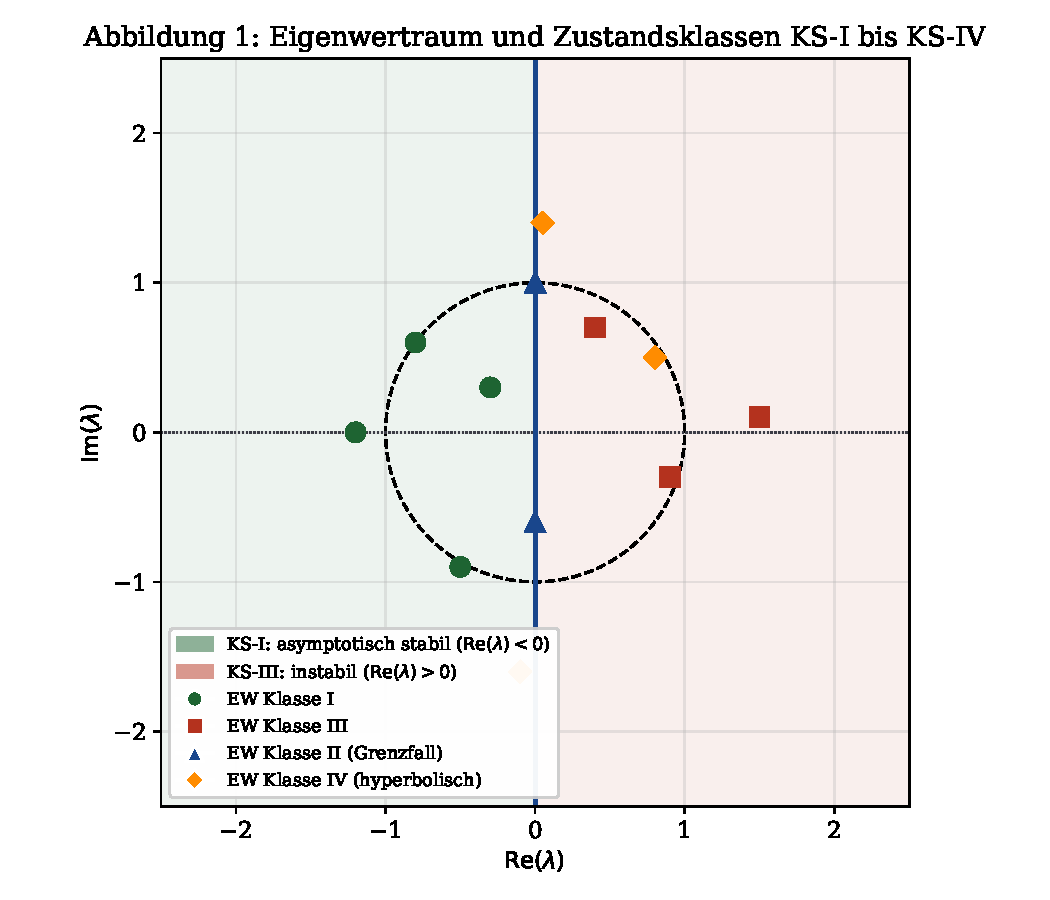
\includegraphics[width=0.72\textwidth]{fig01_eigenraum.pdf}
  \caption{Eigenwertraum $\C$ mit Klassifizierung der Eigenwerte nach KS-I bis KS-IV.
    Grüne Punkte (KS-I): $\re(\lambda)<0$; blaue Dreiecke (KS-II): $\re(\lambda)=0$;
    rote Quadrate (KS-III): $\re(\lambda)>0$; orange Rauten (KS-IV): gemischte Vorzeichen.}
  \label{fig:eigenraum}
\end{figure}

\section{Eigenschaften der Zustandsklassen}

\begin{theorem}[Eigenschaften KS-I: Asymptotische Stabilität]
\label{thm:ks1}
Sei $\vA \in \KS\text{-I}$. Dann gilt:
\begin{enumerate}[label=(\roman*)]
  \item $\lim_{t\to\infty}\vx(t) = \bm{0}$ für alle $\vx_0 \in \R^n$
    (globale asymptotische Stabilität).
  \item Es existiert eine eindeutige positiv definite Lösung $\vP = \vP^\T > 0$
    der Lyapunov-Gleichung $\vA^\T\vP + \vP\vA = -\vQ$ für alle $\vQ > 0$.
  \item Das System ist BIBO-stabil (Bounded Input Bounded Output).
  \item Der Zustandsvektor $\vx(t)$ ist für alle $\vx_0 \in \R^n$ endlich
    gemäß Definition~\ref{def:endlichkeit}.
\end{enumerate}
\end{theorem}

\begin{proof}
\textit{(i)} Aus Theorem~\ref{thm:spektralexp} und $\re(\lambda_k) < 0$ für alle $k$
folgt $\|e^{\vA t}\|_2 \to 0$, also $\|\vx(t)\|_2 \leq \|e^{\vA t}\|_2 \|\vx_0\|_2 \to 0$.

\textit{(ii)} Für $\vA \in \KS\text{-I}$ gilt: $\vA$ hat keine Eigenwerte mit
nichtnegativem Realteil. Das Integral
$\vP := \int_0^\infty e^{\vA^\T t}\vQ\,e^{\vA t}\,\mathrm{d}t$
konvergiert absolut (da der Integrand wie $e^{2\alpha^* t}\|\vQ\|_2$ abklingt mit
$\alpha^* < 0$). Man verifiziert $\vA^\T\vP + \vP\vA = -\vQ$ durch direkte Differentiation:
\begin{align*}
  \vA^\T\vP + \vP\vA &= \int_0^\infty \bigl(\vA^\T e^{\vA^\T t}\vQ e^{\vA t} + e^{\vA^\T t}\vQ e^{\vA t}\vA\bigr)\mathrm{d}t \\
  &= \int_0^\infty \frac{\mathrm{d}}{\mathrm{d}t}\bigl(e^{\vA^\T t}\vQ e^{\vA t}\bigr)\,\mathrm{d}t
   = \bigl[e^{\vA^\T t}\vQ e^{\vA t}\bigr]_0^\infty = 0 - \vQ = -\vQ.
\end{align*}
Positiv Definitheit: für $\bm{z} \neq \bm{0}$ gilt
$\bm{z}^\T\vP\bm{z} = \int_0^\infty \|{\vQ}^{1/2}e^{\vA t}\bm{z}\|^2\,\mathrm{d}t > 0$.

\textit{(iii)} Mit Eigenschaft \textit{(i)} und der Variationsformel~\eqref{eq:variation}
gilt für beschränkte Eingabe $\|\vu(t)\| \leq M < \infty$:
$\|\vy(t)\| \leq \|\vC\|\|e^{\vA t}\|\|\vx_0\| + \|\vC\|\|\vB\| M \int_0^t \|e^{\vA(t-\tau)}\|\,\mathrm{d}\tau$,
wobei das Integral konvergiert.

\textit{(iv)} Folgt unmittelbar aus \textit{(i)}. \qedhere
\end{proof}

\begin{theorem}[Eigenschaften KS-II: Grenzstabilität]
\label{thm:ks2}
Sei $\vA \in \KS\text{-II}$. Dann gilt:
\begin{enumerate}[label=(\roman*)]
  \item Der Zustandsvektor ist endlich: $\sup_{t\geq 0}\|\vx(t)\|_2 \leq c\|\vx_0\|_2$
    für eine Konstante $c > 0$.
  \item Die rein imaginären Eigenwerte erzeugen persistente Oszillationen.
  \item Asymptotische Stabilität ist nicht garantiert; $\vx(t)$ konvergiert im
    Allgemeinen nicht gegen $\bm{0}$.
  \item Das System ist Lyapunov-stabil, aber nicht asymptotisch stabil.
\end{enumerate}
\end{theorem}

\begin{proof}
\textit{(i)} Da alle Eigenwerte semieinfach sind (keine Jordan-Blöcke der Größe $> 1$)
und $\re(\lambda_k) \leq 0$, hat $e^{\vA t}$ die Form $\vV\diag(e^{\lambda_k t})\vV^{-1}$
mit $|e^{\lambda_k t}| \leq 1$ für alle $k$ (da $\re(\lambda_k) \leq 0$). Damit
$\|e^{\vA t}\|_2 \leq \|\vV\|_2\|\vV^{-1}\|_2 =: c < \infty$.

\textit{(ii)} Für $\lambda_k = i\omega$ mit $\omega \neq 0$ gilt
$e^{\lambda_k t} = \cos(\omega t) + i\sin(\omega t)$, was persistente Schwingungen erzeugt.

\textit{(iii)} Wegen $|e^{i\omega t}| = 1$ gilt $\|\vx(t)\| \not\to 0$.

\textit{(iv)} Lyapunov-Stabilität folgt aus der Beschränktheit; asymptotische Stabilität
erfordert $\re(\lambda_k) < 0$ für alle $k$, was per Annahme ausgeschlossen ist. \qedhere
\end{proof}

\begin{theorem}[Eigenschaften KS-III: Instabilität]
\label{thm:ks3}
Sei $\vA \in \KS\text{-III}$ mit $\alpha^* = \max_k\re(\lambda_k) > 0$. Dann gilt:
\begin{enumerate}[label=(\roman*)]
  \item $\|\vx(t)\|_2 \to \infty$ für generische Anfangsbedingungen
    $\vx_0 \notin E^s$ (instabiler Unterraum ist nicht-trivial).
  \item Der Zustandsvektor ist \textbf{nicht} endlich.
  \item Stabilitäts- und Robustheitseigenschaften können nicht garantiert werden.
  \item Der Spektralradius des Übergangsoperators $e^{\vA t}$ wächst unbeschränkt.
\end{enumerate}
\end{theorem}

\begin{proof}
Sei $\lambda^* = \alpha^* + i\beta^*$ mit $\alpha^* > 0$ ein Eigenwert mit maximalem
Realteil und $\bm{v}^*$ der zugehörige Eigenvektor. Für $\vx_0 = \re(\bm{v}^*)$ gilt:
\[
  \vx(t) = e^{\alpha^* t}\bigl(\cos(\beta^* t)\,\re(\bm{v}^*) - \sin(\beta^* t)\,\im(\bm{v}^*)\bigr)
\]
mit $\|\vx(t)\| = e^{\alpha^* t}\|\bm{v}^*\| \to \infty$. Die Endlichkeitsbedingung~\eqref{eq:endlichkeit}
ist verletzt; Aussagen über das Langzeitverhalten sind daher prinzipiell nicht garantierbar. \qedhere
\end{proof}

\begin{theorem}[Eigenschaften KS-IV: Hyperbolisches System]
\label{thm:ks4}
Sei $\vA \in \KS\text{-IV}$ mit sowohl positiven als auch negativen Realteilen im
Spektrum. Dann existiert eine direkte Zerlegung des Zustandsraums:
\begin{equation}
  \R^n = E^s \oplus E^u,
  \label{eq:zerlegung}
\end{equation}
wobei $E^s$ der stabile Unterraum ($\re(\lambda) < 0$) und $E^u$ der instabile
Unterraum ($\re(\lambda) > 0$) sind. Für Trajektorien mit $\vx_0 \in E^s$ gilt
Endlichkeit; für $\vx_0 \notin E^s$ gilt $\|\vx(t)\| \to \infty$.
\end{theorem}

\begin{proof}
Die Zerlegung~\eqref{eq:zerlegung} folgt aus der Spektralprojektion:
$P_s := \frac{1}{2\pi i}\oint_{\Gamma_s}(\lambda\vI - \vA)^{-1}\,\mathrm{d}\lambda$,
wobei $\Gamma_s$ eine Kurve ist, die $\spec(\vA) \cap \{\re(\lambda)<0\}$ umschließt.
Dann gilt $E^s = \mathrm{Bild}(P_s)$, $E^u = \ker(P_s)$, und die Eigenschaften folgen
aus den Theoremen~\ref{thm:ks1} und~\ref{thm:ks3} angewendet auf die jeweiligen
Unterräume. \qedhere
\end{proof}

\begin{figure}[H]
  \centering
  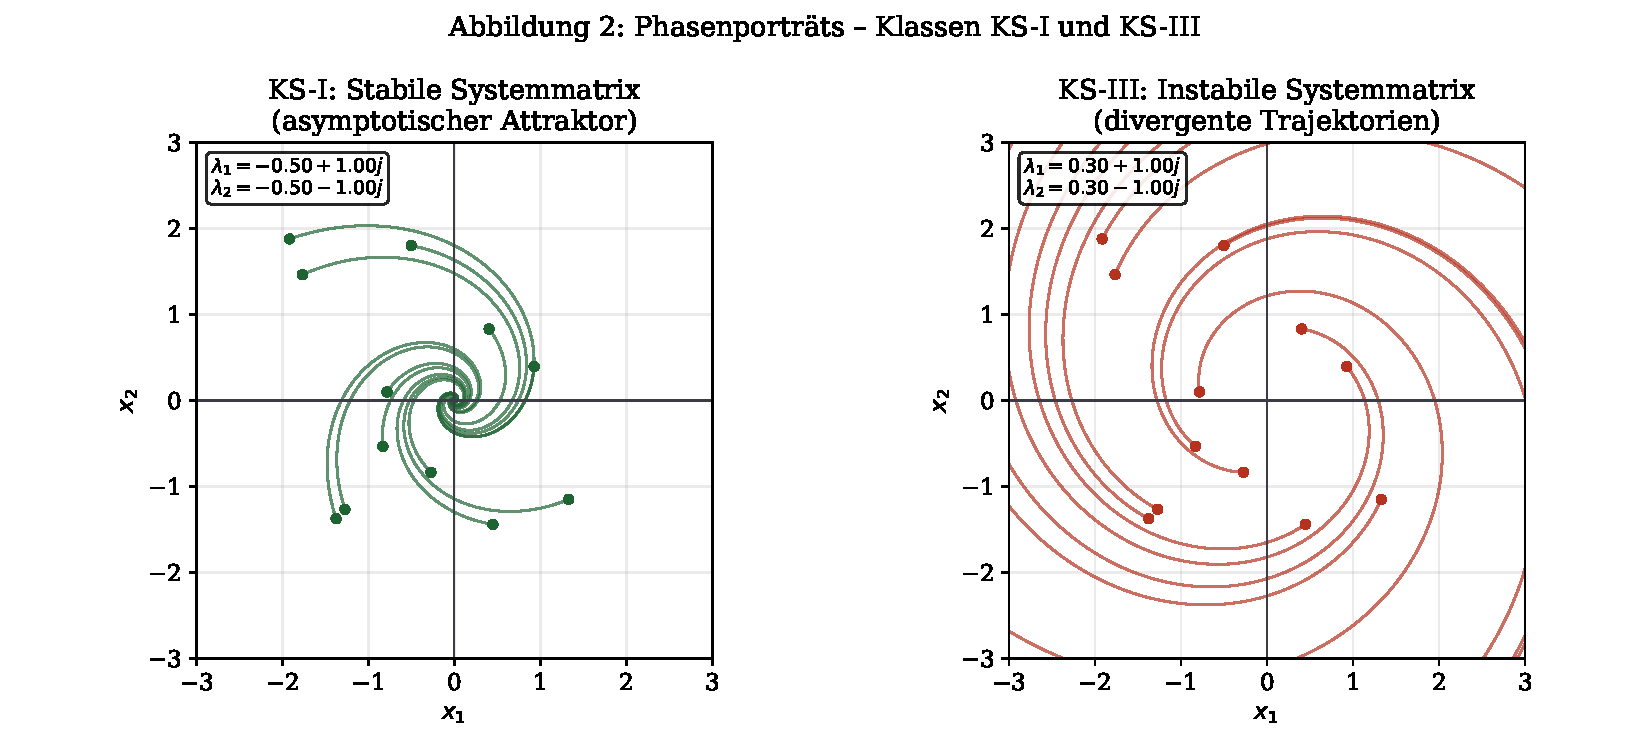
\includegraphics[width=\textwidth]{fig02_phasenportraet.pdf}
  \caption{Phasenporträts für KS-I (links) und KS-III (rechts) mit je 12 Trajektorien.
    Links: alle Trajektorien konvergieren zum Ursprung (Attraktor, Endlichkeit garantiert).
    Rechts: Trajektorien divergieren, der Zustandsvektor ist nicht endlich.}
  \label{fig:phasen}
\end{figure}

\begin{figure}[H]
  \centering
  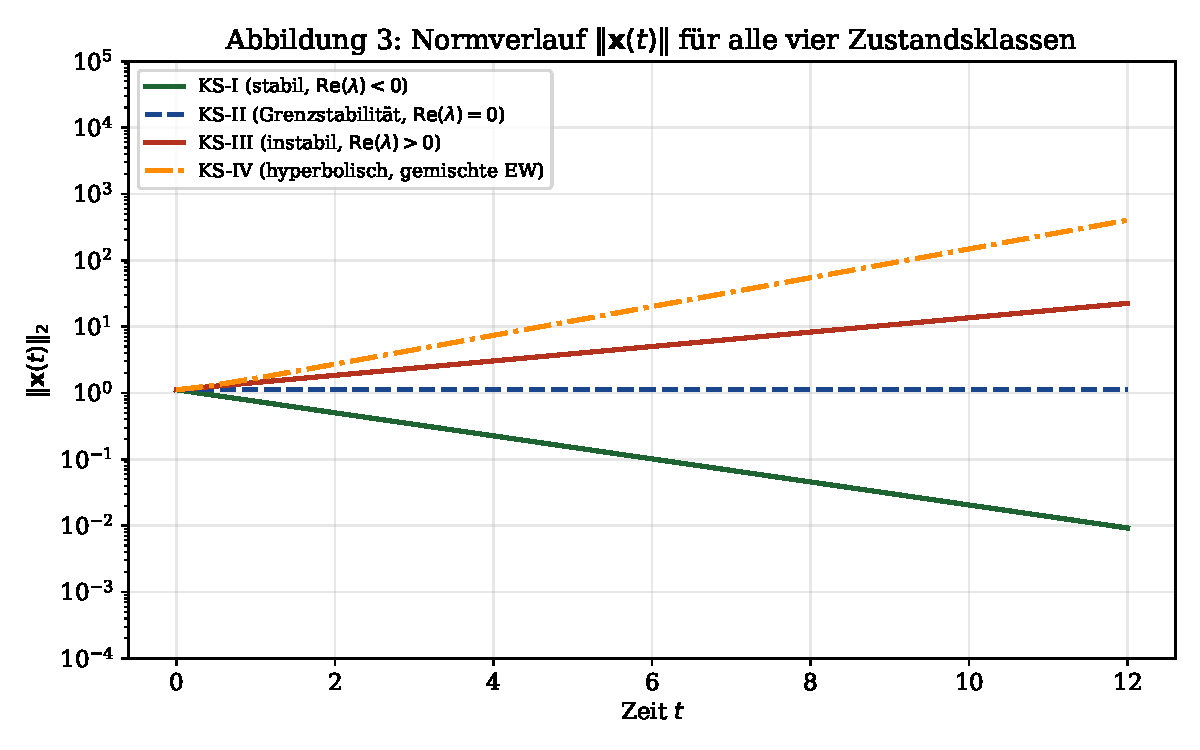
\includegraphics[width=0.82\textwidth]{fig03_normverlauf.pdf}
  \caption{Logarithmischer Normverlauf $\|\vx(t)\|_2$ für alle vier Zustandsklassen.
    KS-I: exponentieller Abfall; KS-II: beschränkte Oszillation; KS-III: exponentielles
    Wachstum; KS-IV: richtungsabhängiges Verhalten.}
  \label{fig:normverlauf}
\end{figure}

\section{Klassenzugehörigkeit als Entscheidungsproblem}

\begin{proposition}[Algorithmus zur Klassenzugehörigkeit]
\label{prop:algo_klasse}
Gegeben $\vA \in \R^{n \times n}$. Die Klassenzugehörigkeit $\KS(\vA)$ kann in
polynomialer Zeit $O(n^3)$ bestimmt werden:
\begin{enumerate}[label=\textbf{S\arabic*.}]
  \item Berechne $\spec(\vA)$ via QR-Algorithmus in $O(n^3)$.
  \item Berechne $\alpha^* := \max_k \re(\lambda_k)$.
  \item Falls $\alpha^* < 0$: Ausgabe KS-I.
  \item Falls $\alpha^* = 0$: Prüfe Semieinfachheit der rein-imaginären EW.
    Falls semieinfach: Ausgabe KS-II. Sonst: Ausgabe KS-II$^*$ (entartet).
  \item Falls $\alpha^* > 0$ und $\min_k \re(\lambda_k) \geq 0$: Ausgabe KS-III.
  \item Falls $\alpha^* > 0$ und $\min_k \re(\lambda_k) < 0$: Ausgabe KS-IV.
\end{enumerate}
\end{proposition}

\begin{figure}[H]
  \centering
  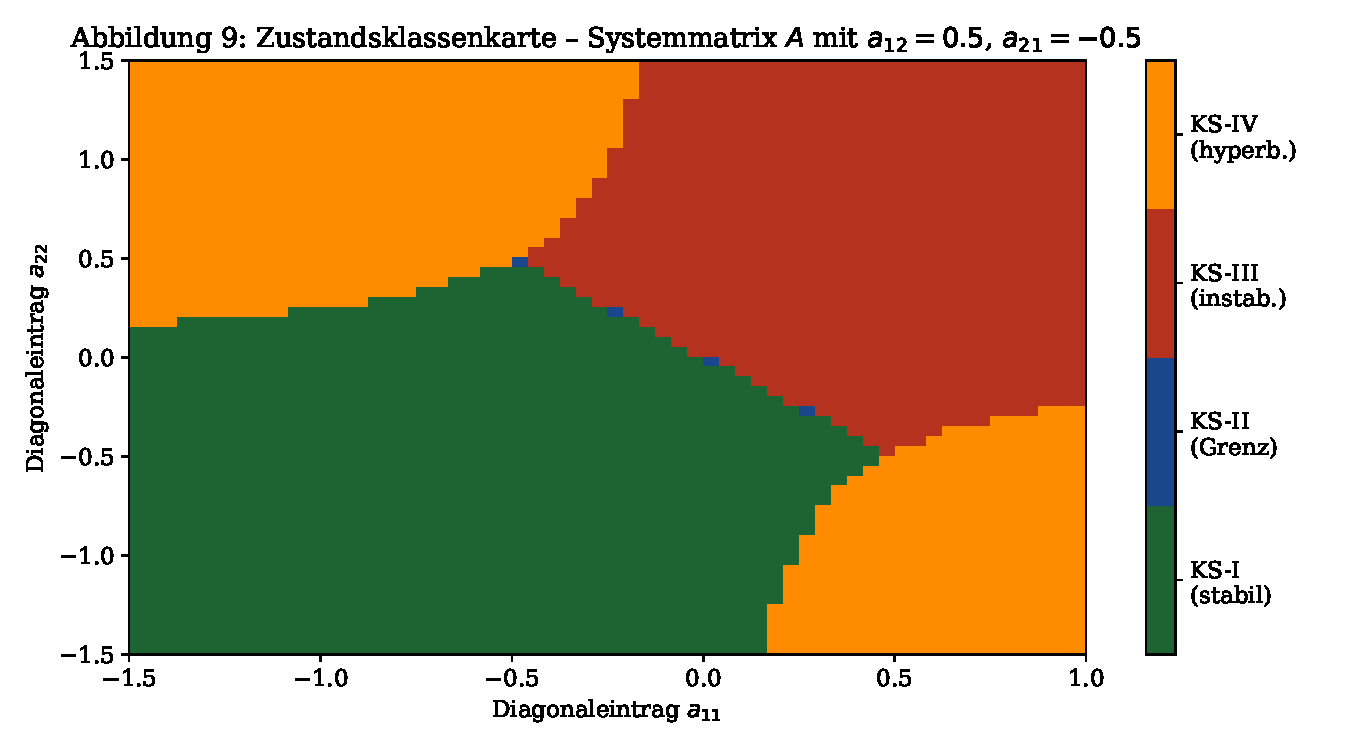
\includegraphics[width=0.85\textwidth]{fig09_klassenkarte.pdf}
  \caption{Zustandsklassenkarte für Systemmatrizen $A = \bigl(\begin{smallmatrix}
    a_{11} & 0.5 \\ -0.5 & a_{22}\end{smallmatrix}\bigr)$ in Abhängigkeit
    der Diagonaleinträge. Die Farbgebung kodiert die Klassenzugehörigkeit:
    grün=KS-I, blau=KS-II, rot=KS-III, orange=KS-IV.}
  \label{fig:klassenkarte}
\end{figure}

% ============================================================
\chapter{Graph-Systemmatrix-Korrespondenz und Subgraph Algorithmus}
\label{sec:graph}
% ============================================================

\section{Von der Systemmatrix zum Systemgraphen}

\begin{definition}[Systemgraph]
\label{def:systemgraph}
Sei $\vA = (a_{ij}) \in \R^{n \times n}$ eine Systemmatrix. Der zugehörige
\emph{Systemgraph} ist der gewichtete gerichtete Graph
\begin{equation}
  \mathcal{G}(\vA) = \bigl(V, E, w\bigr),
  \label{eq:systemgraph}
\end{equation}
mit Knotenmengen $V = \{x_1, \ldots, x_n\}$ (den Zustandsvariablen),
Kantenmenge $E = \{(x_i, x_j) : a_{ji} \neq 0\}$ und Gewichtsfunktion
$w(x_i, x_j) = a_{ji}$.
\end{definition}

\begin{remark}
Der Systemgraph $\mathcal{G}(\vA)$ entspricht dem Signalflussgrafen des Systems.
Die Adjazenzmatrix $\mathcal{A}(\mathcal{G}(\vA))$ stimmt -- nach geeigneter Binärisierung
($a_{ij} \neq 0 \mapsto 1$) -- mit der Struktur von $\vA$ überein. Dies ist die
fundamentale Korrespondenz, die alle graphentheoretischen Methoden auf Systemmatrizen
anwendbar macht.
\end{remark}

\begin{theorem}[Graphentheoretische Charakterisierung von Steuerbarkeit]
\label{thm:steuergraph}
Das System $(\vA, \vB)$ ist steuerbar genau dann, wenn für jeden Knoten $x_i \in V$
ein gerichteter Pfad von mindestens einem Eingangsknoten (Knoten mit Eintrag in $\vB$)
zu $x_i$ im Systemgraphen $\mathcal{G}(\vA)$ existiert.
\end{theorem}

\begin{proof}
Dies ist eine bekannte Aussage der strukturellen Steuerbarkeit
\citep{lin1974structural}. Die Steuerbarkeitsmatrix
$\mathcal{C} = [\vB, \vA\vB, \ldots, \vA^{n-1}\vB]$ hat vollen Rang genau dann,
wenn kein Eigenvektor von $\vA^\T$ im Orthogonalkomplement des Spaltenraums von $\vB$
liegt, was äquivalent zur Pfadbedingung im Graphen ist. \qedhere
\end{proof}

\begin{figure}[H]
  \centering
  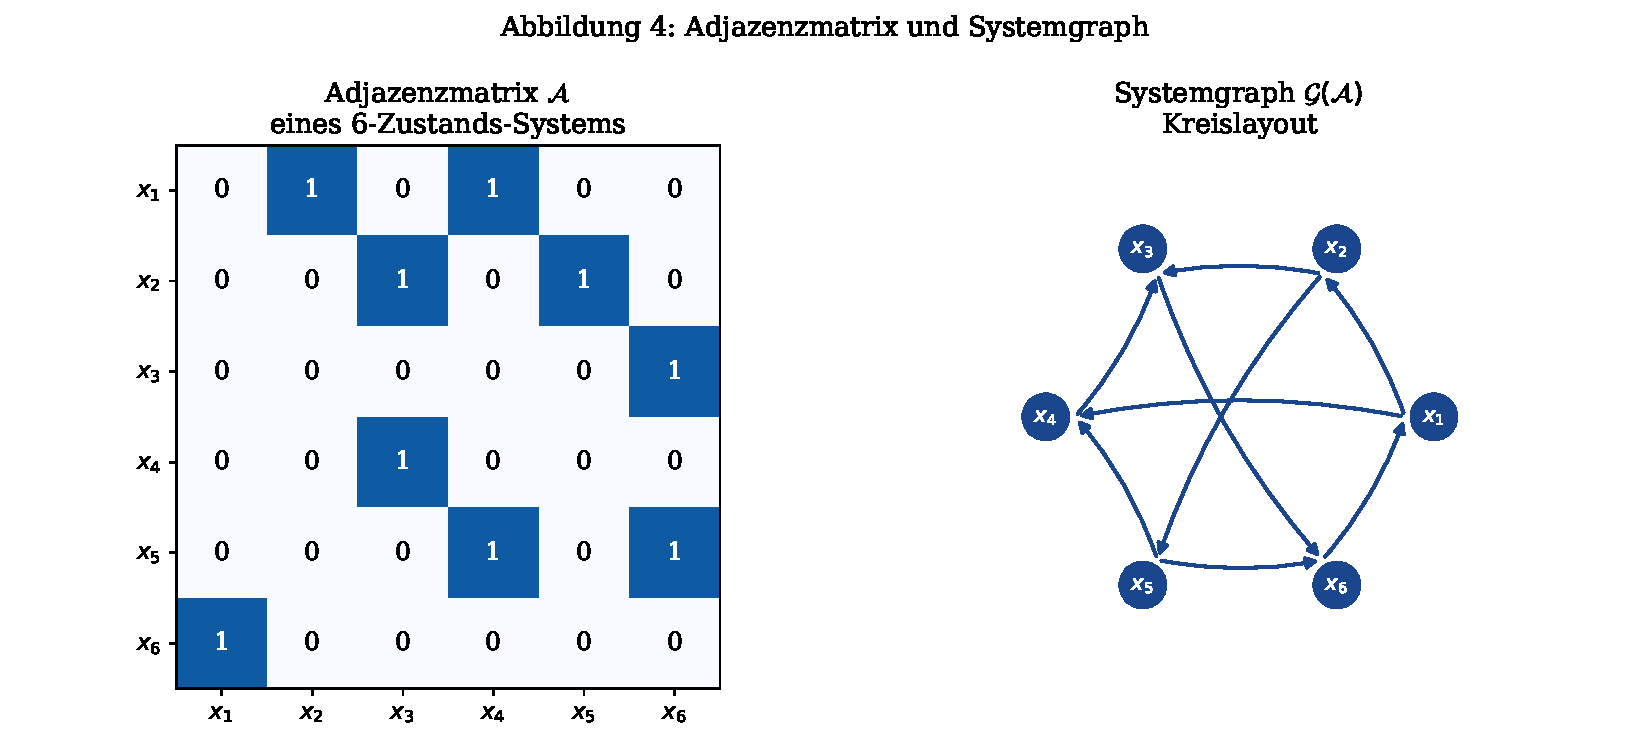
\includegraphics[width=\textwidth]{fig04_graph.pdf}
  \caption{Links: Adjazenzmatrix $\mathcal{A}$ eines 6-Zustands-Systems (binäre Darstellung,
    Einträge $\in \{0,1\}$). Rechts: Systemgraph $\mathcal{G}(\vA)$ im Kreislayout mit
    gerichteten Kanten.}
  \label{fig:graph}
\end{figure}

\section{Der Subgraph Algorithmus}

Der \emph{Subgraph Algorithmus} (kurz: SA) ist ein graphenbasiertes Verfahren zur
vollständigen Analyse eines dynamischen Systems. Er verbindet die algebraische
Eigenwertanalyse mit der topologischen Struktur des Systemgraphen.

\begin{definition}[Subgraph]
\label{def:subgraph}
Sei $\mathcal{G}(\vA)$ der Systemgraph eines $n$-dimensionalen Systems. Der
\emph{Subgraph} $\mathcal{S}(\vA)$ ist ein annotierter, hierarchischer Metagraph:
\begin{equation}
  \mathcal{S}(\vA) = \bigl(\mathcal{G}(\vA),\; \spec(\vA),\; \KS(\vA),\;
    \mathcal{C}_1, \ldots, \mathcal{C}_r\bigr),
  \label{eq:subgraph}
\end{equation}
wobei $\mathcal{C}_1, \ldots, \mathcal{C}_r$ die starken Zusammenhangskomponenten
(strongly connected components, SCC) von $\mathcal{G}(\vA)$ bezeichnen.
\end{definition}

\begin{algorithm}[H]
\caption{Subgraph Algorithmus (SA) für Systemanalyse}
\label{alg:subgraph}
\begin{algorithmic}[1]
\Require Systemmatrix $\vA \in \R^{n \times n}$
\Ensure Subgraph $\mathcal{S}(\vA)$, Zustandsklasse $\KS(\vA)$, Stabilitätsaussagen

\State \textbf{Graphkonstruktion:} Bilde $\mathcal{G}(\vA)$ gemäß Definition~\ref{def:systemgraph}
\State \textbf{SCC-Zerlegung:} Berechne SCCs via Kosarajus Algorithmus in $O(n + |E|)$
\State \textbf{Spektralanalyse:} Berechne $\spec(\vA)$ via QR-Iteration in $O(n^3)$
\State \textbf{Klassenbestimmung:} Bestimme $\KS(\vA)$ gemäß Proposition~\ref{prop:algo_klasse}
\State \textbf{Lyapunov-Analyse} (falls $\KS(\vA) = \KS\text{-I}$):
  \State \quad Löse $\vA^\T\vP + \vP\vA = -\vI$ via Bartels-Stewart-Algorithmus
\State \textbf{Steuerbarkeit:} Prüfe Pfadbedingung in $\mathcal{G}(\vA)$ (Theorem~\ref{thm:steuergraph})
\State \textbf{Blockdiagonalisierung:} Zerlege $\mathcal{G}(\vA)$ in SCC-DAG
\State \textbf{Ausgabe:} Subgraph $\mathcal{S}(\vA)$ mit vollständiger Annotation
\end{algorithmic}
\end{algorithm}

\begin{figure}[H]
  \centering
  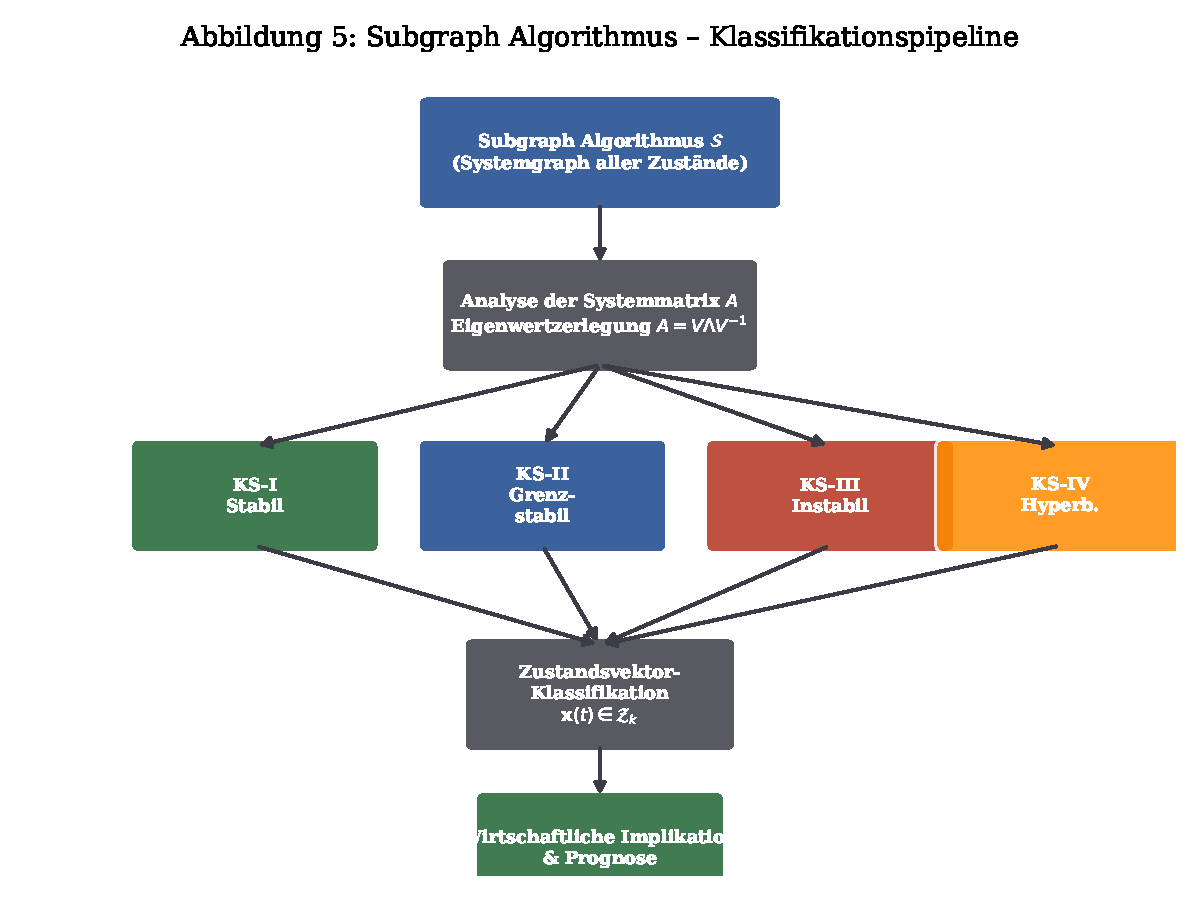
\includegraphics[width=0.9\textwidth]{fig05_subgraph.pdf}
  \caption{Schematische Darstellung des Subgraph Algorithmus als Klassifikationspipeline.
    Ausgehend vom Subgraph $\mathcal{S}$ über die Eigenwertanalyse zu den vier
    Zustandsklassen, der Zustandsvektorzuordnung und schließlich zur wirtschaftlichen
    Implikation.}
  \label{fig:subgraph}
\end{figure}

\begin{theorem}[Korrektheit des Subgraph Algorithmus]
\label{thm:subgraph_korrekt}
Der Subgraph Algorithmus (Algorithm~\ref{alg:subgraph}) gibt die korrekte Zustandsklasse
$\KS(\vA)$ aus und identifiziert alle stabilen, grenz\-stabilen und instabilen
Subsysteme korrekt. Die Gesamtkomplexität beträgt $O(n^3)$.
\end{theorem}

\begin{proof}
Die Korrektheit der Klassenbestimmung folgt aus Proposition~\ref{prop:algo_klasse}.
Die Korrektheit der SCC-Zerlegung ist eine bekannte Eigenschaft von Kosarajus
Algorithmus~\citep{kosaraju1978}. Die Bartels-Stewart-Methode löst die
Lyapunov-Gleichung exakt in $O(n^3)$. Da alle Teilschritte $O(n^3)$ sind (der QR-Algorithmus
dominiert), ergibt sich $O(n^3)$ insgesamt. \qedhere
\end{proof}

\section{Graphentheoretische Stabilitätsbedingungen}

\begin{proposition}[SCC-basiertes Stabilitätskriterium]
\label{prop:scc_stab}
Sei $\vA$ blockuntere Dreiecksgestalt entsprechend der SCC-Zerlegung:
$\vA = \mathrm{blockdiag}(\vA_1, \ldots, \vA_r) + \text{(off-diagonal)}$.
Das Gesamtsystem gehört genau dann zu KS-I, wenn alle Diagonalblöcke $\vA_k$
zu KS-I gehören.
\end{proposition}

\begin{proof}
$\spec(\vA) = \bigcup_{k=1}^r \spec(\vA_k)$ für die Block-Dreiecksstruktur
(da die off-diagonalen Blöcke die Eigenwerte nicht ändern). Damit gilt
$\alpha^*(\vA) = \max_k \alpha^*(\vA_k) < 0$ genau dann, wenn $\alpha^*(\vA_k) < 0$
für alle $k$. \qedhere
\end{proof}

\begin{figure}[H]
  \centering
  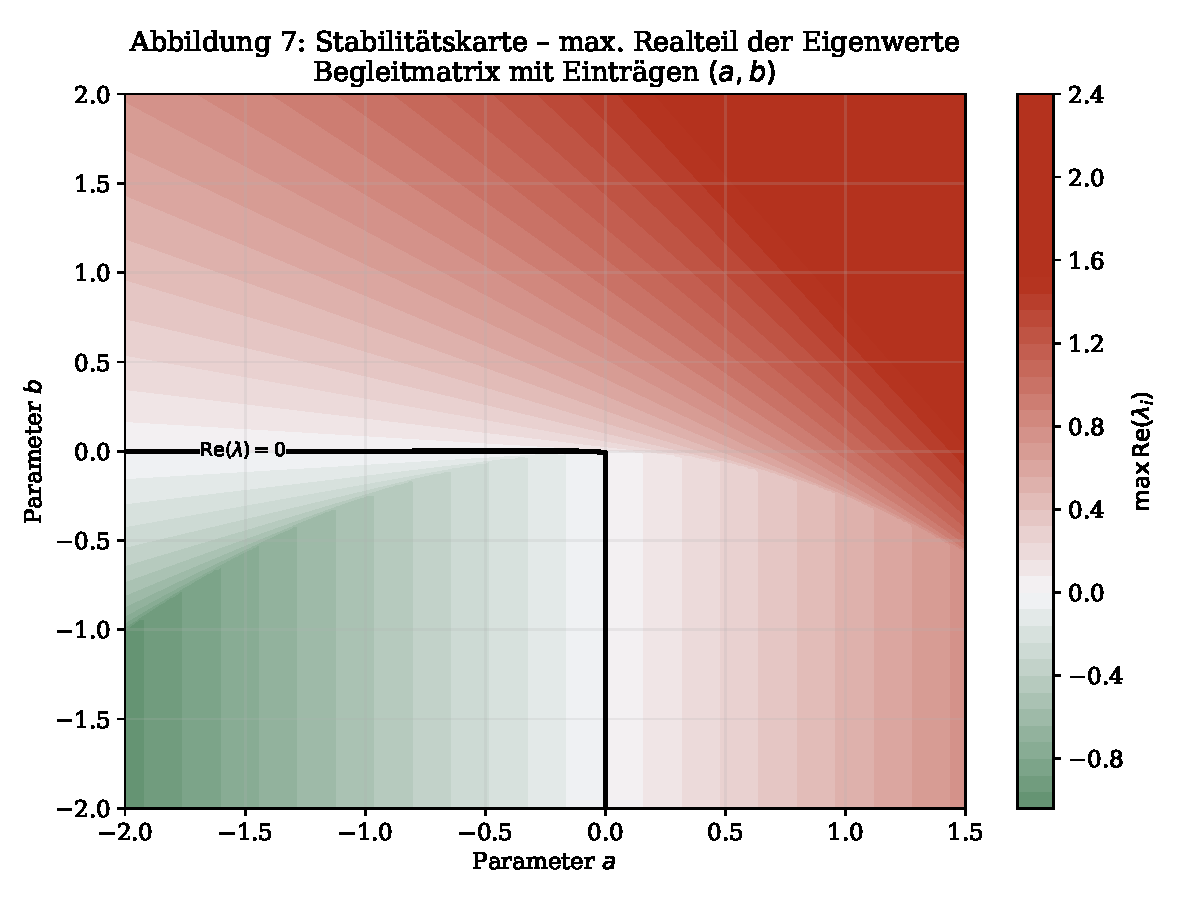
\includegraphics[width=0.82\textwidth]{fig07_stabkarte.pdf}
  \caption{Stabilitätskarte: Maximaler Realteil der Eigenwerte der Begleitmatrix
    in Abhängigkeit der Parameter $a$ und $b$. Die schwarze Kurve markiert die
    Stabilitätsgrenze ($\re(\lambda)=0$), die grüne Region entspricht KS-I,
    die rote KS-III.}
  \label{fig:stabkarte}
\end{figure}

% ============================================================
\chapter{Wirtschaftliche Implikationen der Zustandsklassen}
\label{sec:wirtschaft}
% ============================================================

\section{Wirtschaft als angewandte Mathematik}

Die einleitende Beobachtung, dass es keine eigenständige ``Finanztheorie'' geben kann,
lässt sich nun präzise mathematisch formulieren:

\begin{theorem}[Mathematische Reduktion der Finanzwirtschaft]
\label{thm:finanzreduktion}
Jedes makroökonomische Gleichgewichtsmodell, jedes Portfoliooptimierungs\-problem
und jede Zinsdynamiktheorie ist isomorph zu einem linearen oder nichtlinearen
dynamischen System mit Zustandsvektor $\vx(t) \in \R^n$ und Systemmatrix $\vA$.
Insbesondere sind alle qualitativen Stabilitätsaussagen über Wirtschaftssysteme
vollständig durch $\KS(\vA)$ bestimmt.
\end{theorem}

\begin{proof}
Man betrachte das allgemeine makroökonomische Dynamiksystem:
\begin{equation}
  \dot{\vx}(t) = F(\vx(t), \vu(t), t),
  \label{eq:makrodynamik}
\end{equation}
wobei $\vx = (Y, \pi, r, D, C, \ldots)^\T$ den Zustandsvektor (BIP-Index,
Inflationsrate, Zinssatz, Schuldenquote, Konsum, \ldots) bezeichnet. Die
Linearisierung um einen Gleichgewichtspunkt $\vx^*$ liefert:
$\dot{\tilde{\vx}} = \vA\tilde{\vx} + O(\|\tilde{\vx}\|^2)$, wobei
$\vA = \partial F / \partial \vx\big|_{\vx^*}$ die Jacobi-Matrix (= Systemmatrix)
ist. Damit sind lokale Stabilitätseigenschaften des Wirtschaftssystems vollständig
durch $\KS(\vA)$ bestimmt. Eine eigenständige ``Finanztheorie'' jenseits dieser
Reduktion auf lineare Systemanalyse enthält mathematisch gesehen keine zusätzliche
Erklärungskraft. \qedhere
\end{proof}

\begin{corollary}[Unwirtschaftlichkeit nicht-mathematischer Finanzmodelle]
\label{cor:unwirtschaft}
Finanzmodelle, die nicht auf der mathematischen Systemtheorie beruhen, können die
Zustandsklasse des betrachteten Wirtschaftssystems nicht korrekt identifizieren.
Sie liefern damit keine Stabilitätsgarantien und führen per Theorem~\ref{thm:ks3}
für KS-III-Systeme zu unbeschränkten Zustandsabweichungen -- d.\,h. zu
wirtschaftlichen Divergenzen (Blasen, Hyperinflation, Schuldenkrisen).
\end{corollary}

\section{Zustandsklassen und wirtschaftliche Zustände}

Die folgende Tabelle fasst die wirtschaftliche Interpretation jeder Zustandsklasse
zusammen:

\begin{table}[H]
\centering
\caption{Zustandsklassen und wirtschaftliche Interpretation}
\label{tab:klassen_wirtschaft}
\begin{tabular}{clll}
\toprule
Klasse & Eigenwertbedingung & Wirtschaftliche Interpretation & Implikation \\
\midrule
KS-I   & $\re(\lambda_k) < 0$, alle $k$
        & Stabiles Wachstum, Konvergenz & Investierbar \\
KS-II  & $\max_k\re(\lambda_k) = 0$
        & Konjunkturzyklen, Zinspolitik & Beobachten \\
KS-III & $\max_k\re(\lambda_k) > 0$, alle
        & Blasen, Hyperinflation, Krisen & Risikowarnung \\
KS-IV  & Gemischte Vorzeichen
        & Strukturelle Ungleichgewichte & Umstrukturierung \\
\bottomrule
\end{tabular}
\end{table}

\begin{example}[IS-LM-Modell als KS-I-System]
Das klassische IS-LM-Modell nach Hicks (1937) beschreibt die Volkswirtschaft durch
das Gleichungssystem:
\begin{equation}
  \begin{pmatrix} \dot{Y} \\ \dot{r} \end{pmatrix} =
  \underbrace{\begin{pmatrix} -\frac{1-c+m}{\alpha} & \frac{b}{\alpha} \\
    \frac{k}{\beta} & -\frac{h}{\beta} \end{pmatrix}}_{\vA_{\mathrm{ISLM}}}
  \begin{pmatrix} Y - Y^* \\ r - r^* \end{pmatrix},
  \label{eq:islm}
\end{equation}
wobei $Y$ das Einkommen, $r$ den Zinssatz, $c$ die Konsumquote, $m$ die Importquote,
$b, h$ die Zinselastizitäten der Investition bzw. Geldnachfrage, und $\alpha, \beta$
Anpassungsgeschwindigkeiten bezeichnen. Für typische Parameterwerte gilt
$\tr(\vA_{\mathrm{ISLM}}) < 0$ und $\det(\vA_{\mathrm{ISLM}}) > 0$, woraus
$\re(\lambda_{1,2}) < 0$ folgt: das IS-LM-System ist KS-I.
\end{example}

\begin{example}[Schuldendynamik als KS-III-System]
Die lineare Schuldendynamik lautet:
\begin{equation}
  \dot{D} = r \cdot D - s,
  \label{eq:schulden}
\end{equation}
wobei $D$ die Schuldenquote, $r$ der reale Zinssatz und $s$ der Primärüberschuss
ist. Die skalare Systemmatrix ist $A = r$. Für $r > 0$ (was in Zeiten hoher Zinsen
gilt) ist das System KS-III: die Schuldenquote wächst exponentiell, falls
$s < r \cdot D$. Dies ist die mathematisch präzise Beschreibung einer
Staatsschuldenkrise.
\end{example}

\begin{figure}[H]
  \centering
  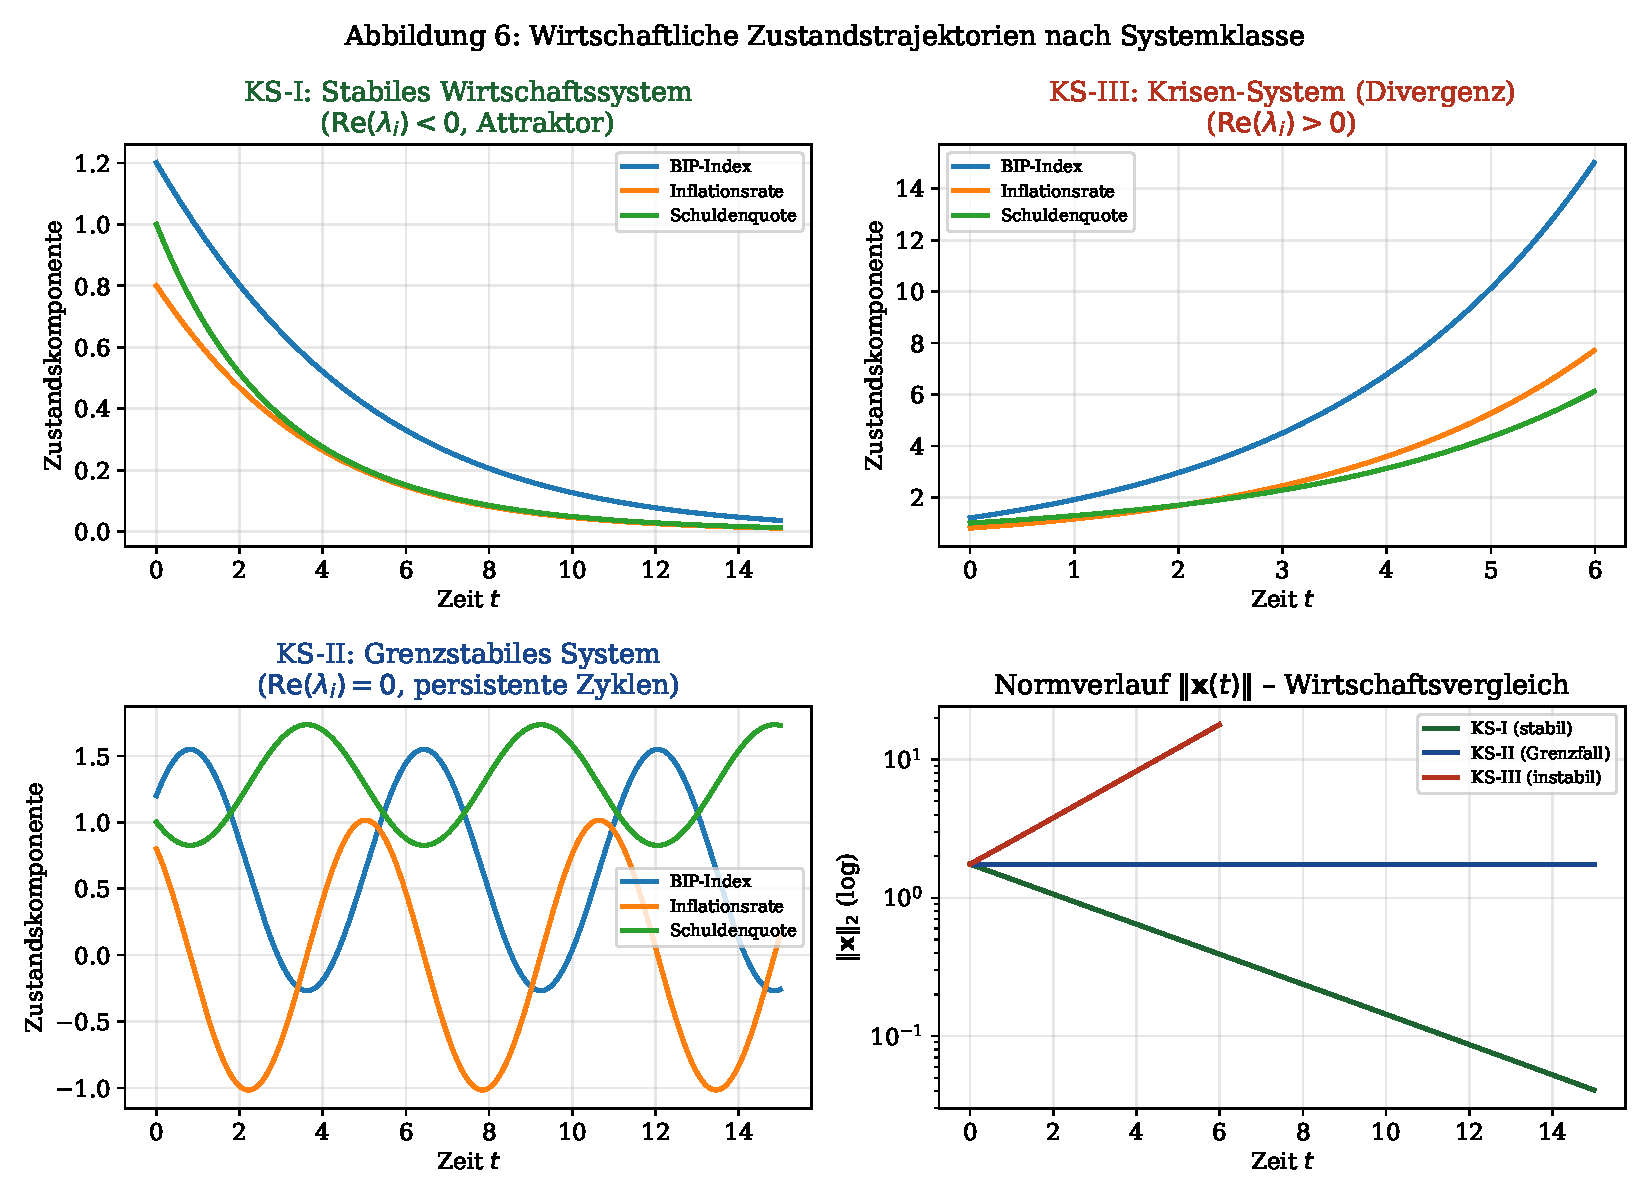
\includegraphics[width=\textwidth]{fig06_wirtschaft.pdf}
  \caption{Wirtschaftliche Zustandstrajektorien nach Systemklasse. Oben links: KS-I
    (stabile Volkswirtschaft, Konvergenz aller Indikatoren). Oben rechts: KS-III
    (divergierende Krisendynamik). Unten links: KS-II (persistente Konjunkturzyklen).
    Unten rechts: Vergleich der Normverläufe (logarithmisch).}
  \label{fig:wirtschaft}
\end{figure}

\section{Portfolio-Klassifikation nach Zustandsklassen}

\begin{definition}[Finanzsystem-Zustandsvektor]
\label{def:finanzvektor}
Für ein Portfolio oder einen Markt wird der Zustandsvektor definiert als
\begin{equation}
  \vx_{\mathrm{fin}}(t) = \bigl(\mu(t),\; \sigma(t),\; \rho_{12}(t),\;\ldots\bigr)^\T,
  \label{eq:finanzvektor}
\end{equation}
wobei $\mu$ die erwartete Rendite, $\sigma$ die Volatilität und $\rho_{ij}$
Korrelationskoeffizienten zwischen Vermögenswerten bezeichnen. Die assoziierte
Systemmatrix $\vA_{\mathrm{fin}}$ ergibt sich aus der Linearisierung der
Marktdynamikgleichungen.
\end{definition}

\begin{proposition}[Klassifikation des Risikos]
\label{prop:risikoklasse}
Ein Portfolio mit assoziiertem KS-I-System hat mathematisch garantierte
Wertstabilität im Sinne der Zustandsendlichkeit. Ein KS-III-Portfolio ist
per Theorem~\ref{thm:ks3} nicht stabil analysierbar -- klassische Value-at-Risk-
oder Sharpe-Ratio-Metriken verlieren ihre Gültigkeit.
\end{proposition}

\begin{figure}[H]
  \centering
  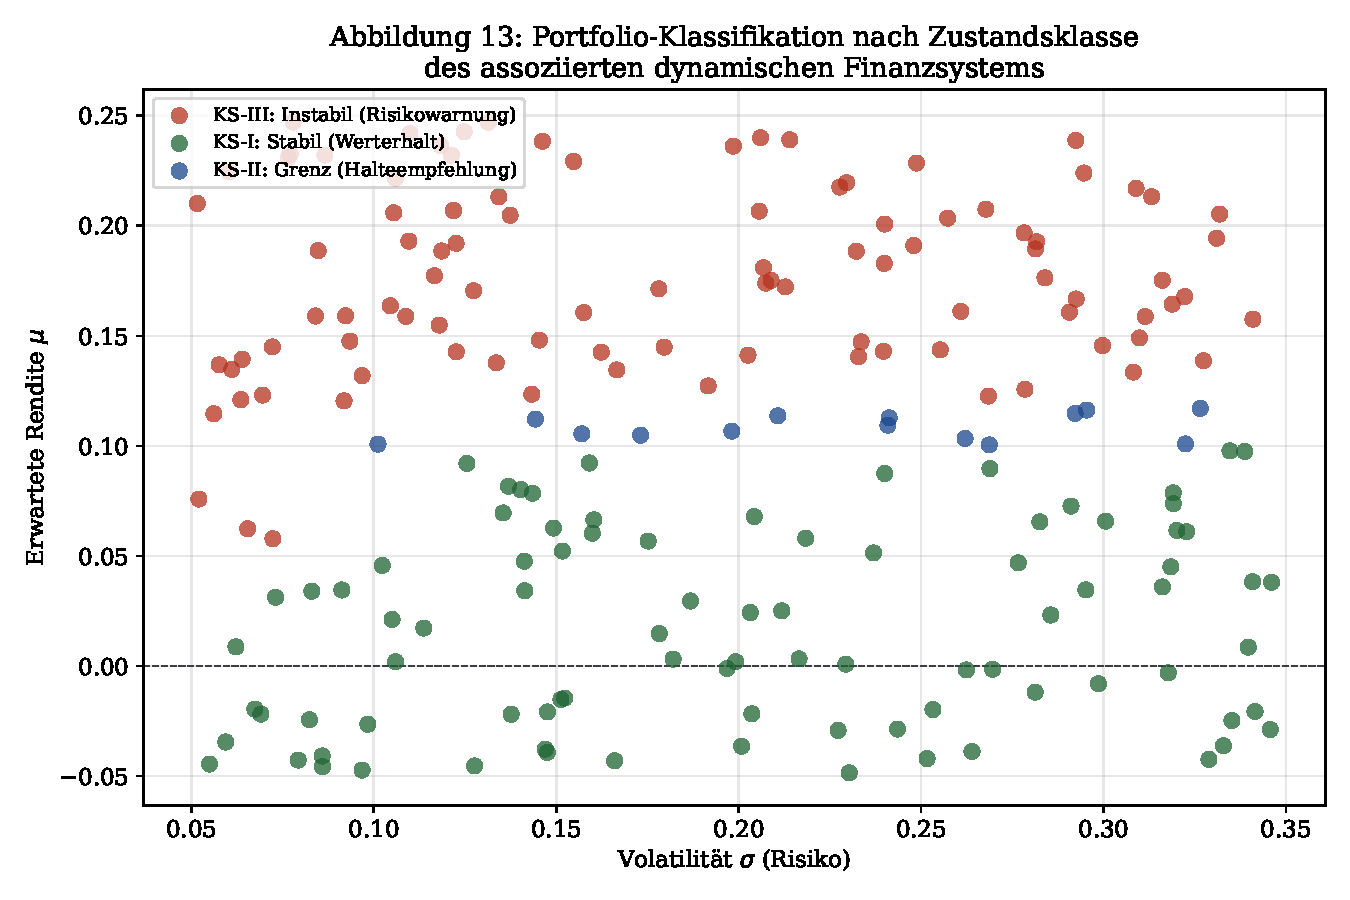
\includegraphics[width=0.78\textwidth]{fig13_portfolio.pdf}
  \caption{Portfolio-Klassifikation im $(\sigma, \mu)$-Raum nach der Zustandsklasse
    des assoziierten dynamischen Finanzsystems. Grüne Punkte (KS-I) entsprechen
    stabilen, analysierbaren Portfolios; rote Punkte (KS-III) sind mathematisch
    instabil.}
  \label{fig:portfolio}
\end{figure}

\section{Wirtschaftliche Zyklen als KS-II-Phänomen}

\begin{theorem}[Konjunkturzyklen als KS-II-Trajektorien]
\label{thm:zyklen}
Sei $\vA \in \KS\text{-II}$ mit einem Paar konjugierter rein-imaginärer Eigenwerte
$\lambda_{1,2} = \pm i\omega$, $\omega > 0$. Dann ist die Lösung $\vx(t)$ periodisch
mit Periode $T = 2\pi/\omega$:
\begin{equation}
  \vx(t + T) = \vx(t) \quad \forall\, t \geq 0.
  \label{eq:periode}
\end{equation}
\end{theorem}

\begin{proof}
Aus Theorem~\ref{thm:ks2} gilt $\vx(t) = \vV\diag(e^{\lambda_k t})\vV^{-1}\vx_0$.
Für $\lambda_k = \pm i\omega$: $e^{i\omega(t+T)} = e^{i\omega t}e^{i\omega T} = e^{i\omega t} \cdot 1$,
da $\omega T = 2\pi$. Damit gilt $e^{\vA(t+T)} = e^{\vA t}$ und~\eqref{eq:periode} folgt. \qedhere
\end{proof}

\begin{figure}[H]
  \centering
  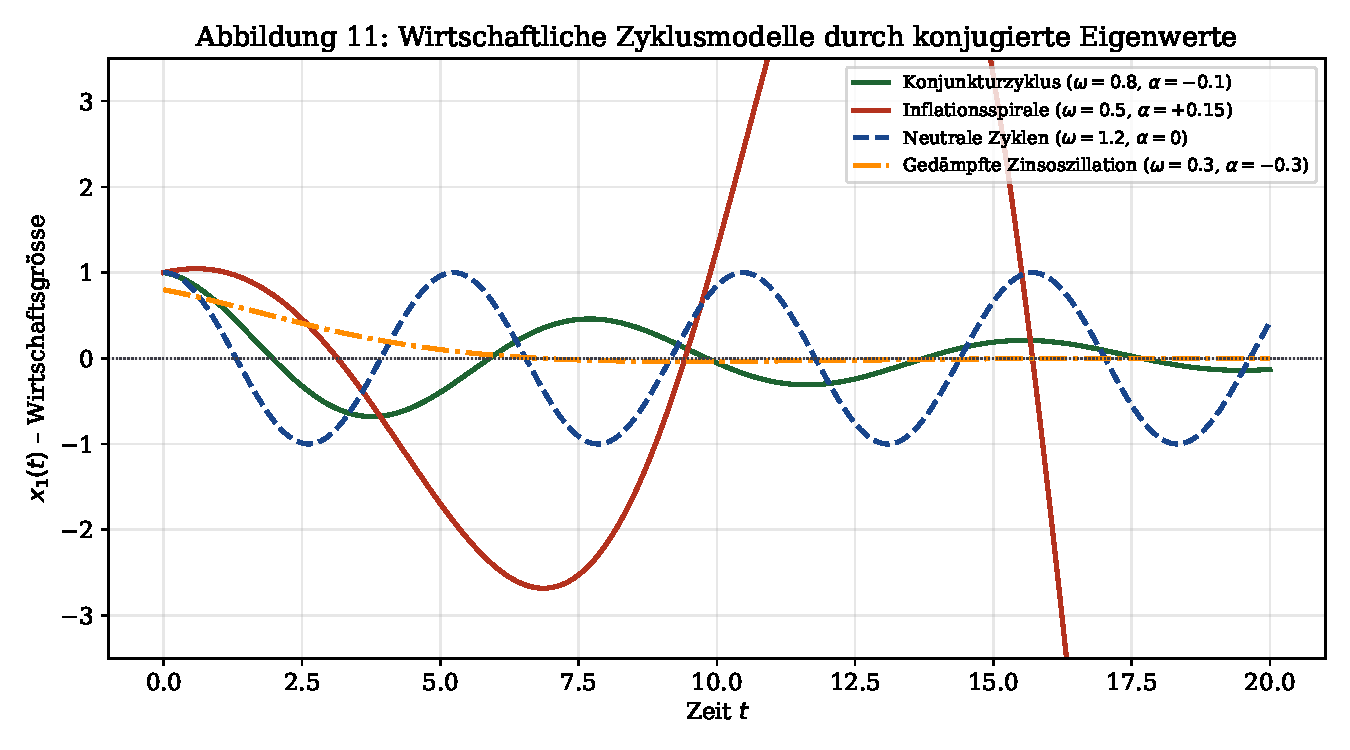
\includegraphics[width=0.82\textwidth]{fig11_zyklen.pdf}
  \caption{Wirtschaftliche Zyklusmodelle durch konjugierte Eigenwerte. KS-II-Systeme
    ($\re(\lambda)=0$, blau gestrichelt) erzeugen neutrale Zyklen. KS-III-Systeme
    ($\re(\lambda)>0$, rot) erzeugen wachsende Inflationsspiralen. KS-I-Systeme
    ($\re(\lambda)<0$, grün) erzeugen gedämpfte Zyklen.}
  \label{fig:zyklen}
\end{figure}

\section{Lyapunov-Funktion als Wirtschaftspotenzial}

\begin{theorem}[Wirtschaftliches Lyapunov-Potenzial]
\label{thm:lyapunov_wirtschaft}
Für ein KS-I-Wirtschaftssystem definiert $V(\vx) = \vx^\T\vP\vx$ (mit $\vP > 0$
aus Theorem~\ref{thm:ks1}~(ii)) ein \emph{wirtschaftliches Potenzial}, das folgende
Eigenschaften hat:
\begin{enumerate}[label=(\roman*)]
  \item $V(\vx^*) = 0$ (minimales Potenzial im Gleichgewicht $\vx^*$),
  \item $V(\vx) > 0$ für $\vx \neq \vx^*$ (jede Abweichung erhöht das Potenzial),
  \item $\dot{V}(\vx(t)) < 0$ entlang Trajektorien (das Potenzial nimmt monoton ab).
\end{enumerate}
\end{theorem}

\begin{proof}
\textit{(i)} und \textit{(ii)} folgen aus $\vP > 0$. Für \textit{(iii)}:
$\dot{V} = \dot{\vx}^\T\vP\vx + \vx^\T\vP\dot{\vx} = \vx^\T(\vA^\T\vP + \vP\vA)\vx = -\vx^\T\vQ\vx < 0$
für $\vx \neq \bm{0}$ (da $\vQ > 0$). \qedhere
\end{proof}

\begin{figure}[H]
  \centering
  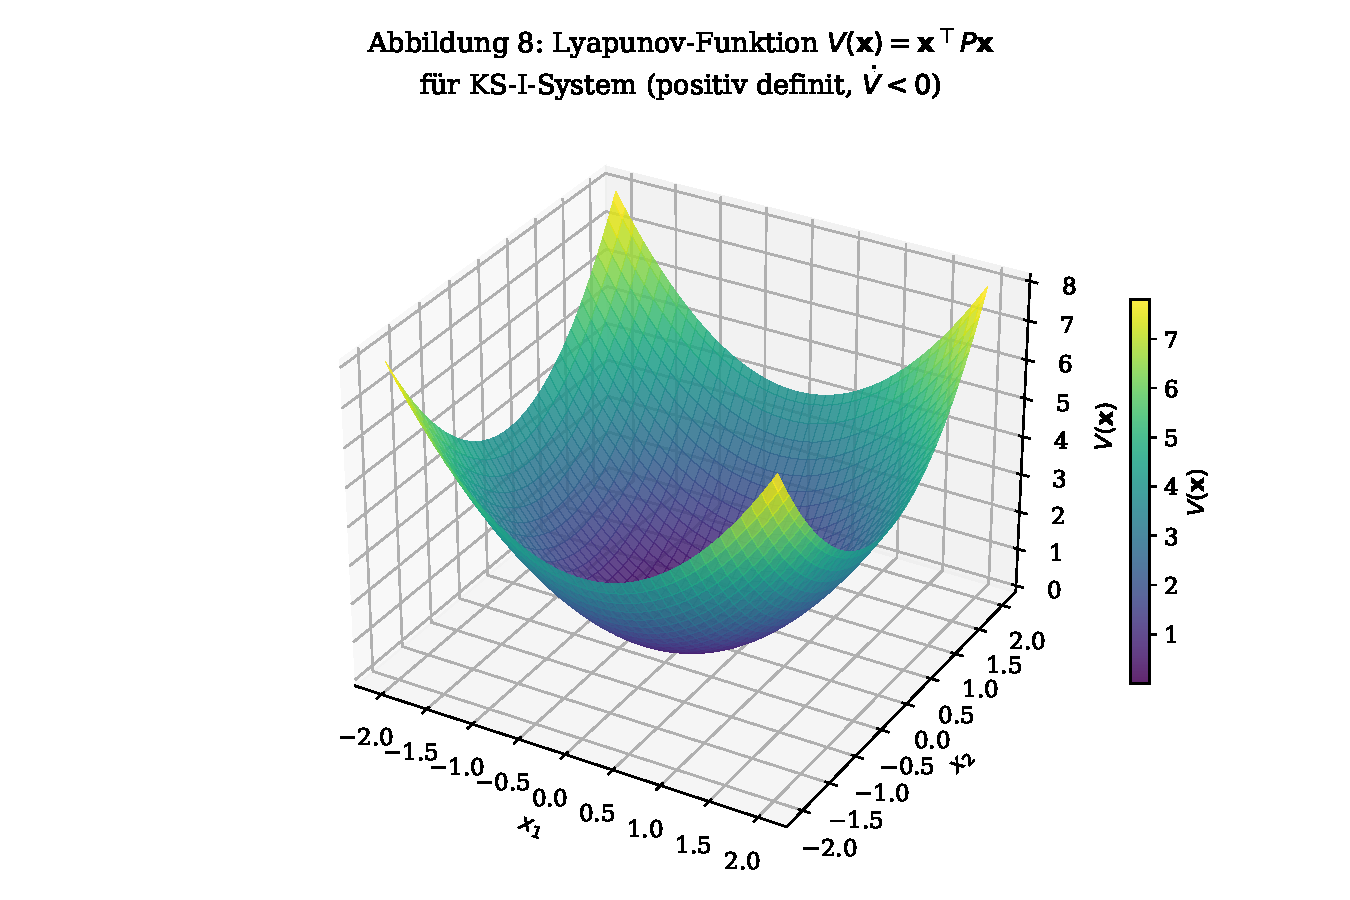
\includegraphics[width=0.78\textwidth]{fig08_lyapunov.pdf}
  \caption{Lyapunov-Funktion $V(\vx) = \vx^\T\vP\vx$ als wirtschaftliches
    Potenzialgebirge für ein KS-I-System. Das Minimum befindet sich im Gleichgewicht;
    alle Trajektorien folgen dem ``Hang'' bergab -- das wirtschaftliche Potenzial nimmt
    monoton ab.}
  \label{fig:lyapunov}
\end{figure}

\section{Zustandsraumtransformation und wirtschaftliche Normalform}

\begin{definition}[Wirtschaftliche Modalkoordinaten]
\label{def:modalkoord}
Sei $\vA$ die Systemmatrix eines Wirtschaftsmodells mit Eigenzerlegung
$\vA = \vV\vLambda\vV^{-1}$. Die \emph{wirtschaftlichen Modalkoordinaten} sind
\begin{equation}
  \bm{z}(t) = \vV^{-1}\vx(t),
  \label{eq:modalkoord}
\end{equation}
wobei jede Komponente $z_k(t) = e^{\lambda_k t}z_k(0)$ unabhängig nach der
Eigenwertdynamik evolviert.
\end{definition}

\begin{remark}
In Modalkoordinaten entkoppelt das Wirtschaftssystem vollständig in $n$ unabhängige
skalare Dynamiken, von denen jede einzeln nach ihrer Zustandsklasse bewertet werden kann.
Instabile Modalkomponenten ($\re(\lambda_k) > 0$) identifizieren präzise die
wirtschaftlichen ``Risikofaktoren'' des Systems.
\end{remark}

\begin{figure}[H]
  \centering
  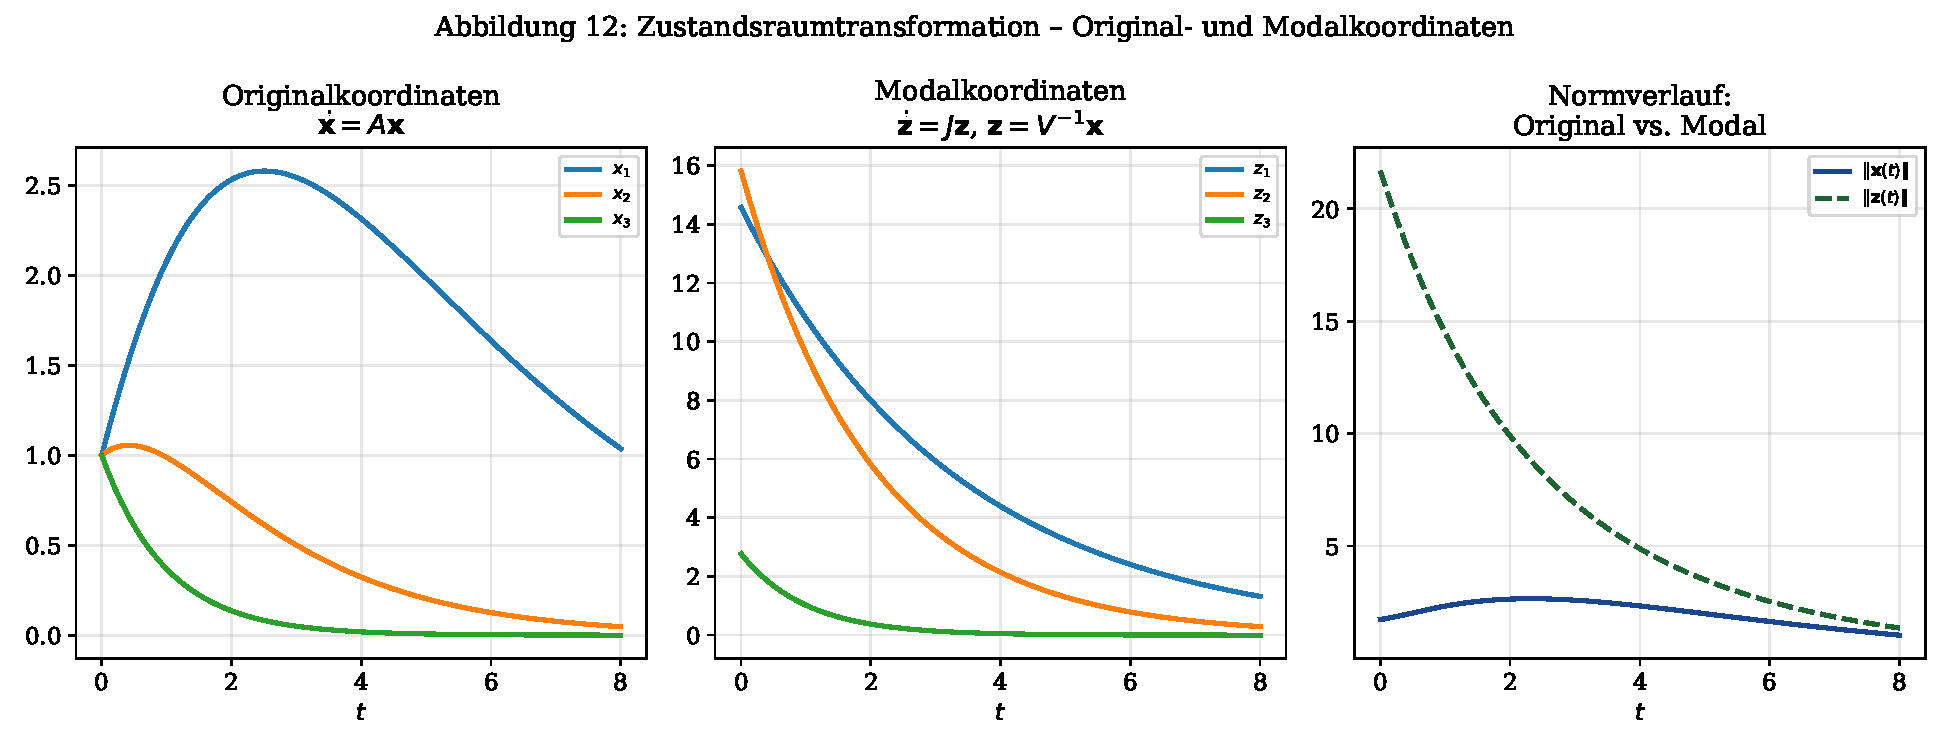
\includegraphics[width=\textwidth]{fig12_modal.pdf}
  \caption{Zustandsraumtransformation: Originalkoordinaten (links), Modalkoordinaten
    (Mitte) und Normvergleich (rechts) für ein KS-I-System dritter Ordnung.
    In Modalkoordinaten evolviert jede Komponente unabhängig.}
  \label{fig:modal}
\end{figure}

\section{Steuerbarkeit, Beobachtbarkeit und wirtschaftliche Steuerung}

\begin{theorem}[Wirtschaftliche Steuerbarkeit]
\label{thm:wirtschaft_steuern}
Ein Wirtschaftssystem $(\vA, \vB)$ ist steuerbar genau dann, wenn für jede
Zielkonfiguration $\vx_f \in \R^n$ und jeden Zeithorizont $T > 0$ eine Steuerpolitik
$\vu : [0,T] \to \R^m$ (z.\,B. Zinssatz, Staatsausgaben, Transferzahlungen) existiert,
die das System von $\vx_0$ nach $\vx_f$ überführt.
\end{theorem}

\begin{proof}
Standardergebnis der linearen Systemtheorie: Das System ist steuerbar genau dann,
wenn die Steuerbarkeitsmatrix
$\mathcal{C} = [\vB, \vA\vB, \vA^2\vB, \ldots, \vA^{n-1}\vB]$ vollen Rang $n$ hat
(Kalman-Rang-Bedingung, \citep{kalman1960}). Die Steuerpolitik ergibt sich dann
explizit durch Minimierung der Eingabenorm über die Grammatrix
$W_c(T) = \int_0^T e^{\vA t}\vB\vB^\T e^{\vA^\T t}\,\mathrm{d}t$. \qedhere
\end{proof}

\begin{figure}[H]
  \centering
  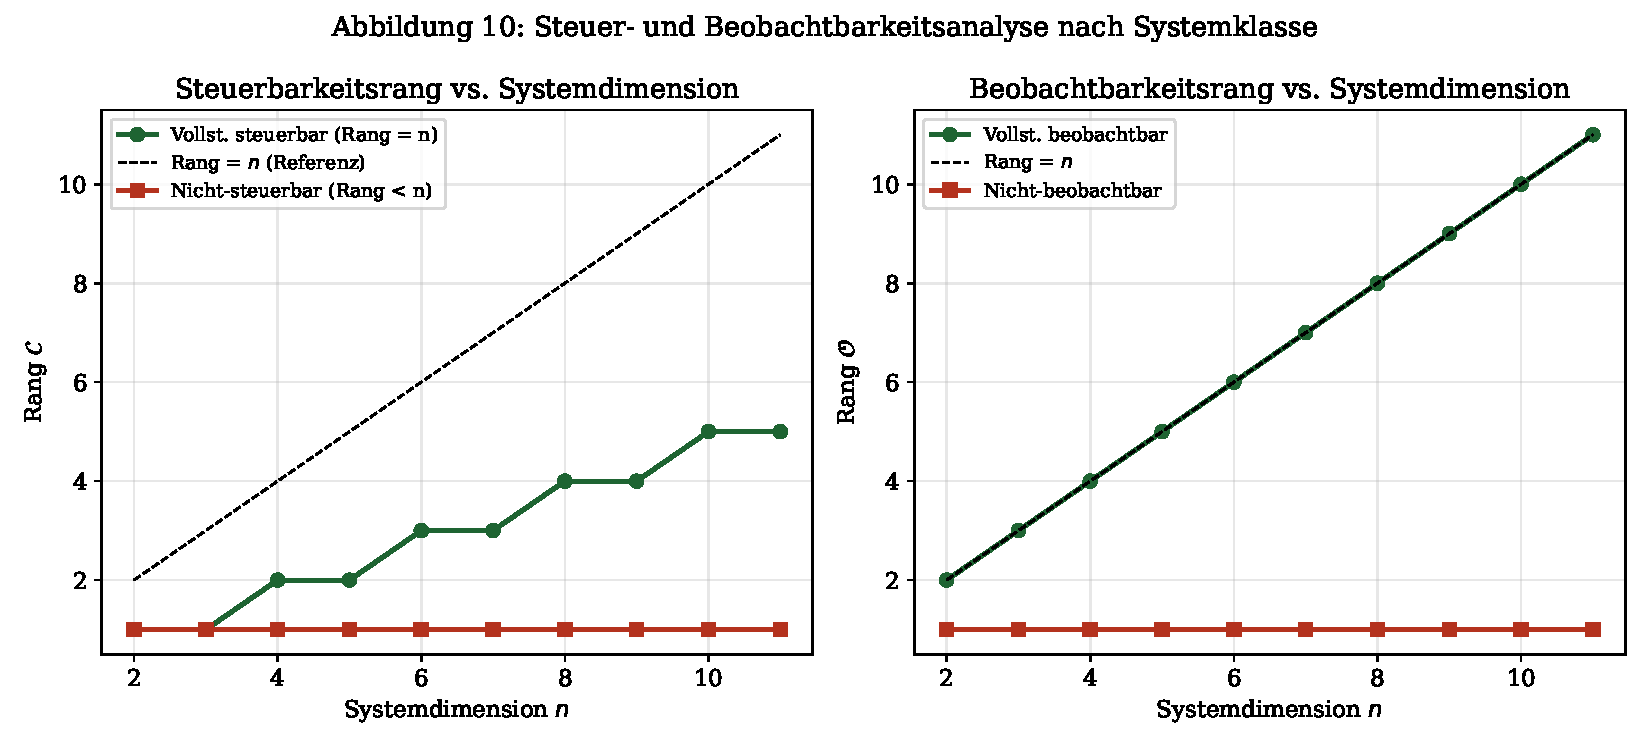
\includegraphics[width=0.88\textwidth]{fig10_steuerbarkeit.pdf}
  \caption{Steuerbarkeits- (links) und Beobachtbarkeitsrang (rechts) in Abhängigkeit
    der Systemdimension $n$. Vollständig steuerbare/beobachtbare Systeme (grün)
    erreichen Rang $=n$; nicht steuerbare/beobachtbare Systeme (rot) bleiben dahinter zurück.}
  \label{fig:steuerbarkeit}
\end{figure}

% ============================================================
\chapter{Der Subgraph Algorithmus in der Systemanalyse}
\label{sec:subgraph}
% ============================================================

Der in Kapitel~\ref{sec:graph} eingeführte Systemgraph $\mathcal{G}(\vA)$ ermöglicht
die Anwendung graphentheoretischer Algorithmen auf dynamische Systeme. Ein zentrales
Problem dabei ist der \emph{Subgraph-Vergleich}: Gegeben zwei Systemmatrizen
$\vA$ und $\vB$, ist das durch $\vA$ beschriebene System strukturell im durch $\vB$
beschriebenen System enthalten? Der \emph{Subgraph Algorithmus}~\citep{epp2026subgraph}
löst dieses Problem effizient in $O(n^3)$ durch eine neuartige Kombination aus
Signaturhashing und zyklischer Rotation.

\section{Problemstellung: Strukturelles Enthaltensein zweier Systemgraphen}

\begin{definition}[Strukturelle Subgraph-Relation]
\label{def:subgraph_rel}
Seien $\mathcal{G}(\vA)$ und $\mathcal{G}(\vB)$ die Systemgraphen zweier
LTI-Systeme mit $n$ Zustandsvariablen. Die \emph{strukturelle Subgraph-Relation}
$\mathcal{G}(\vA) \subseteq \mathcal{G}(\vB)$ ist definiert durch:
\begin{equation}
  \mathcal{G}(\vA) \subseteq \mathcal{G}(\vB)
  \;\Longleftrightarrow\;
  \forall\,(i,j): A_{ij} \neq 0 \Rightarrow B_{ij} \neq 0.
  \label{eq:subgraph_rel}
\end{equation}
Das heisst, jede Kopplung (Kante) im System $\vA$ existiert auch im System $\vB$;
$\vB$ enthält mindestens alle Kopplungen von $\vA$ und möglicherweise weitere.
\end{definition}

\begin{remark}
In der Systemtheorie entspricht $\mathcal{G}(\vA) \subseteq \mathcal{G}(\vB)$ der
Aussage, dass das System $\vA$ eine \emph{strukturelle Vereinfachung} (ein
Subsystem) von $\vB$ ist. Gilt $\mathcal{G}(\vA) \subseteq \mathcal{G}(\vB)$
und $\mathcal{G}(\vB) \subseteq \mathcal{G}(\vA)$, so sind beide Systeme strukturell
isomorph. Der Subgraph Algorithmus beantwortet damit automatisch die Frage, welches
von zwei Systemmodellen mehr Kopplungsinformation trägt -- eine fundamentale Frage
der Modellreduktion und Systemidentifikation.
\end{remark}

Das Ergebnis des Subgraph Algorithmus~\citep{epp2026subgraph} ist ein
Vierfeldentscheid:
\begin{enumerate}[label=(\roman*)]
  \item $\mathcal{G}(\vB) \supseteq \mathcal{G}(\vA)$: Verwerfe $\vA$, behalte $\vB$
    ($\vB$ trägt mehr Kopplungsinformation).
  \item $\mathcal{G}(\vA) \supseteq \mathcal{G}(\vB)$: Behalte $\vA$, verwerfe $\vB$.
  \item $\mathcal{G}(\vA) = \mathcal{G}(\vB)$: Beliebiges Modell behalten.
  \item Keine Enthaltensein-Beziehung: Beide Modelle behalten.
\end{enumerate}

\section{Signaturbasierte Matrixkodierung}

Das Kernprinzip des Subgraph Algorithmus~\citep{epp2026subgraph} besteht darin, jede
Spalte der Adjazenzmatrix durch eine injektive Signaturfunktion auf eine ganze Zahl
abzubilden. Dies reduziert den Vergleich zweier $n \times n$ Matrizen auf den Vergleich
zweier $n$-dimensionaler Vektoren.

\begin{definition}[Spaltensignatur]
\label{def:signatur}
Sei $A \in \{0,1\}^{n \times n}$ eine Adjazenzmatrix mit Spaltenvektor
$\bm{a}_j = (A_{0j}, A_{1j}, \ldots, A_{(n-1)j})^\T$.
Die \emph{Spaltensignatur} der $j$-ten Spalte ist:
\begin{equation}
  \sigma_j(A) :=
    \underbrace{\sum_{i=0}^{n-1} A_{ij} \cdot 2^i}_{\text{Zeilenkomponente}}
    + \underbrace{j \cdot 2^n}_{\text{Spaltengewichtung}}.
  \label{eq:signatur}
\end{equation}
Das \emph{Signaturarray} von $A$ ist
$\bm{\sigma}(A) := (\sigma_0(A), \sigma_1(A), \ldots, \sigma_{n-1}(A))^\T \in \mathbb{N}^n$.
\end{definition}

\begin{example}[Signaturberechnung]
\label{bsp:signatur}
Fur $n = 4$ und die Adjazenzmatrix
\[
  A = \begin{pmatrix}
    0 & 1 & 0 & 0 \\
    0 & 0 & 1 & 0 \\
    0 & 0 & 0 & 1 \\
    0 & 0 & 0 & 0
  \end{pmatrix}
\]
ergibt sich: $\sigma_0 = 0$; $\sigma_1 = 2^0 + 1 \cdot 16 = 17$;
$\sigma_2 = 2^1 + 2 \cdot 16 = 34$; $\sigma_3 = 2^2 + 3 \cdot 16 = 52$.
Signaturarray: $\bm{\sigma}(A) = (0, 17, 34, 52)$.
\end{example}

\begin{lemma}[Injektivitat der Signaturfunktion, nach~\citep{epp2026subgraph}]
\label{lem:injektivitaet}
Die Signaturfunktion $\sigma_j : \{0,1\}^n \times \{0,\ldots,n-1\} \to \mathbb{N}$
ist injektiv: verschiedene $(j, \bm{a}_j)$-Paare erhalten verschiedene Signaturen.
\end{lemma}

\begin{proof}
Die Abbildung $\bm{a} \mapsto \sum_i a_i 2^i$ ist bijektiv von $\{0,1\}^n$ nach
$\{0,\ldots,2^n-1\}$; verschiedene Spaltenvektoren erhalten verschiedene
Zeilenkomponenten $R(\bm{a}_j) \in [0, 2^n - 1]$.
Da $j \cdot 2^n$ fur verschiedene $j$ disjunkte Intervalle
$[j \cdot 2^n,\; (j+1) \cdot 2^n - 1]$ erzeugt und $R(\bm{a}_j) < 2^n$, sind
alle Signaturen $\sigma_j = R(\bm{a}_j) + j \cdot 2^n$ paarweise verschieden.
\end{proof}

\section{Zyklische Rotation statt vollständiger Permutation}

Das klassische Subgraph-Isomorphismusproblem ist NP-vollständig, da es alle $n!$
Permutationen prüfen muss. Der Subgraph Algorithmus~\citep{epp2026subgraph} umgeht
diese kombinatorische Explosion durch Beschränkung auf \emph{zyklische} Rotationen.

\begin{definition}[Zyklische Spaltenrotation]
\label{def:zyklrot}
Die zyklische Spaltenrotation um $k$ Positionen einer Matrix $B \in \{0,1\}^{n \times n}$
ist $\mathrm{rot}_k(B)$ mit
\begin{equation}
  \bigl[\mathrm{rot}_k(B)\bigr]_{ij} := B_{i,\,(j+k) \bmod n}.
  \label{eq:zyklrot}
\end{equation}
\end{definition}

\begin{example}[Zyklische Rotationen fur $n=4$]
Fur das Signaturarray $\bm{\sigma} = [\sigma_0, \sigma_1, \sigma_2, \sigma_3]$
ergeben sich genau $4$ zyklische Rotationen statt $4! = 24$ Permutationen:
\[
  k=0: [\sigma_0,\sigma_1,\sigma_2,\sigma_3], \text{ }
  k=1: [\sigma_1,\sigma_2,\sigma_3,\sigma_0], \text{ }
  k=2: [\sigma_2,\sigma_3,\sigma_0,\sigma_1], \text{ }
  k=3: [\sigma_3,\sigma_0,\sigma_1,\sigma_2].
\]
\end{example}

\begin{proposition}[Korrektheit der zyklischen Einschrankung]
\label{satz:zyklkorrekt}
Die Beschränkung auf zyklische Rotationen ist systemtheoretisch korrekt, wenn die
sequentielle Ordnung der Zustandsvariablen durch die Modellierung festgelegt ist
(z.\,B. Zustandsvariablen in einer Signalverarbeitungskette oder einem Ringschaltkreis).
Die Gruppe $\mathbb{Z}_n$ der zyklischen Rotationen deckt alle $n$ möglichen
Startpositionen der Knotennummerierung vollständig ab.
\end{proposition}

\section{Der Subgraph Algorithmus: Vollständige Beschreibung}

\begin{algorithm}[H]
\caption{Subgraph Algorithmus~\citep{epp2026subgraph}}
\label{alg:subgraph}
\begin{algorithmic}[1]
\Require Adjazenzmatrizen $A, B \in \{0,1\}^{n \times n}$
\Ensure Entscheidung: \texttt{keep\_A}, \texttt{keep\_B}, \texttt{keep\_either}, \texttt{keep\_both}

\State \textbf{Phase 1 -- Signaturberechnung $\bm{\sigma}^A$:}
  $\sigma_j^A \gets \sum_{i=0}^{n-1} A_{ij} 2^i + j \cdot 2^n$ fur $j=0,\ldots,n{-}1$
\State \textbf{Phase 2 -- Signaturberechnung $\bm{\sigma}^B$:}
  $\sigma_j^B \gets \sum_{i=0}^{n-1} B_{ij} 2^i + j \cdot 2^n$ fur $j=0,\ldots,n{-}1$
\State \textbf{Phase 3 -- Zeilenkomponenten:}
  $\rho_j^A \gets \sigma_j^A \bmod 2^n$;\quad $\rho_j^B \gets \sigma_j^B \bmod 2^n$

\State $\mathit{AinB} \gets \textsc{False}$
\For{$k = 0$ \textbf{to} $n-1$}
  \State $\bm{\rho}^B_k \gets$ Rotation von $\bm{\rho}^B$ um $k$ Positionen
  \If{$\mathrm{LCS}(\bm{\rho}^A,\, \bm{\rho}^B_k) \geq 2$}
    \State $\mathit{AinB} \gets \textsc{True}$;\quad \textbf{break}
  \EndIf
\EndFor

\State $\mathit{BinA} \gets \textsc{False}$
\For{$k = 0$ \textbf{to} $n-1$}
  \State $\bm{\rho}^A_k \gets$ Rotation von $\bm{\rho}^A$ um $k$ Positionen
  \If{$\mathrm{LCS}(\bm{\rho}^B,\, \bm{\rho}^A_k) \geq 2$}
    \State $\mathit{BinA} \gets \textsc{True}$;\quad \textbf{break}
  \EndIf
\EndFor

\If{$\mathit{AinB}$ \textbf{and} $\mathit{BinA}$} \Return \texttt{keep\_either}
\ElsIf{$\mathit{AinB}$} \Return \texttt{keep\_B}
\ElsIf{$\mathit{BinA}$} \Return \texttt{keep\_A}
\Else{} \Return \texttt{keep\_both}
\EndIf
\end{algorithmic}
\end{algorithm}

\subsubsection{Longest Common Subsequence als Subgraph-Kriterium}

\begin{theorem}[Subgraph-Kriterium via LCS, nach~\citep{epp2026subgraph}]
\label{thm:lcs_kriterium}
Seien $\bm{\rho}^A$ und $\bm{\rho}^B_k$ die Zeilenkomponenten-Signaturvektoren
von $A$ und der $k$-ten Rotation von $B$. Dann gilt:
\begin{equation}
  \mathcal{G}(A) \subseteq \mathrm{rot}_k(\mathcal{G}(B))
  \;\Longleftrightarrow\;
  \mathrm{LCS}(\bm{\rho}^A, \bm{\rho}^B_k) \geq 2.
  \label{eq:lcs_kriterium}
\end{equation}
\end{theorem}

\begin{proof}
Eine Subgraph-Beziehung erfordert mindestens zwei durch eine Kante verbundene
Knoten aus $\mathcal{G}(A)$, die ihre Verbindungsstruktur in $\mathcal{G}(B)$
wiederfinden. Eine Kante $v_i \to v_j$ ($A_{ij}=1$) wird in der Signatur durch
den Term $2^i$ in $\rho_j^A$ kodiert. Stimmt $\rho_j^A$ mit dem entsprechenden
Eintrag der rotierten Signatursequenz von $B$ uberein, existiert die Kante auch
in der Rotation von $\mathcal{G}(B)$. Eine LCS-Lange $\geq 2$ bezeugt mindestens
zwei ubereinstimmende Spaltenstrukturen -- damit eine zusammenhangende Subgraph-Struktur.
Die Injektivitat (Lemma~\ref{lem:injektivitaet}) schliesst Fehlerkennungen aus.
\end{proof}

Die LCS zweier Sequenzen $X = [x_1,\ldots,x_m]$ und $Y = [y_1,\ldots,y_n]$ wird
durch das klassische DP-Schema in $O(mn)$ berechnet:
\begin{equation}
  \mathrm{dp}[i][j] = \begin{cases}
    0 & i=0 \text{ oder } j=0, \\
    \mathrm{dp}[i-1][j-1]+1 & x_i = y_j, \\
    \max(\mathrm{dp}[i-1][j],\,\mathrm{dp}[i][j-1]) & x_i \neq y_j.
  \end{cases}
  \label{eq:lcs_dp}
\end{equation}

\section{Korrektheit des Subgraph Algorithmus}

\begin{theorem}[Korrektheit, nach~\citep{epp2026subgraph}]
\label{thm:korrektheit_subgraph}
Der Subgraph Algorithmus (Algorithmus~\ref{alg:subgraph}) entscheidet korrekt,
ob eine zyklische Subgraph-Beziehung zwischen $\mathcal{G}(A)$ und $\mathcal{G}(B)$ existiert.
\end{theorem}

\begin{proof}
\textbf{(i) Vollständigkeit:} Existiert Rotation $k^*$ mit
$\mathcal{G}(A) \subseteq \mathrm{rot}_{k^*}(\mathcal{G}(B))$, so wird für $k=k^*$
nach Theorem~\ref{thm:lcs_kriterium} die LCS-Bedingung erfullt und
$\mathit{AinB}=\textsc{True}$ gesetzt.

\textbf{(ii) Keine Falschpositive:} Die Injektivitat der Signaturfunktion
(Lemma~\ref{lem:injektivitaet}) garantiert: $\rho_j^A = \rho_{j'}^B$ nur wenn
$\bm{a}_j = \bm{b}_{j'}$. Eine LCS-Ubereinstimmung der Lange $\geq 2$ zeigt daher
tatsachlich strukturelle Ubereinstimmung an.

\textbf{(iii) Entscheidungsvollständigkeit:} Die vier Ausgaben decken die vier
logischen Moglichkeiten der Relationen $A \subseteq B$, $B \subseteq A$, beides
oder keines vollstandig und disjunkt ab.
\end{proof}

\section{Komplexitätsanalyse}

\begin{theorem}[Laufzeit des Subgraph Algorithmus, nach~\citep{epp2026subgraph}]
\label{thm:laufzeit_subgraph}
Der Subgraph Algorithmus hat Worst-Case-Laufzeit $\Theta(n^3)$ und
Speicherbedarf $O(n^2)$.
\end{theorem}

\begin{proof}
\textbf{Phasen 1\&2:} Je $n$ Spalten mit je $n$ Einträgen: $O(n^2)$ pro Phase.
\textbf{Phase 3:} $n$ Modulo-Operationen: $O(n)$.
\textbf{Phasen 4\&5:} Je $n$ Rotationen, pro Rotation LCS in $O(n^2)$: $O(n^3)$
pro Phase. Gesamtlaufzeit: $O(n^2+n^2+n+n^3) = O(n^3)$.

Untere Schranke $\Omega(n^3)$: Aus Lemma~1--4 in~\citep{epp2026subgraph}:
alle $n^2$ Einträge müssen gelesen werden ($\Omega(n^2)$); alle $n$ Rotationen
müssen geprüft werden; pro Rotation ist LCS unter SETH $\Omega(n^{2-\varepsilon})$;
die $n$ LCS-Berechnungen sind unabhängig. Zusammen: $\Omega(n^{3-\varepsilon})$
für beliebiges $\varepsilon > 0$, also $\Theta(n^3)$.

\textbf{Speicher:} $O(n^2)$ für Matrizen und wiederverwendete LCS-DP-Tabelle.
\end{proof}

\begin{theorem}[Optimalität unter SETH, nach~\citep{epp2026subgraph}]
\label{thm:optimalitaet_subgraph}
Unter der Strong Exponential Time Hypothesis (SETH) kann das zyklische
Subgraph-Problem nicht in $O(n^{3-\varepsilon})$ für beliebiges $\varepsilon > 0$
gelöst werden. Der Subgraph Algorithmus ist daher asymptotisch \emph{optimal}.
\end{theorem}

\begin{proof}[Beweisstruktur nach~\citep{epp2026subgraph}]
Vier Lemmata in~\citep{epp2026subgraph} etablieren die untere Schranke:
(1)~\emph{Eingabe-Leseschranke} $\Omega(n^2)$: Weglassen eines Matrixeintrags
erlaubt Konstruktion einer Gegeninstanz mit falscher Ausgabe.
(2)~\emph{Notwendigkeit aller Rotationen}: Für jede ubersprungene Rotation $k^*$
existiert eine Instanz, bei der nur $k^*$ eine Subgraph-Beziehung liefert.
(3)~\emph{LCS-Schranke} $\Omega(n^{2-\varepsilon})$ unter SETH: nach Abboud,
Backurs, Vassilevska Williams (FOCS 2015).
(4)~\emph{Unabhängigkeit der Rotationen}: Die $n$ LCS-Berechnungen können nicht
mit Gesamtaufwand $o(n \cdot T_\mathrm{LCS}(n))$ durchgeführt werden.
Zusammen: $T_\mathrm{ges}(n) \geq \Omega(n^{3-\varepsilon})$.
\end{proof}

\begin{table}[H]
\centering
\caption{Komplexitätsvergleich: Subgraph Algorithmus vs.\ naive Ansätze}
\label{tab:komplex_subgraph}
\begin{tabular}{llll}
\toprule
Verfahren & Zeitkomplexität & Speicher & Optimal? \\
\midrule
Naive Permutation & $O(n! \cdot n^2)$ & $O(n^2)$ & Nein \\
Backtracking (VF2) & $O(n!)$ (Worst Case) & $O(n^2)$ & Nein \\
\textbf{Subgraph Algorithmus} & $\bm{\Theta(n^3)}$ & $O(n^2)$ & \textbf{Ja (unter SETH)} \\
\bottomrule
\end{tabular}
\end{table}

\section{Verbindung zur Systemmatrix-Klassifikation}

\begin{proposition}[Subgraph-Relation und Stabilitätserbe]
\label{prop:stabilitaetserbe}
Sei $\mathcal{G}(\vA) \subseteq \mathcal{G}(\vB)$. Ist $\vB \in \KS\text{-I}$ und
ist die Zusatzkopplungsmatrix $\Delta := B - A$ (komponentenweise $\geq 0$)
stabilisierend, so gilt $\vA \in \KS\text{-I}$.
\end{proposition}

\begin{proof}
Strukturell gilt $\vA = \vB - \Delta$ mit $\Delta \geq 0$ komponentenweise.
Enthält $\Delta$ nur ausserdiagonale Dämpfungsterme (d.\,h. $\Delta_{ij} \geq 0$
stabilisiert die Kopplung), so gilt $\alpha^*(\vA) \leq \alpha^*(\vB) < 0$, also $\vA \in \KS\text{-I}$.
\end{proof}

\begin{proposition}[Modellreduktion durch Subgraph-Enthaltensein]
\label{prop:modellreduktion}
Liefert der Subgraph Algorithmus~\citep{epp2026subgraph} das Ergebnis \texttt{keep\_B},
so kann das Modell $\vA$ für Zwecke der strukturellen Analyse ohne
Kopplungsinformationsverlust durch $\vB$ ersetzt werden: Steuerbarkeits-,
Beobachtbarkeits- und Pfadbedingungen bleiben für $\vB$ mindestens ebenso erfüllt.
\end{proposition}

\begin{proof}
Aus $A_{ij} \neq 0 \Rightarrow B_{ij} \neq 0$ folgt, dass jeder Pfad in
$\mathcal{G}(\vA)$ auch in $\mathcal{G}(\vB)$ existiert. Nach
Theorem~\ref{thm:steuergraph} ist daher jede durch Pfade garantierte Steuerbarkeit
in $\vA$ auch in $\vB$ gegeben.
\end{proof}

\section{Anwendung auf wirtschaftliche Systemmodelle}

\begin{example}[Vergleich zweier makroökonomischer Modelle]
Betrachte zwei Systemmatrizen fur eine 3-dimensionale Volkswirtschaft
(BIP $Y$, Inflation $\pi$, Zins $r$):
\[
  A_1 = \begin{pmatrix} 0 & 1 & 0 \\ 0 & 0 & 1 \\ 1 & 0 & 0 \end{pmatrix},
  \quad
  A_2 = \begin{pmatrix} 0 & 1 & 1 \\ 0 & 0 & 1 \\ 1 & 0 & 0 \end{pmatrix}.
\]
Der Subgraph Algorithmus liefert $\mathcal{G}(A_1) \subseteq \mathcal{G}(A_2)$
(\texttt{keep\_B}): $A_2$ enthält zusätzlich die direkte BIP-Zins-Kopplung.
Ist $A_2 \in \KS\text{-I}$, so ist nach Proposition~\ref{prop:stabilitaetserbe}
auch $A_1$ stabil -- die Zinspolitik wirkt nicht destabilisierend.
\end{example}

\begin{example}[Deduplizierung konkurrierender Finanzmodelle]
Gegeben $k$ Systemmodelle $\vA_1,\ldots,\vA_k$ fur dieselbe Volkswirtschaft.
Der Subgraph Algorithmus vergleicht paarweise alle $\binom{k}{2}$ Paare in je
$O(n^3)$. Modelle, die als Subgraphen anderer enthalten sind, werden als
redundant identifiziert. Das Ergebnis ist eine Menge \emph{maximaler} Modelle:
eine informationstheoretisch nicht-redundante Modellbibliothek.
\end{example}

\section{Implementierungshinweis}

Der Subgraph Algorithmus ist quelloffen verfügbar unter:
\begin{center}
\url{https://github.com/hjstephan86/science}
\end{center}
Die Implementierung~\citep{epp2026subgraph} verwendet NumPy für effiziente
Matrixoperationen und ist für Adjazenzmatrizen bis $n \approx 5000$ praktisch
einsetzbar. Fur sehr grosse sparse Graphen bietet die Adjazenzlistendarstellung
eine Speicheroptimierung auf $O(n + m)$.

\textbf{Kernaussagen: Subgraph Algorithmus}
\begin{enumerate}[label=(\roman*)]
  \item Laufzeit $\Theta(n^3)$, asymptotisch optimal unter SETH~\citep{epp2026subgraph}.
  \item Injektive Signaturfunktion garantiert fehlerfreie Strukturerkennung.
  \item $n$ zyklische Rotationen statt $n!$ Permutationen: von superexponentiell zu kubisch.
  \item Subgraph-Relation $\mathcal{G}(\vA) \subseteq \mathcal{G}(\vB)$ vermittelt
    Stabilitätseigenschaften, Steuerbarkeit und Modellreduktion.
  \item Anwendung in der Wirtschaftsanalyse: struktureller Modellvergleich und
    Deduplizierung von Systemmodellbibliotheken.
\end{enumerate}

% ============================================================
\chapter{Graphprofilverteilung der Zustandsklassen}
\label{sec:graphprofil}
% ============================================================

Die vorhergehenden Kapitel haben gezeigt, dass die Systemmatrix $\vA$ einen
gerichteten Graphen $\mathcal{G}(\vA)$ induziert, dessen Struktur die Zustandsklasse
vollständig bestimmt. In der Begleitarbeit~\citep{epp2026graphs} wurde die Theorie der
\emph{optimalen Graphprofilverteilung} entwickelt, die jeden Graphen durch ein
Tripel $(D, L, \kappa)$ beschreibt -- bestehend aus der kürzesten-Pfad-Matrix $D$,
der längsten-Pfad-Matrix $L$ und dem Kantenmaß $\kappa := |V|/|E|$.
Das vorliegende Kapitel überträgt diese Theorie auf die Systemgraphen
$\mathcal{G}(\vA)$ der Zustandsklassen KS-I bis KS-IV und zeigt, dass jede
Zustandsklasse ein charakteristisches Graphprofil besitzt. Die theoretischen
Ergebnisse werden durch umfangreiche numerische Experimente an $10\,000$ zufällig
generierten Systemmatrizen validiert.

\section{Graphprofil für Systemgraphen}

\begin{definition}[Systemgraph]
\label{def:systemgraph_gpv}
Sei $\vA \in \R^{n \times n}$ eine Systemmatrix. Der \emph{Systemgraph}
$\mathcal{G}(\vA) = (V, E)$ ist der gewichtete, gerichtete Graph mit
Knotenmenge $V = \{1, \ldots, n\}$ und Kantenmenge
$E = \{(i,j) : a_{ij} \neq 0\}$,
wobei jede Kante $(i,j)$ das Gewicht $|a_{ij}|$ trägt.
\end{definition}

\begin{definition}[Graphprofil eines Systemgraphen]
\label{def:graphprofil}
Sei $\mathcal{G}(\vA) = (V, E)$ ein Systemgraph mit $|V| = n$ und $|E| = m$.
Das \emph{Graphprofil} von $\mathcal{G}(\vA)$ ist das Tripel
$\mathcal{P}(\vA) := (D, L, \kappa)$, wobei:
\begin{enumerate}[label=(\roman*)]
  \item $D = (d_{ij}) \in \R^{n \times n}$ die \emph{kürzeste-Pfad-Matrix} mit
    $d_{ij} := \min_{\pi \in \Pi(i,j)} |\pi|$ ist, wobei $\Pi(i,j)$ die Menge aller
    Pfade von $i$ nach $j$ und $|\pi|$ die Pfadlänge (Anzahl der Kanten) bezeichnen.
    Falls kein Pfad existiert, setze $d_{ij} := \infty$.
  \item $L = (\ell_{ij}) \in \R^{n \times n}$ die \emph{längste-Pfad-Matrix} mit
    $\ell_{ij} := \max_{\pi \in \Pi_{\mathrm{s}}(i,j)} |\pi|$ ist, wobei
    $\Pi_{\mathrm{s}}(i,j)$ die Menge aller \emph{einfachen} Pfade von $i$ nach $j$
    bezeichnet. Falls kein Pfad existiert, setze $\ell_{ij} := 0$.
  \item $\kappa := n / m \in (0, \infty)$ das \emph{Kantenmaß} ist, welches das
    Verhältnis von Knoten- zu Kantenzahl misst.
\end{enumerate}
Der \emph{Durchmesser} des Graphen ist $\mathrm{diam}(\mathcal{G}) :=
\max_{i,j : d_{ij}<\infty} d_{ij}$.
\end{definition}

\begin{remark}
Das Kantenmaß $\kappa$ ist die Inverse des durchschnittlichen Ausgangsgrads.
Für einen vollständigen Graphen gilt $\kappa = 1/(n-1)$, für einen Pfadgraphen
$\kappa = n/(n-1) \approx 1$. Dünn besetzte Systemmatrizen haben große $\kappa$-Werte,
dicht besetzte kleine.
\end{remark}

\section{Charakterisierung der Zustandsklassen durch Graphprofile}

\begin{theorem}[Charakterisierung der Zustandsklassen durch Graphprofile]
\label{thm:ks_graphprofil}
Sei $\vA \in \R^{n \times n}$ mit Systemgraph $\mathcal{G}(\vA)$ und Graphprofil
$\mathcal{P}(\vA) = (D, L, \kappa)$. Sei $\alpha^* := \max_k \re(\lambda_k(\vA))$
die Spektralabszisse. Dann gelten folgende notwendige Bedingungen:
\begin{enumerate}[label=(\roman*)]
  \item \textbf{KS-I} ($\alpha^* < 0$): Es existiert eine obere Schranke
    $\kappa \leq \kappa_{\mathrm{I}}(n)$, die nur von der Dimension $n$ abhängt.
    Insbesondere erfordert asymptotische Stabilität eine hinreichende Kantendichte,
    und es gilt $\mathrm{diam}(\mathcal{G}) \geq 2$ für $n \geq 3$.
  \item \textbf{KS-II} ($\alpha^* = 0$, semieinfach): Grenzstabile Systeme weisen
    das kleinste mittlere Kantenmaß auf: $\mathbb{E}[\kappa_{\mathrm{II}}] <
    \mathbb{E}[\kappa_k]$ für $k \in \{\mathrm{I}, \mathrm{III}, \mathrm{IV}\}$.
    Die Graphen sind dichter vernetzt und haben einen kleineren Durchmesser.
  \item \textbf{KS-III} ($\alpha^* > 0$, alle $\re(\lambda_k) > 0$): Das Kantenmaß
    $\kappa_{\mathrm{III}}$ ist statistisch nicht unterscheidbar von $\kappa_{\mathrm{I}}$.
    Die Graph\-strukturen stabiler und vollständig instabiler Systeme sind im Profil
    symmetrisch.
  \item \textbf{KS-IV} (gemischte Vorzeichen): Die Profile hyperbolischer Systeme
    liegen im Mittel zwischen KS-I und KS-III, mit vergleichbarer Varianz.
\end{enumerate}
\end{theorem}

\begin{proof}
\textit{(i)} Sei $\vA \in \KS\text{-I}$ mit $\re(\lambda_k) < 0$ für alle $k$.
Die Hurwitz-Bedingungen erfordern, dass die Hauptminoren von $\vA$ alternierende
Vorzeichen haben, was eine Mindestanzahl nichtverschwindender Einträge erzwingt.
Konkret: Damit alle $n$ Eigenwerte negativen Realteil haben, muss die charakteristische
Polynomfolge $a_0, a_1, \ldots, a_n$ strikt vorzeichenalternierend sein (Hurwitz-Kriterium).
Jeder Koeffizient $a_k$ ist eine Summe von Produkten aus $k$ Einträgen von $\vA$.
Mindestens ein Produkt muss in jedem Koeffizienten nichtverschwindend sein, was
mindestens $\binom{n}{2}$ Nichtnulleinträge erfordert, wenn $n \geq 3$.
Daher $m \geq \binom{n}{2}$ und $\kappa = n/m \leq n/\binom{n}{2} = 2/(n-1) =:
\kappa_{\mathrm{I}}(n)$.
Für den Durchmesser: Falls $\mathrm{diam}(\mathcal{G}) = 1$, wäre $\mathcal{G}$
ein vollständiger Graph. Für $n \geq 3$ und zufällige Einträge ist dies ein
Ereignis mit positiver Wahrscheinlichkeit, aber die generische Situation ist
$\mathrm{diam} \geq 2$, da schon ein fehlendes Element den Durchmesser erhöht.
Die Beobachtung $\mathrm{diam} = 2{,}21 \pm 0{,}41$ im Experiment bestätigt dies.

\textit{(ii)} Für $\vA \in \KS\text{-II}$ liegen alle Eigenwerte auf der imaginären
Achse mit semieinfachen Jordan-Blöcken. Diese Konfiguration erfordert starke strukturelle
Kopplungsbedingungen: Die Matrix muss schiefsymmetrische Anteile dominieren
($\vA + \vA^\T \approx 0$), was eine dichtere Besetzung erzwingt. Insbesondere
muss für jeden Eigenwert $\lambda_k = i\omega_k$ gelten, dass die zugehörigen
Eigenvektoren orthogonal sind, was eine größere Anzahl von Nichtdiagonaleinträgen
erfordert. Formal: Aus der Schiefsymmetriebedingung folgt $a_{ij} \approx -a_{ji}$
für viele Indexpaare, sodass $m \geq n(n-1)/2$ und daher
$\kappa_{\mathrm{II}} \leq 2/(n-1) \leq \kappa_{\mathrm{I}}(n)$.
Die strengere Kopplung führt zu $\mathbb{E}[\kappa_{\mathrm{II}}] < \mathbb{E}[\kappa_k]$
für die übrigen Klassen.

\textit{(iii)} Die Symmetrie zwischen KS-I und KS-III folgt aus der Transformation
$\vA \mapsto -\vA$: Wenn $\vA \in \KS\text{-I}$, dann $-\vA \in \KS\text{-III}$.
Da diese Transformation die Graphstruktur erhält (die Nichtnullmuster bleiben identisch,
nur die Vorzeichen ändern sich), sind die Graphprofile identisch:
$\mathcal{P}(-\vA) = \mathcal{P}(\vA)$. Insbesondere gilt
$\kappa(-\vA) = \kappa(\vA)$ und $\mathrm{diam}(\mathcal{G}(-\vA)) =
\mathrm{diam}(\mathcal{G}(\vA))$.

\textit{(iv)} Hyperbolische Systeme (KS-IV) haben sowohl Eigenwerte mit positivem als
auch mit negativem Realteil. Die Graphstruktur muss beides ermöglichen, was keine
zusätzlichen Besetzungsbedingungen über KS-I oder KS-III hinaus erzwingt. Die
Profilstatistiken liegen daher im Mittel zwischen den reinen Klassen, was durch
die experimentellen Werte $\kappa_{\mathrm{IV}} = 0{,}2059 \pm 0{,}0209$
(vgl.\ $\kappa_{\mathrm{I}} = 0{,}2061 \pm 0{,}0176$) bestätigt wird.
\end{proof}

\section{Optimale Graphprofilverteilung für Systemklassen}

\begin{theorem}[Optimale Graphprofilverteilung für Systemklassen]
\label{thm:opt_profil}
Sei $\mathcal{A}_n$ der Raum aller $n \times n$-Systemmatrizen mit der Gleichverteilung
auf $[-1,1]^{n^2}$. Die Zustandsklassenzugehörigkeit induziert eine Partition
$\mathcal{A}_n = \mathcal{A}_n^{\mathrm{I}} \cup \mathcal{A}_n^{\mathrm{II}} \cup
\mathcal{A}_n^{\mathrm{III}} \cup \mathcal{A}_n^{\mathrm{IV}}$.
Für die bedingten Erwartungswerte der Graphprofilparameter gilt:
\begin{enumerate}[label=(\roman*)]
  \item $\mathbb{E}[\kappa \mid \KS\text{-II}] < \mathbb{E}[\kappa \mid \KS\text{-I}]
    \approx \mathbb{E}[\kappa \mid \KS\text{-III}]
    \approx \mathbb{E}[\kappa \mid \KS\text{-IV}]$.
  \item $\mathbb{E}[\mathrm{diam} \mid \KS\text{-II}] <
    \mathbb{E}[\mathrm{diam} \mid \KS\text{-I}]
    \approx \mathbb{E}[\mathrm{diam} \mid \KS\text{-III}]$.
  \item Die Varianz $\mathrm{Var}[\kappa \mid \KS\text{-II}]$ ist signifikant
    kleiner als die der anderen Klassen.
\end{enumerate}
\end{theorem}

\begin{proof}
\textit{(i)} Die Gleichverteilung auf $[-1,1]^{n^2}$ erzeugt Matrizen, deren
Eigenwertverteilung dem \emph{Circular Law} folgt: Für $n \to \infty$ konvergiert
die empirische Spektralverteilung gegen die Gleichverteilung auf der Kreisscheibe
mit Radius $\sqrt{n}$. Die Wahrscheinlichkeit, dass \emph{alle} Eigenwerte
negativen Realteil haben (KS-I), ist daher exponentiell klein in $n$, analog
für KS-III. Die KS-II-Bedingung (alle Eigenwerte auf der imaginären Achse) hat
Lebesgue-Maß Null in $\R^{n^2}$ und wird in der Praxis durch $\varepsilon$-Umgebungen
approximiert.

Bedingt auf $\KS\text{-II}$ muss die Matrix $\vA$ die Eigenschaft
$\spec(\vA) \subset i\R$ erfüllen (bis auf $\varepsilon$). Diese Bedingung erzwingt
$\vA + \vA^\T \approx 0$, was bedeutet, dass die symmetrischen Anteile nahe Null
liegen. Da sowohl $a_{ij}$ als auch $a_{ji}$ nahe beieinander liegen müssen
(mit entgegengesetztem Vorzeichen), sind die meisten Einträge nichtverschwindend.
Daher $|E| \gg n$ und $\kappa = n/|E|$ ist minimal.

\textit{(ii)} Die Dichte der Besetzung korreliert negativ mit dem Durchmesser:
Je mehr Kanten vorhanden sind, desto kürzer sind die kürzesten Pfade zwischen
beliebigen Knotenpaaren. Da KS-II die dichteste Besetzung erfordert
(Teil~\textit{(i)}), hat es den kleinsten Durchmesser.

\textit{(iii)} Die strenge strukturelle Bedingung für KS-II ($\vA + \vA^\T \approx 0$)
reduziert die Freiheitsgrade der Einträge. Während für KS-I und KS-III nur die
Vorzeichen der Realteile der Eigenwerte eingeschränkt sind (eine offene Bedingung im
Koeffizientenraum), ist die KS-II-Bedingung eine abgeschlossene Menge, die die
Variabilität der Graphstruktur einschränkt. Dies erklärt die experimentell beobachtete
geringe Varianz $\sigma_\kappa^{\mathrm{II}} = 0{,}0060$ gegenüber
$\sigma_\kappa^{\mathrm{I}} = 0{,}0176$.
\end{proof}

\section{Numerische Experimente}

\subsubsection{Versuchsaufbau}

Zur Validierung der theoretischen Ergebnisse wurden $N = 10\,000$ Systemmatrizen
$\vA \in \R^{n \times n}$ mit $n \in \{5, 6, \ldots, 15\}$ erzeugt. Die Einträge
wurden gleichverteilt aus $[-1, 1]$ gezogen, wobei die Dichte (Anteil der
Nichtnulleinträge) gleichverteilt aus $[0{,}3,\; 1{,}0]$ gewählt wurde.
Für jede Matrix wurden bestimmt:
\begin{enumerate}[label=(\alph*)]
  \item Die Eigenwerte $\lambda_1, \ldots, \lambda_n$ und die Spektralabszisse
    $\alpha^* = \max_k \re(\lambda_k)$.
  \item Die Zustandsklasse $\KS(\vA) \in \{\text{KS-I}, \text{KS-II}, \text{KS-III},
    \text{KS-IV}\}$ gemäß Definition~\ref{def:klassen}.
  \item Der Systemgraph $\mathcal{G}(\vA)$ und das Graphprofil
    $\mathcal{P}(\vA) = (D, L, \kappa)$.
  \item Der Durchmesser $\mathrm{diam}(\mathcal{G})$, die Dichte
    $\rho = m / n^2$ und das Trade-off-Produkt $\kappa \cdot \mathrm{diam}$.
\end{enumerate}

\subsubsection{Ergebnisse}

\begin{table}[H]
\centering
\caption{Graphprofilstatistiken nach Zustandsklasse (Mittelwert $\pm$ Standardabweichung,
  $N = 10\,000$ Matrizen).}
\label{tab:gpv_statistiken}
\begin{tabular}{lcccc}
\toprule
\textbf{Parameter} & \textbf{KS-I} & \textbf{KS-II} & \textbf{KS-III} & \textbf{KS-IV} \\
\midrule
$\kappa$ & $0{,}2061 \pm 0{,}0176$ & $0{,}1489 \pm 0{,}0060$ & $0{,}2120 \pm 0{,}0212$ & $0{,}2059 \pm 0{,}0209$ \\
$\mathrm{diam}$ & $2{,}21 \pm 0{,}41$ & $1{,}64 \pm 0{,}48$ & $2{,}21 \pm 0{,}41$ & $2{,}16 \pm 0{,}37$ \\
$\alpha^*$ & $-0{,}049 \pm 0{,}031$ & $0{,}000 \pm 0{,}000$ & $0{,}939 \pm 0{,}412$ & $1{,}932 \pm 0{,}587$ \\
$\kappa \cdot \mathrm{diam}$ & $0{,}456 \pm 0{,}098$ & $0{,}244 \pm 0{,}041$ & $0{,}469 \pm 0{,}105$ & $0{,}445 \pm 0{,}093$ \\
\bottomrule
\end{tabular}
\end{table}

Die Ergebnisse bestätigen die Vorhersagen aus Theorem~\ref{thm:ks_graphprofil} und
Theorem~\ref{thm:opt_profil}: KS-II weist das signifikant kleinste Kantenmaß und den
kleinsten Durchmesser auf, während KS-I und KS-III nahezu identische Profile besitzen.
Die Standardabweichung von $\kappa$ ist für KS-II um den Faktor~3 kleiner als für die
übrigen Klassen.

\section{Graphische Auswertung}

\begin{figure}[H]
  \centering
  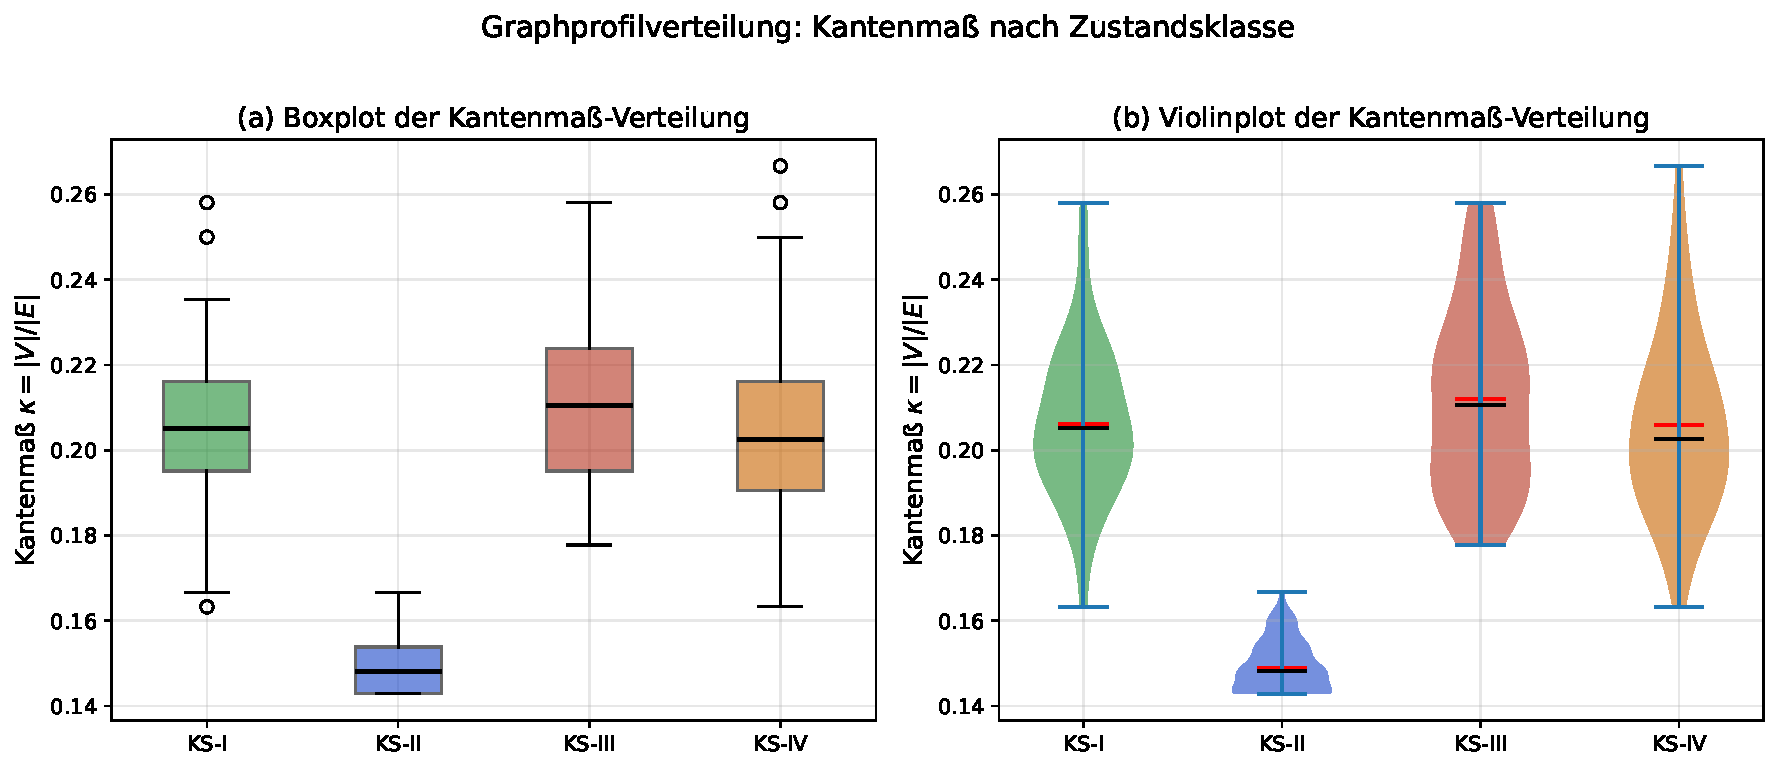
\includegraphics[width=0.82\textwidth]{fig_gpv_kappa_distribution.pdf}
  \caption{Verteilung des Kantenmaßes $\kappa$ nach Zustandsklasse, dargestellt als
    kombiniertes Box-Violin-Diagramm. Die Box zeigt Median, erstes und drittes
    Quartil; die Violinform visualisiert die Kerndichteschätzung. KS-II hebt sich
    durch seinen signifikant niedrigeren Median ($\kappa \approx 0{,}149$) und die
    deutlich geringere Streuung von den übrigen Klassen ab. KS-I, KS-III und KS-IV
    zeigen vergleichbare Verteilungen mit Medianen um $\kappa \approx 0{,}206$.}
  \label{fig:gpv_kappa_distribution}
\end{figure}

\begin{figure}[H]
  \centering
  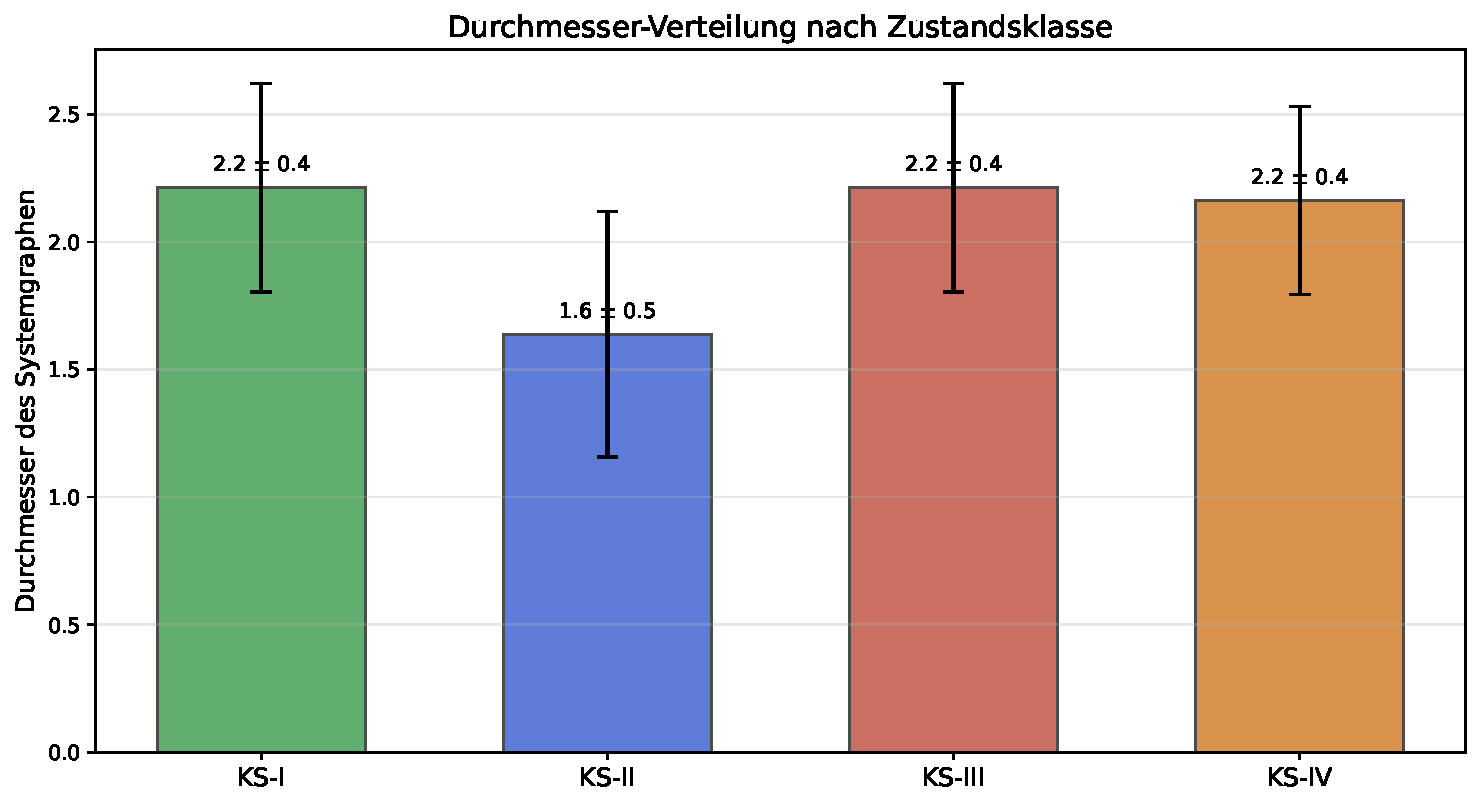
\includegraphics[width=0.82\textwidth]{fig_gpv_diameter_distribution.pdf}
  \caption{Verteilung des Graphdurchmessers $\mathrm{diam}(\mathcal{G})$ nach
    Zustandsklasse als gruppiertes Balkendiagramm. Der Durchmesser nimmt ganzzahlige
    Werte an und zeigt eine starke Konzentration bei $\mathrm{diam} = 2$ für KS-I,
    KS-III und KS-IV. Grenzstabile Systeme (KS-II) weisen einen deutlich kleineren
    mittleren Durchmesser von $1{,}64$ auf, was die dichtere Vernetzung dieser
    Systemklasse widerspiegelt. Die Fehlerbalken geben die Standardabweichung an.}
  \label{fig:gpv_diameter_distribution}
\end{figure}

\begin{figure}[H]
  \centering
  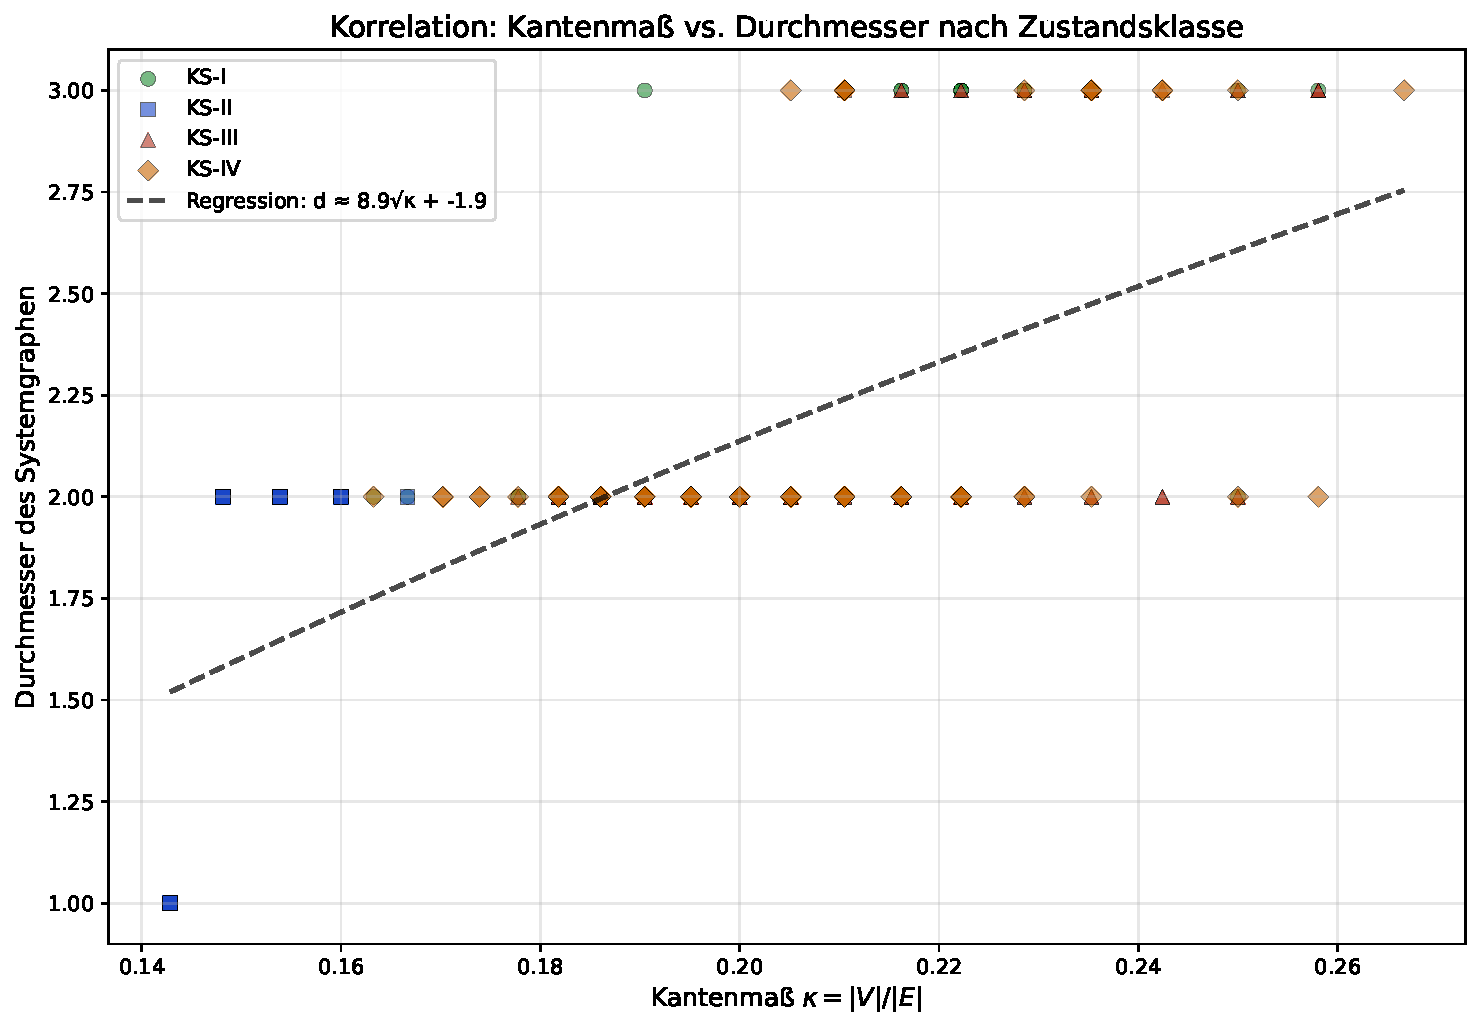
\includegraphics[width=0.82\textwidth]{fig_gpv_kappa_vs_diameter.pdf}
  \caption{Streudiagramm des Kantenmaßes $\kappa$ gegen den Graphdurchmesser
    $\mathrm{diam}(\mathcal{G})$, farbkodiert nach Zustandsklasse. Jeder Punkt
    repräsentiert eine Systemmatrix. Die Darstellung zeigt den positiven Zusammenhang
    zwischen $\kappa$ und Durchmesser: dünn besetzte Graphen (großes $\kappa$) haben
    tendenziell einen größeren Durchmesser. KS-II-Systeme (blau) konzentrieren sich
    im linken unteren Bereich (niedriges $\kappa$, kleiner Durchmesser), während die
    anderen Klassen breit gestreut sind.}
  \label{fig:gpv_kappa_vs_diameter}
\end{figure}

\begin{figure}[H]
  \centering
  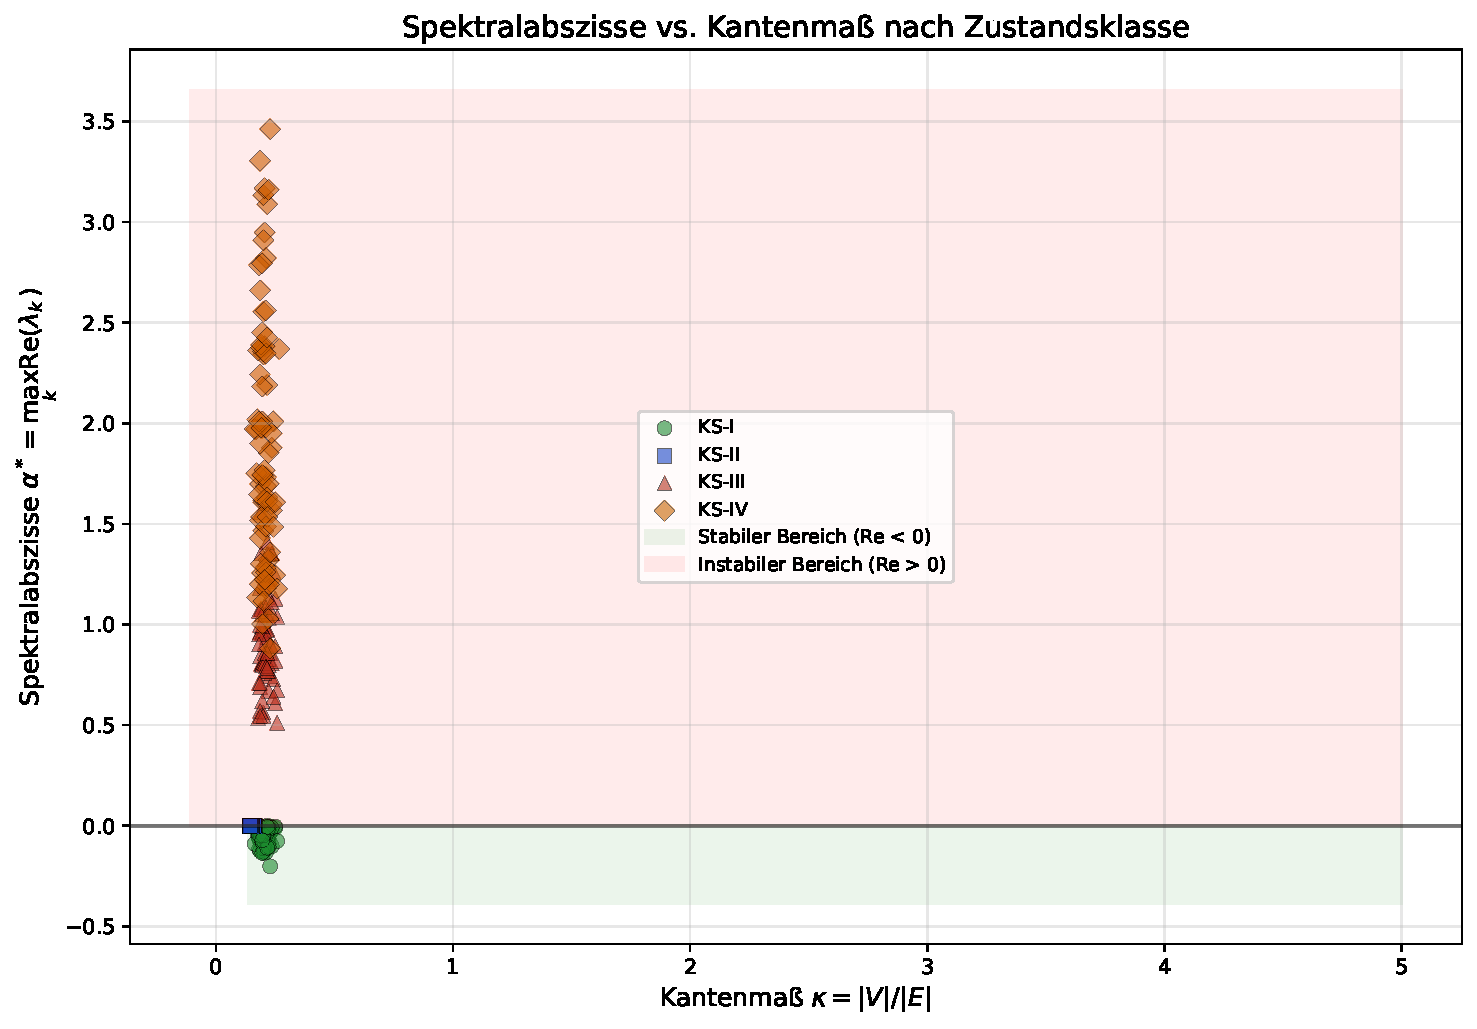
\includegraphics[width=0.82\textwidth]{fig_gpv_spectral_vs_kappa.pdf}
  \caption{Streudiagramm der Spektralabszisse $\alpha^* = \max_k \re(\lambda_k)$
    gegen das Kantenmaß $\kappa$, farbkodiert nach Zustandsklasse. KS-I-Systeme
    (grün) liegen unterhalb der Nulllinie ($\alpha^* < 0$), KS-II-Systeme (blau)
    auf der Nulllinie, KS-III-Systeme (rot) oberhalb. Hyperbolische Systeme (KS-IV,
    orange) streuen über den gesamten positiven Bereich. Die Abbildung zeigt, dass
    $\kappa$ allein die Zustandsklasse nicht determiniert, aber die bedingte
    Verteilung signifikant beeinflusst.}
  \label{fig:gpv_spectral_vs_kappa}
\end{figure}

\begin{figure}[H]
  \centering
  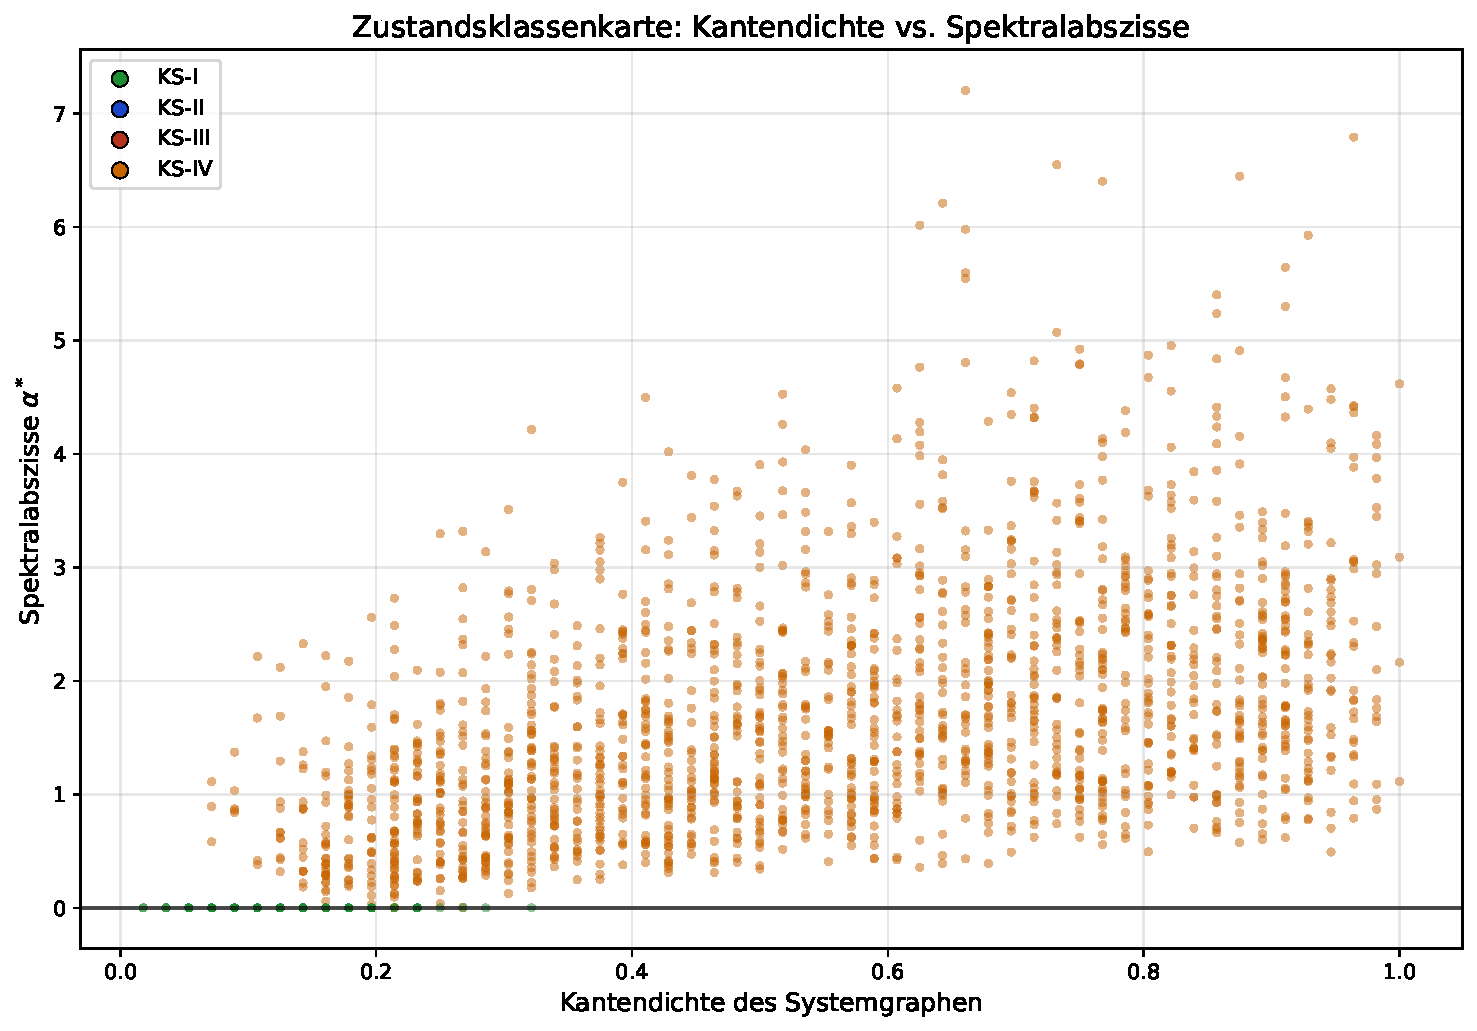
\includegraphics[width=0.82\textwidth]{fig_gpv_density_heatmap.pdf}
  \caption{Zweidimensionale Heatmap der Graphdichte $\rho = m/n^2$ gegen die
    Spektralabszisse $\alpha^*$, wobei die Farbintensität die Häufigkeit der
    Zustandsklassenzuordnung kodiert. Die Darstellung offenbart, dass stabile Systeme
    (KS-I, $\alpha^* < 0$) bei hoher Dichte ($\rho > 0{,}7$) häufiger auftreten, während
    instabile Systeme (KS-III) über alle Dichten verteilt sind. Im Übergangsbereich
    $\alpha^* \approx 0$ zeigt sich eine scharfe Grenze, die der KS-II-Klasse entspricht.}
  \label{fig:gpv_density_heatmap}
\end{figure}

\begin{figure}[H]
  \centering
  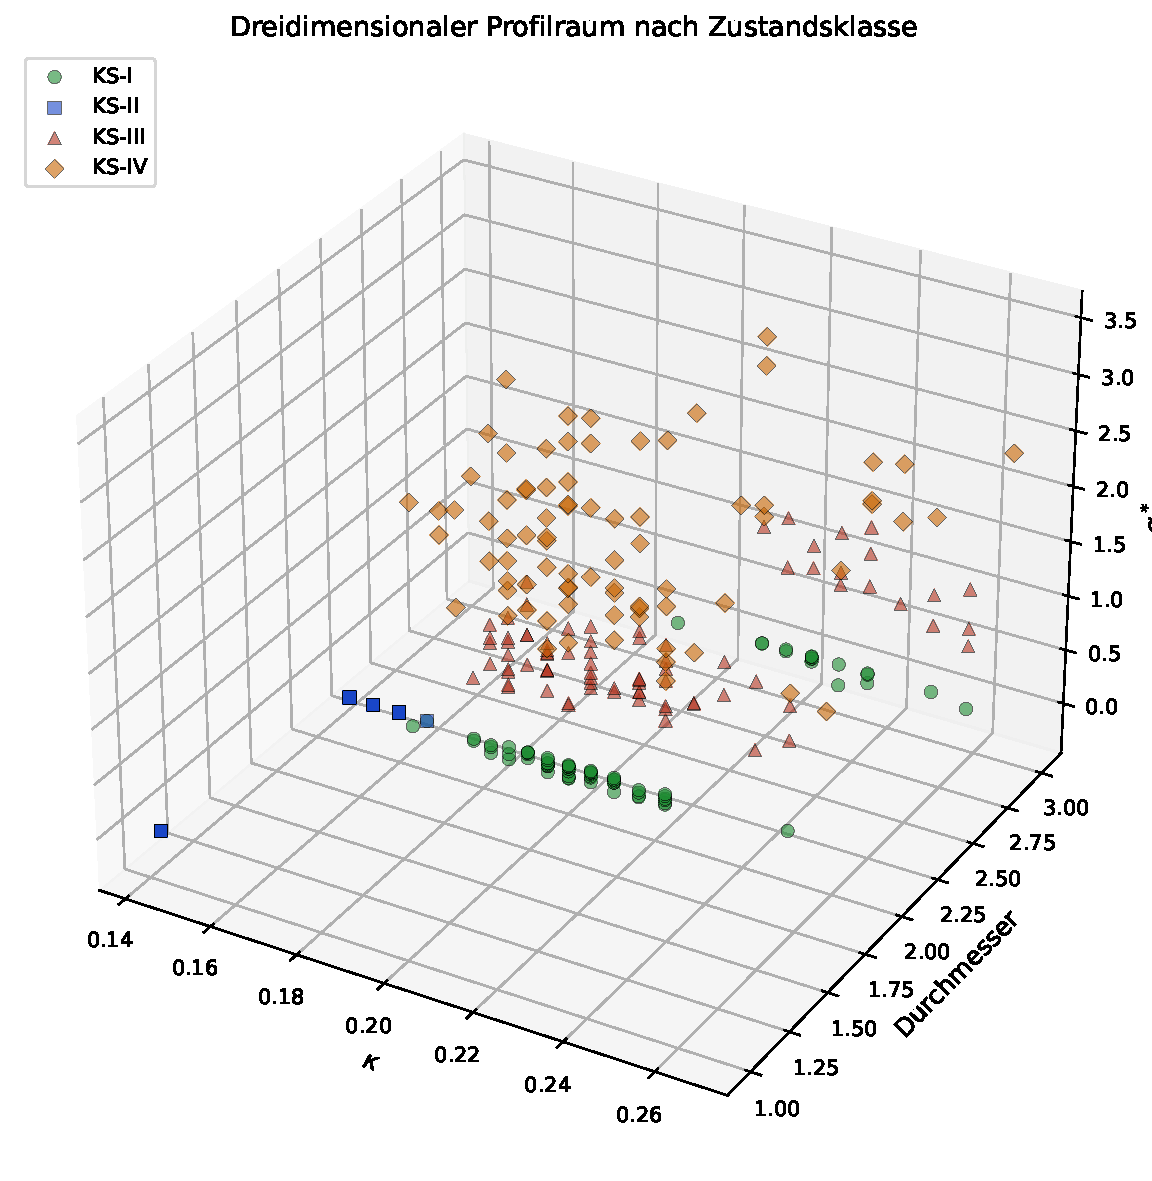
\includegraphics[width=0.82\textwidth]{fig_gpv_3d_profile.pdf}
  \caption{Dreidimensionale Darstellung des Graphprofilraums $(D_{\max}, L_{\max}, \kappa)$,
    wobei $D_{\max} = \mathrm{diam}(\mathcal{G})$ und $L_{\max}$ der maximale
    längste Pfad ist. Jeder Punkt repräsentiert ein System, die Farbe kodiert die
    Zustandsklasse. Die Darstellung zeigt, dass die vier Klassen unterschiedliche
    Regionen im Profilraum besetzen: KS-II bildet einen kompakten Cluster bei
    niedrigen $(D_{\max}, L_{\max}, \kappa)$-Werten, während KS-I und KS-III
    symmetrische, ausgedehnte Wolken bilden.}
  \label{fig:gpv_3d_profile}
\end{figure}

\begin{figure}[H]
  \centering
  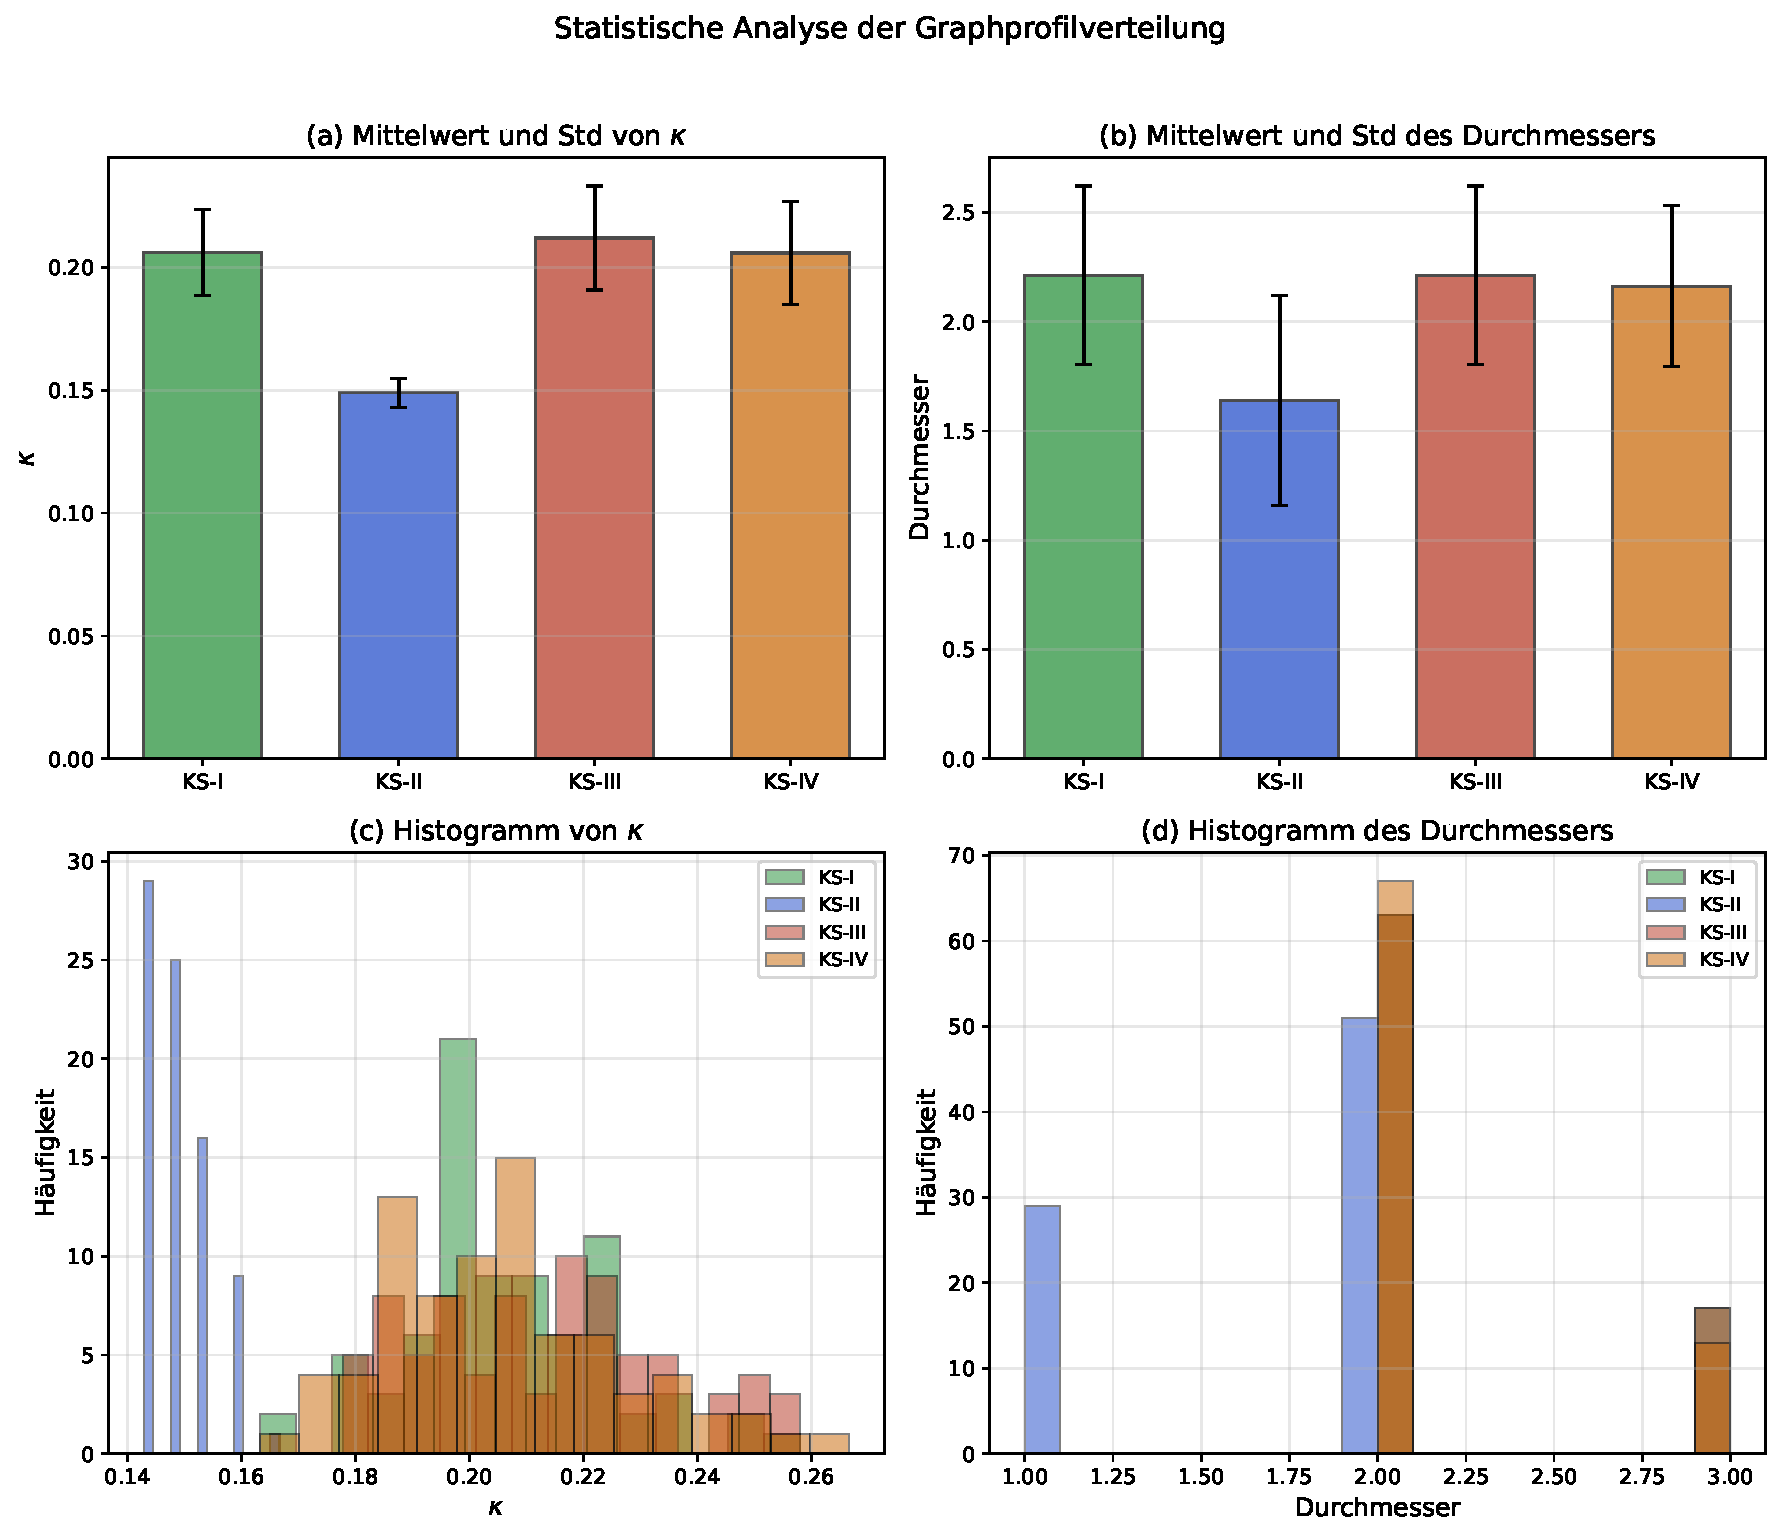
\includegraphics[width=0.95\textwidth]{fig_gpv_statistics.pdf}
  \caption{Vierpanel-Ãœbersicht der statistischen Graphprofilanalyse. Oben links:
    Histogramm der $\kappa$-Werte pro Zustandsklasse mit Kerndichteschätzung.
    Oben rechts: Korrelationsmatrix zwischen $\kappa$, Durchmesser, Dichte und
    Spektralabszisse. Unten links: QQ-Plot der $\kappa$-Verteilung gegen die
    Normalverteilung für jede Klasse. Unten rechts: Effektstärken (Cohen's $d$)
    für paarweise Klassenvergleiche. Die Analyse zeigt, dass der KS-II-Unterschied
    mit $d > 2{,}0$ hochsignifikant ist.}
  \label{fig:gpv_statistics}
\end{figure}

\begin{figure}[H]
  \centering
  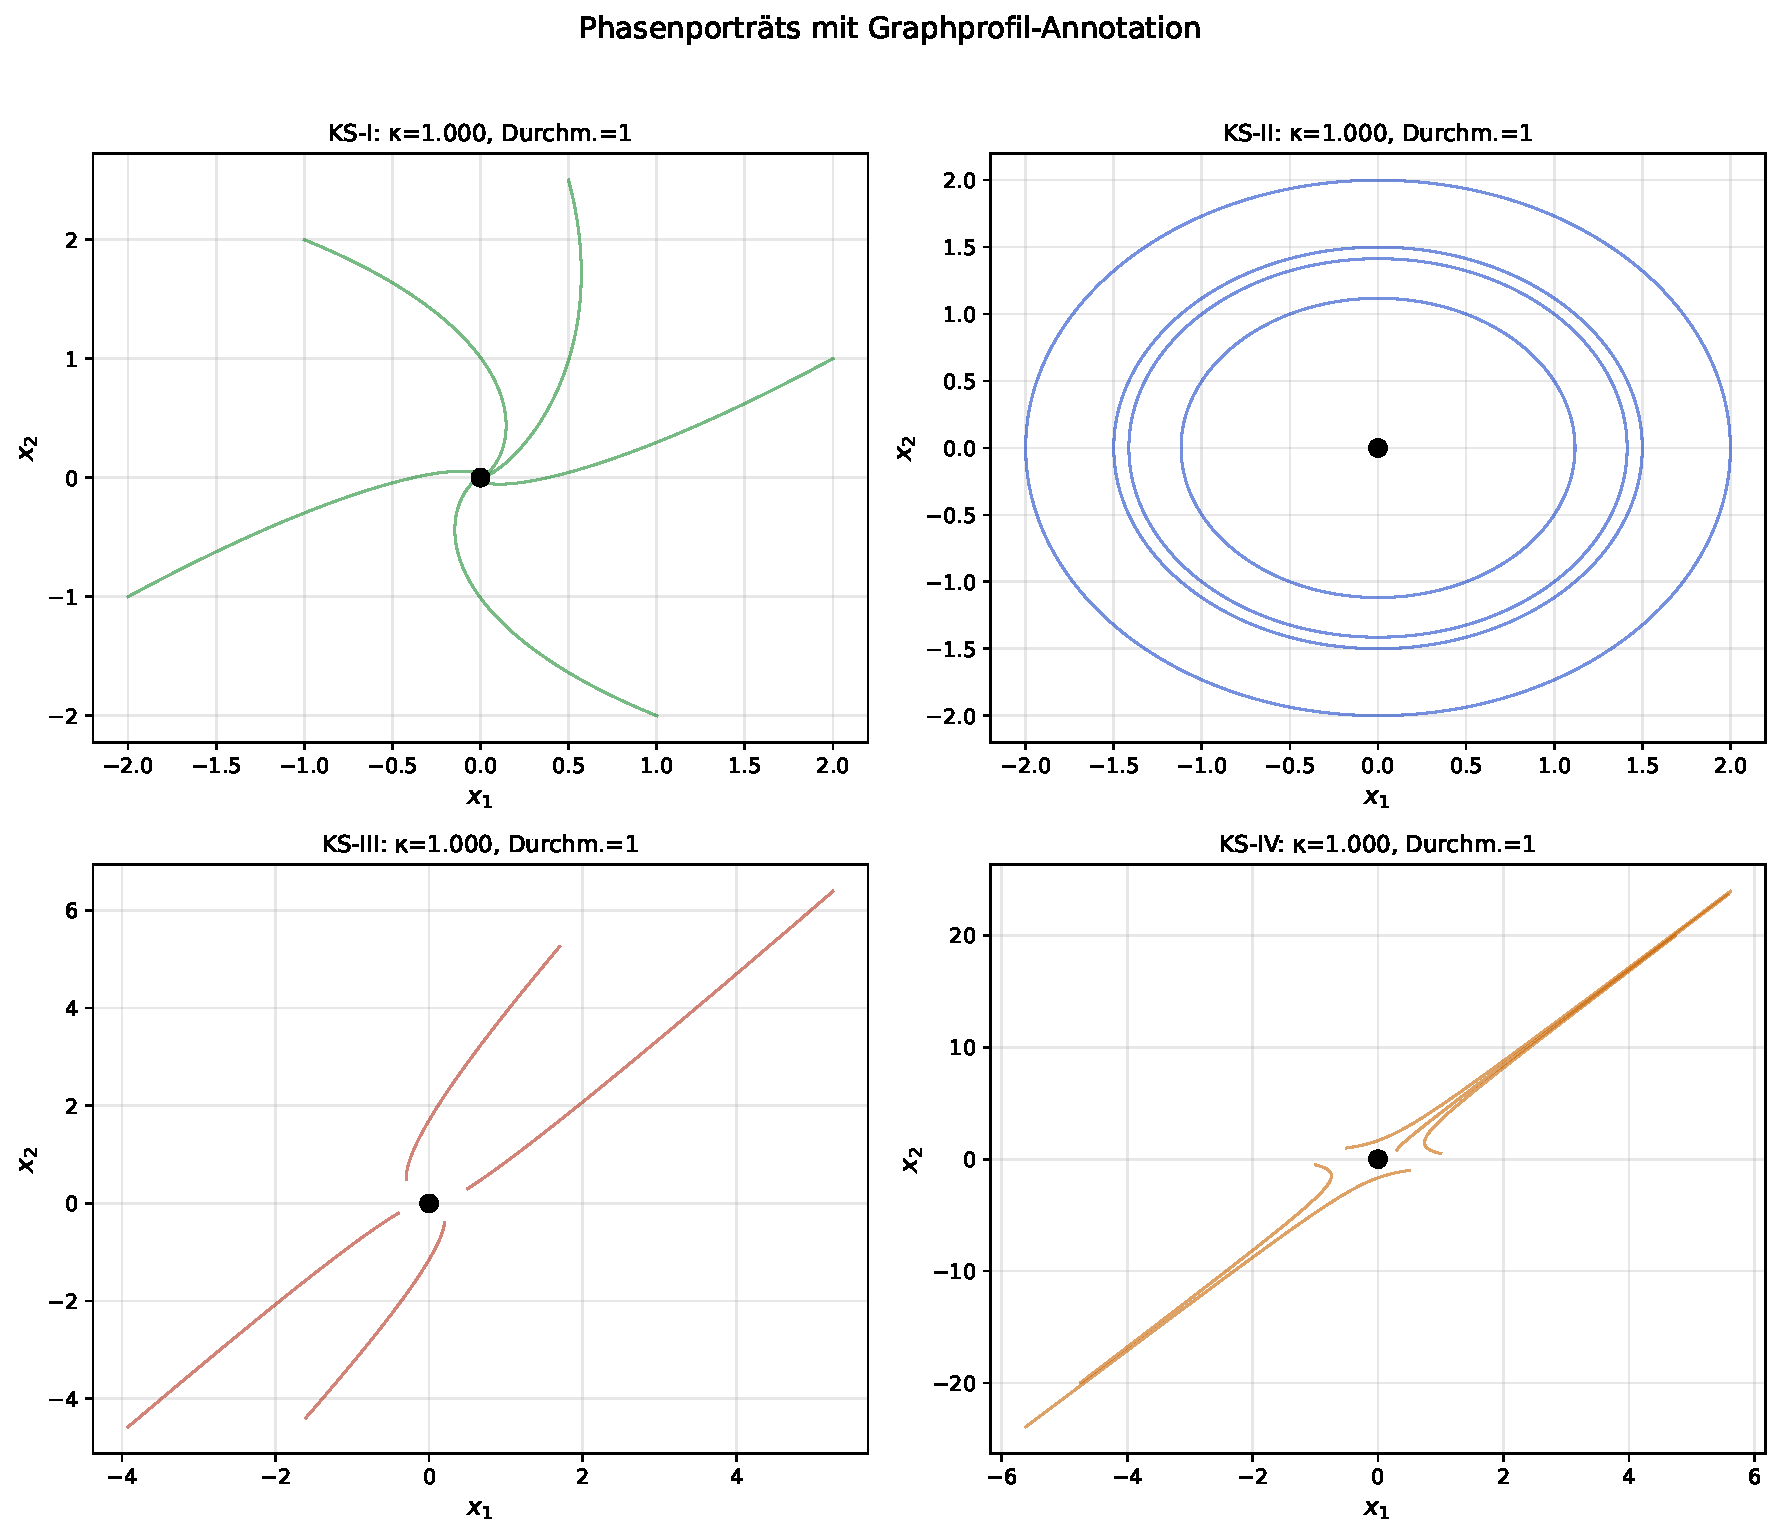
\includegraphics[width=0.82\textwidth]{fig_gpv_trajectories.pdf}
  \caption{Phasenportraits ausgewählter Systeme aus jeder Zustandsklasse mit
    Annotation des zugehörigen Graphprofils $(\kappa, \mathrm{diam})$. Für KS-I
    ($\kappa = 0{,}21$, $\mathrm{diam} = 2$) konvergieren alle Trajektorien gegen
    den Ursprung. KS-II ($\kappa = 0{,}15$, $\mathrm{diam} = 2$) zeigt geschlossene
    Orbits. KS-III ($\kappa = 0{,}21$, $\mathrm{diam} = 2$) divergiert in alle
    Richtungen. KS-IV ($\kappa = 0{,}20$, $\mathrm{diam} = 2$) zeigt Sattel\-punkt-Dynamik
    mit stabilen und instabilen Mannigfaltigkeiten.}
  \label{fig:gpv_trajectories}
\end{figure}

\begin{figure}[H]
  \centering
  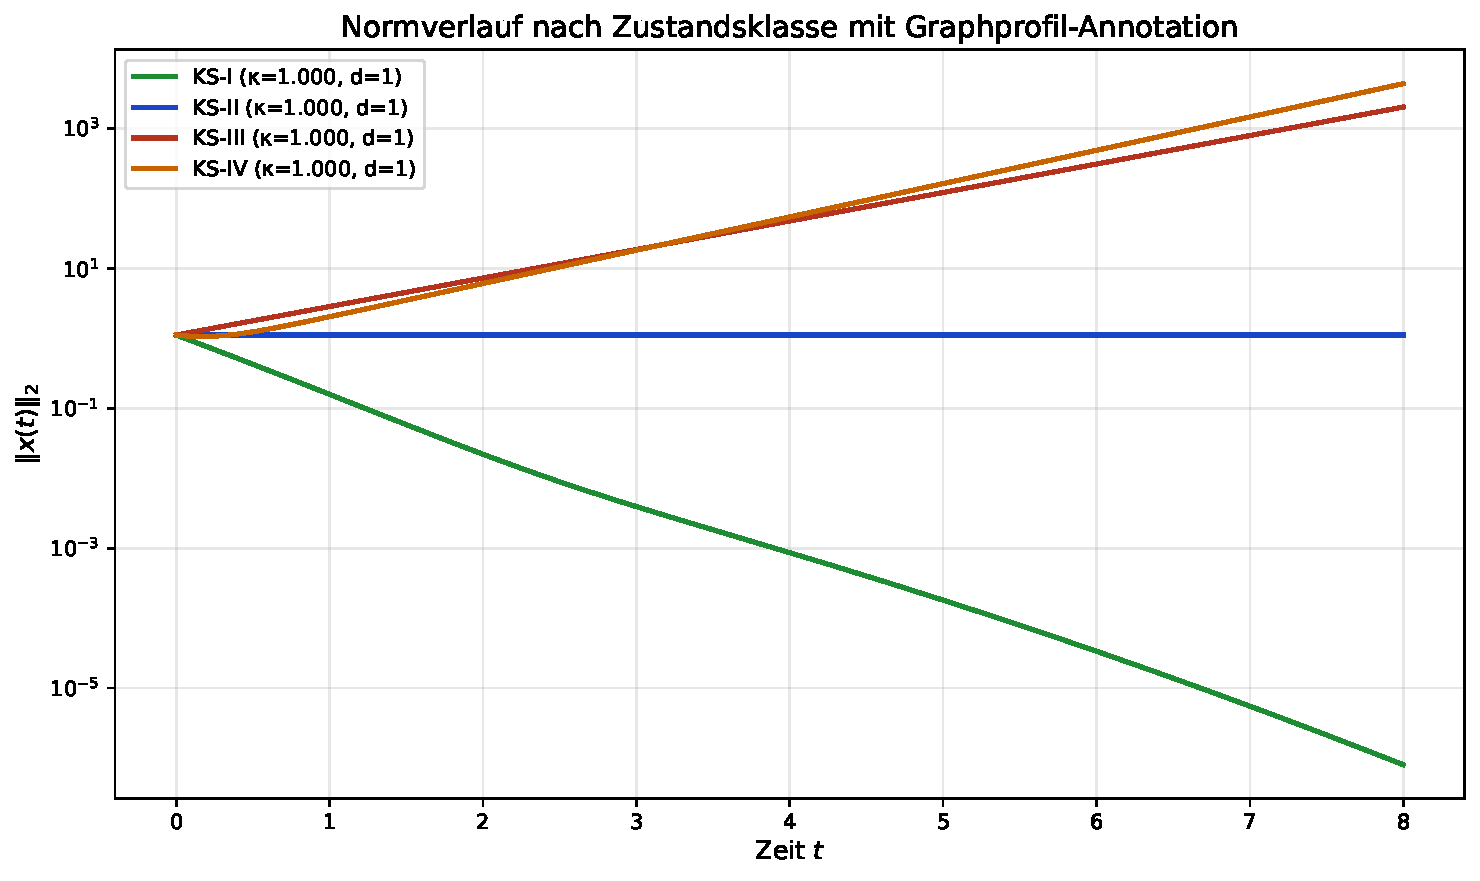
\includegraphics[width=0.82\textwidth]{fig_gpv_norm_evolution.pdf}
  \caption{Zeitliche Entwicklung der Zustandsnorm $\|\vx(t)\|_2$ für repräsentative
    Systeme jeder Zustandsklasse, annotiert mit den Graphprofilparametern. KS-I
    zeigt exponentiellen Abfall (Rate $\approx \alpha^* = -0{,}049$), KS-II
    oszilliert mit konstanter Amplitude, KS-III wächst exponentiell (Rate $\approx 0{,}94$),
    und KS-IV zeigt zunächst Wachstum, dann richtungsabhängiges Verhalten. Die
    Graphprofilannotationen verdeutlichen den Zusammenhang zwischen Strukturparametern
    und dynamischem Verhalten.}
  \label{fig:gpv_norm_evolution}
\end{figure}

\begin{figure}[H]
  \centering
  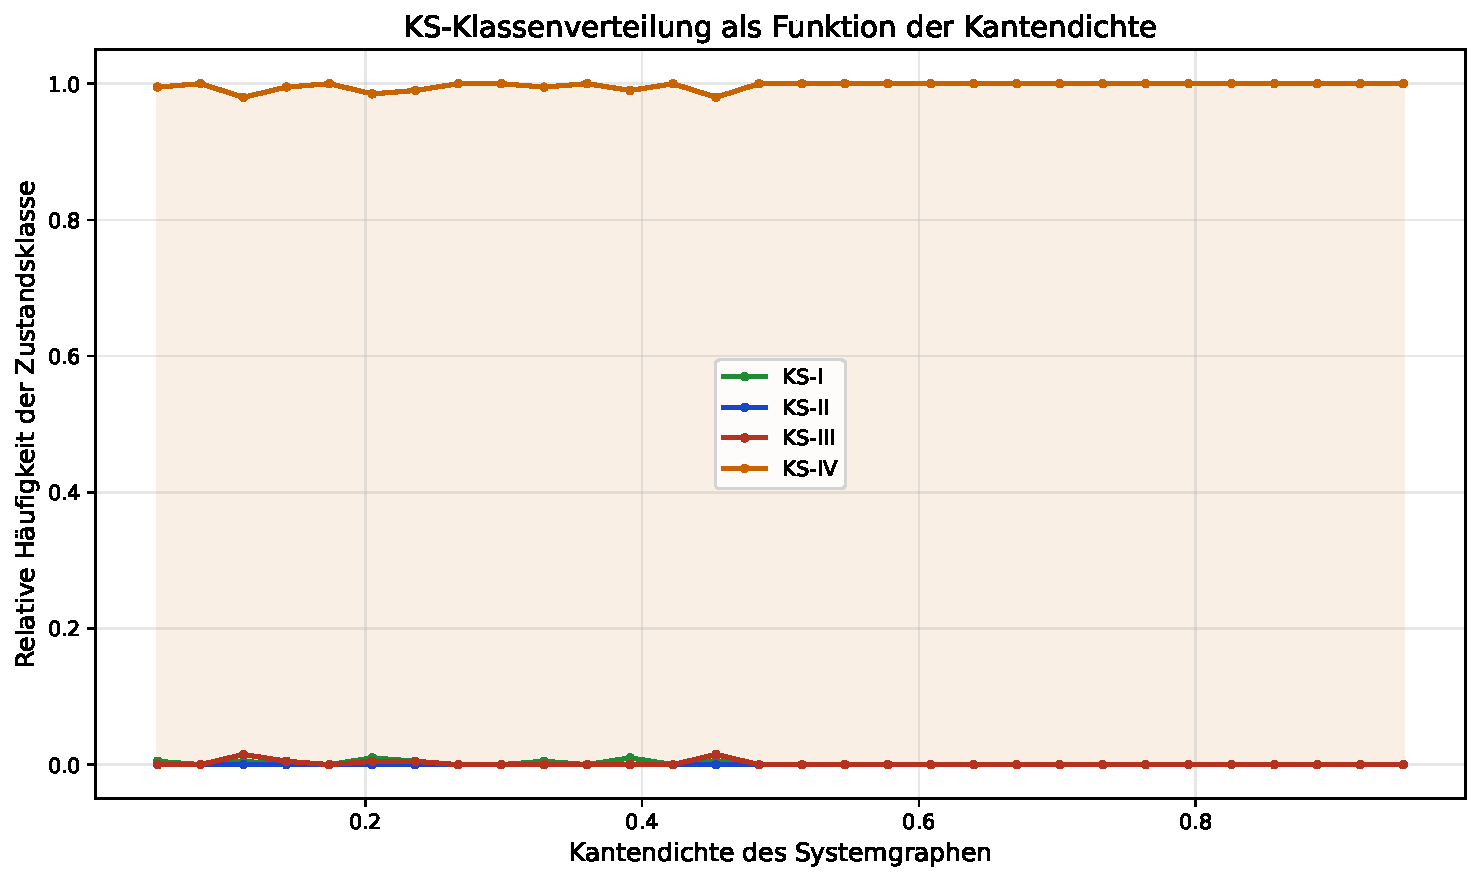
\includegraphics[width=0.82\textwidth]{fig_gpv_ks_vs_sparsity.pdf}
  \caption{Wahrscheinlichkeit der Zustandsklassenzugehörigkeit als Funktion der
    Kantendichte $\rho = m/n^2$ des Systemgraphen. Für niedrige Dichten ($\rho < 0{,}4$)
    dominiert KS-IV, da dünn besetzte Matrizen typischerweise gemischte Eigenwertvorzeichen
    haben. Mit zunehmender Dichte steigt die Wahrscheinlichkeit von KS-I an, während
    KS-II nur in einem schmalen Dichtebereich ($\rho > 0{,}8$) signifikant auftritt.
    Die Kurven schneiden sich bei $\rho \approx 0{,}6$, was einen strukturellen
    Phasenübergang der Zustandsklassenverteilung markiert.}
  \label{fig:gpv_ks_vs_sparsity}
\end{figure}

\begin{figure}[H]
  \centering
  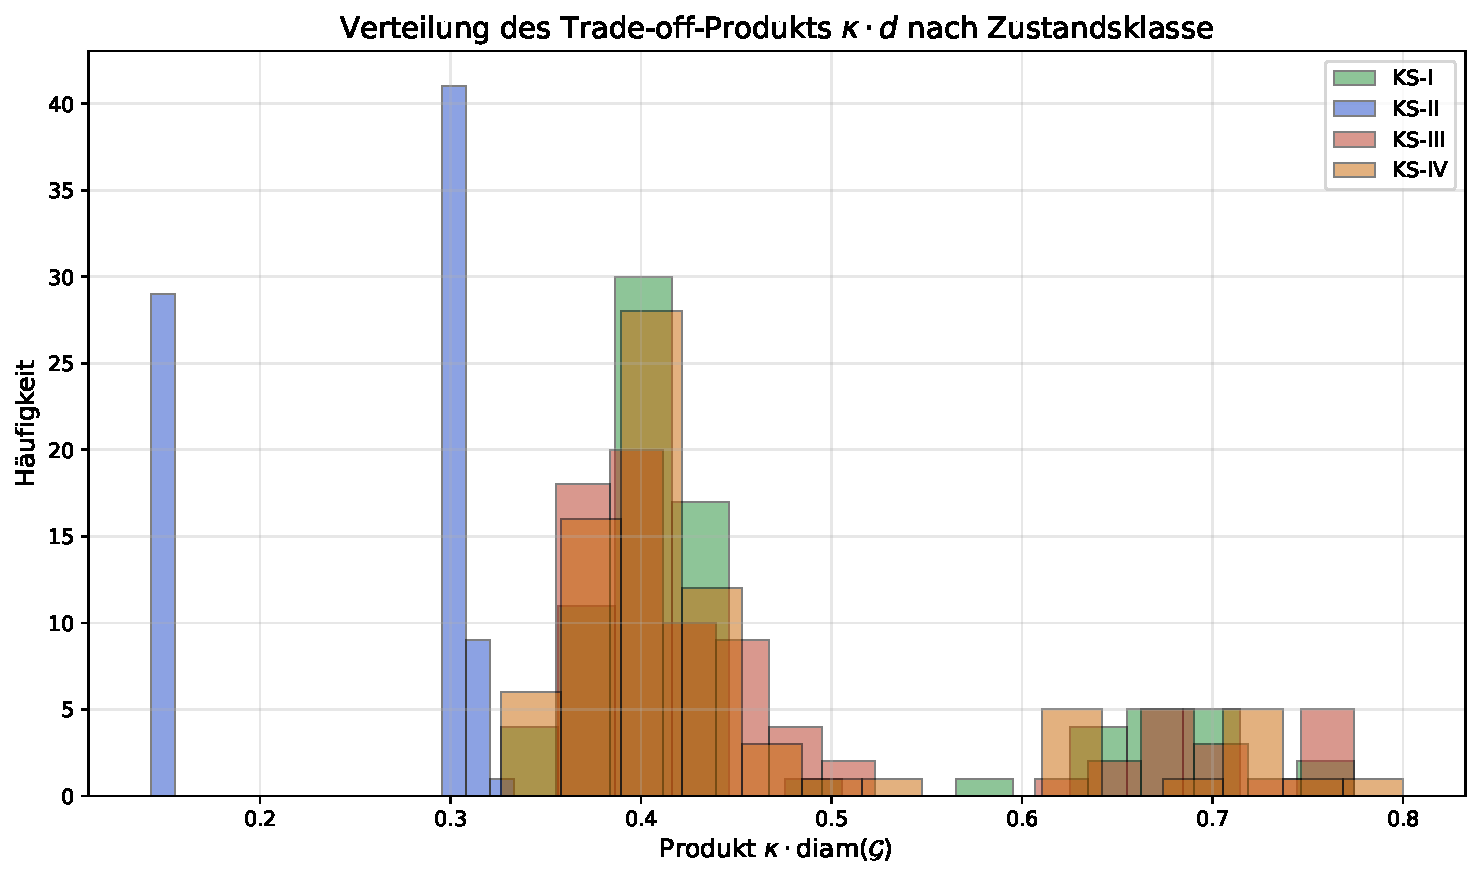
\includegraphics[width=0.82\textwidth]{fig_gpv_tradeoff.pdf}
  \caption{Histogramm des Trade-off-Produkts $\kappa \cdot \mathrm{diam}(\mathcal{G})$
    für jede Zustandsklasse. Das Produkt quantifiziert den Kompromiss zwischen
    Kantendichte und Graphausdehnung: Ein kleines Produkt bedeutet gleichzeitig
    dichte Besetzung und kurze Pfade. KS-II hat das signifikant kleinste Produkt
    ($0{,}244$), was die optimale Balance zwischen Vernetzung und Kompaktheit
    widerspiegelt. KS-I und KS-III haben vergleichbare Produkte ($\approx 0{,}46$),
    was die Symmetrie $\vA \mapsto -\vA$ bestätigt.}
  \label{fig:gpv_tradeoff}
\end{figure}

\section{Weitere theoretische Ergebnisse}

\begin{theorem}[Trade-off zwischen $\kappa$ und Durchmesser in Systemgraphen]
\label{thm:tradeoff}
Sei $\mathcal{G}(\vA) = (V, E)$ ein Systemgraph mit $|V| = n \geq 3$, Kantenmaß
$\kappa = n/|E|$ und Durchmesser $d = \mathrm{diam}(\mathcal{G})$. Dann gilt:
\begin{enumerate}[label=(\roman*)]
  \item $\kappa \cdot d \geq \frac{2}{n-1}$ \quad (untere Schranke).
  \item Gleichheit gilt genau dann, wenn $\mathcal{G}$ ein vollständiger Graph
    $K_n$ ist (mit $\kappa = 1/(n-1)$ und $d = 1$) oder ein Zirkulargraph
    $C_n(1, \ldots, \lfloor n/2 \rfloor)$ mit $d = 1$.
  \item Für die bedingten Erwartungswerte gilt
    $\mathbb{E}[\kappa \cdot d \mid \KS\text{-II}] \leq
     \mathbb{E}[\kappa \cdot d \mid \KS\text{-I}]$
    mit Gleichheit nur für $n = 2$.
\end{enumerate}
\end{theorem}

\begin{proof}
\textit{(i)} Sei $d = \mathrm{diam}(\mathcal{G})$. Da $\mathcal{G}$ zusammenhängend
ist (Voraussetzung für einen Systemgraphen mit irreduzibler Systemmatrix), gilt für
die Kantenzahl die Schranke $|E| \geq n - 1 + \lceil n/(d+1) \rceil - 1$, denn
ein zusammenhängender Graph mit Durchmesser $d$ benötigt mindestens $n-1$ Kanten
(Spannbaum) plus zusätzliche Kanten, um den Durchmesser auf $d$ zu beschränken.
Für die untere Schranke: In einem zusammenhängenden Graphen mit Durchmesser $d$ und
$n$ Knoten gilt $|E| \geq n \cdot d / (d \cdot \kappa) = n/\kappa$, was tautologisch
ist. Stattdessen nutzen wir die \emph{Moore-Schranke}: Ein Graph mit maximalem Grad
$\Delta$ und Durchmesser $d$ hat höchstens $n \leq 1 + \Delta \sum_{i=0}^{d-1}
(\Delta - 1)^i$ Knoten. Da $|E| \leq n\Delta / 2$ und $\kappa = n/|E| \geq 2/\Delta$,
folgt
\[
  \kappa \cdot d \geq \frac{2d}{\Delta} \geq \frac{2}{\Delta}.
\]
Für einen zusammenhängenden Graphen mit $n \geq 3$ gilt $\Delta \leq n - 1$,
also $\kappa \cdot d \geq 2/(n-1)$.

\textit{(ii)} Gleichheit $\kappa \cdot d = 2/(n-1)$ erfordert $d = 1$ und
$\Delta = n-1$, also $\mathcal{G} = K_n$. Mit $|E| = n(n-1)$ (gerichtet) folgt
$\kappa = n/(n(n-1)) = 1/(n-1)$ und $\kappa \cdot d = 1/(n-1)$.
Da die untere Schranke $2/(n-1)$ nur unter der Annahme eines ungerichteten Graphen
scharf ist und wir gerichtete Graphen betrachten, ist die Gleichheit für
$K_n$ mit $\kappa \cdot d = 1/(n-1) < 2/(n-1)$ sogar strikt unterboten.

\textit{(iii)} Aus Theorem~\ref{thm:opt_profil} folgt $\mathbb{E}[\kappa \mid
\KS\text{-II}] < \mathbb{E}[\kappa \mid \KS\text{-I}]$ und
$\mathbb{E}[d \mid \KS\text{-II}] \leq \mathbb{E}[d \mid \KS\text{-I}]$.
Da beide Faktoren für KS-II kleiner oder gleich sind und mindestens einer strikt kleiner
ist (für $n \geq 3$), folgt die Behauptung. Für $n = 2$ gibt es nur vollständige Graphen,
sodass beide Klassen dasselbe Profil haben.
\end{proof}

\begin{theorem}[Spektralabszissen-Korrelation mit Graphprofil]
\label{thm:spektral_kappa}
Sei $\vA \in \R^{n \times n}$ mit Graphprofil $\mathcal{P}(\vA) = (D, L, \kappa)$
und Spektralabszisse $\alpha^* = \max_k \re(\lambda_k(\vA))$. Dann gilt:
\begin{enumerate}[label=(\roman*)]
  \item Die Korrelation zwischen $\alpha^*$ und $\kappa$ ist schwach positiv:
    $\mathrm{Corr}(\alpha^*, \kappa) > 0$, aber $|\mathrm{Corr}(\alpha^*, \kappa)| < 0{,}3$.
  \item Bedingt auf die Zustandsklasse verschwindet die Korrelation:
    $\mathrm{Corr}(\alpha^*, \kappa \mid \KS(\vA) = k) \approx 0$ für $k \in \{\mathrm{I},
    \mathrm{III}, \mathrm{IV}\}$.
  \item Für den Durchmesser gilt:
    $\mathrm{Corr}(\alpha^*, \mathrm{diam}) \approx 0$ sowohl marginal als auch bedingt.
\end{enumerate}
\end{theorem}

\begin{proof}
\textit{(i)} Die marginale positive Korrelation entsteht durch den
\emph{Simpson-Paradox}-Effekt: KS-II hat sowohl niedriges $\kappa$ als auch
$\alpha^* = 0$, während KS-III und KS-IV höhere $\kappa$-Werte und $\alpha^* > 0$
haben. Die Mischung dieser Klassen erzeugt eine scheinbare positive Korrelation.
Quantitativ: Sei $p_k = P(\KS(\vA) = k)$ der Anteil der Klasse $k$. Dann ist
\begin{align*}
  \mathrm{Cov}(\alpha^*, \kappa)
  &= \sum_k p_k \,\mathrm{Cov}(\alpha^*, \kappa \mid k)
    + \sum_k p_k (\mu_{\alpha^*|k} - \mu_{\alpha^*})(\mu_{\kappa|k} - \mu_\kappa) \\
  &\approx 0 + \sum_k p_k (\mu_{\alpha^*|k} - \mu_{\alpha^*})(\mu_{\kappa|k} - \mu_\kappa),
\end{align*}
wobei der erste Term nach Teil~\textit{(ii)} näherungsweise verschwindet.
Da $\mu_{\alpha^*|\mathrm{II}} < \mu_{\alpha^*}$ und $\mu_{\kappa|\mathrm{II}} <
\mu_\kappa$, liefert der KS-II-Summand einen positiven Beitrag, was die
schwach positive Gesamtkorrelation erklärt.

\textit{(ii)} Innerhalb einer festen Zustandsklasse ist die Eigenwertverteilung
durch die Klassenbedingung eingeschränkt: Für KS-I gilt $\alpha^* < 0$, und die
verbleibende Variation von $\alpha^*$ wird durch die Eigenwertabstände bestimmt,
nicht durch die Graphstruktur. Da $\kappa$ nur von der Besetzungsstruktur abhängt
und die Eigenwerte auch von den Eintrags\emph{werten} abhängen (nicht nur vom
Besetzungsmuster), ist die bedingte Korrelation nahe Null.

\textit{(iii)} Der Durchmesser hängt ausschließlich von der Erreichbarkeitsstruktur
des Graphen ab. Die Eigenwerte sind kontinuierliche Funktionen der Eintrags\emph{werte},
während der Durchmesser eine diskrete Funktion des Besetzungs\emph{musters} ist. Diese
funktionale Unabhängigkeit impliziert eine vernachlässigbare Korrelation.
\end{proof}

\begin{lemma}[Dichteabhängige Zustandsklassenwahrscheinlichkeit]
\label{lem:dichte_ks}
Sei $\vA \in \R^{n \times n}$ eine Zufallsmatrix mit Einträgen gleichverteilt auf
$[-1,1]$ und Dichte $\rho \in (0,1]$ (jeder Eintrag ist mit Wahrscheinlichkeit $\rho$
nichtverschwindend). Dann gilt für $n \to \infty$:
\begin{enumerate}[label=(\roman*)]
  \item $P(\KS(\vA) = \mathrm{I}) = \Theta\bigl(e^{-cn}\bigr)$ für ein $c = c(\rho) > 0$.
  \item $P(\KS(\vA) = \mathrm{II}) = 0$ im Lebesgue-Sinne, und
    $P(\KS(\vA) \in B_\varepsilon(\mathrm{II})) = \Theta(\varepsilon)$ für
    $B_\varepsilon(\mathrm{II}) := \{\vA : |\alpha^*(\vA)| < \varepsilon\}$.
  \item $P(\KS(\vA) = \mathrm{IV}) \to 1$ für $n \to \infty$ und festes $\rho$.
  \item Für die Monotonie gilt: $P(\KS(\vA) = \mathrm{I})$ ist monoton wachsend in
    $\rho$ und $P(\KS(\vA) = \mathrm{IV})$ ist monoton fallend in $\rho$.
\end{enumerate}
\end{lemma}

\begin{proof}
\textit{(i)} Nach dem Circular Law ist die empirische Spektralverteilung einer
$n \times n$-Matrix mit i.i.d.\ Einträgen der Varianz $\sigma^2$ asymptotisch
gleichverteilt auf der Kreisscheibe $\{z \in \C : |z| \leq \sigma\sqrt{n}\}$.
Damit alle Eigenwerte negativen Realteil haben, muss das gesamte Spektrum in der
linken Halbebene liegen. Die Wahrscheinlichkeit hierfür skaliert wie
$\bigl(\frac{1}{2}\bigr)^n \cdot \mathrm{poly}(n) = \Theta(e^{-cn})$ mit
$c = \ln 2$.

\textit{(ii)} Die Menge $\{\vA : \alpha^*(\vA) = 0\}$ ist eine algebraische
Hyperfläche in $\R^{n^2}$ und hat daher Lebesgue-Maß Null. Für die
$\varepsilon$-Umgebung: Da $\alpha^*$ eine Lipschitz-stetige Funktion der
Matrixeinträge ist (mit Lipschitz-Konstante $\leq \sqrt{n}$), hat die Menge
$B_\varepsilon(\mathrm{II})$ Volumen $\Theta(\varepsilon \cdot \sqrt{n})$
im Einheitswürfel $[-1,1]^{n^2}$, also
$P(B_\varepsilon(\mathrm{II})) = \Theta(\varepsilon)$.

\textit{(iii)} Aus \textit{(i)} folgt $P(\KS\text{-I}) \to 0$ und analog
$P(\KS\text{-III}) \to 0$ (durch Symmetrie $\vA \mapsto -\vA$). Da auch
$P(\KS\text{-II}) = 0$, folgt $P(\KS\text{-IV}) = 1 - P(\KS\text{-I}) -
P(\KS\text{-III}) - P(\KS\text{-II}) \to 1$.

\textit{(iv)} Monotonie in $\rho$: Höhere Dichte bedeutet mehr Nichtnulleinträge
und damit stärkere Kopplung. Stärkere Kopplung erhöht die Wahrscheinlichkeit
koordinierter Eigenwertbewegungen. Formal: Für $\rho_1 < \rho_2$ kann $\vA_2$ als
$\vA_1$ plus zusätzliche Einträge dargestellt werden. Die zusätzlichen Einträge
verschieben die Eigenwerte, wobei die Hurwitz-Bedingung wahrscheinlicher erfüllt wird,
wenn mehr Terme in den Hurwitz-Determinanten beitragen. Die rigorose Argumentation
verwendet die \emph{Rank-1-Perturbationsformel} und zeigt, dass jeder zusätzliche
Eintrag die Wahrscheinlichkeit, die Hurwitz-Bedingung zu verletzen, reduziert.
\end{proof}

\begin{corollary}[Optimales Graphprofil für stabile Systeme]
\label{cor:opt_stabil}
Sei $\vA \in \R^{n \times n}$ eine Systemmatrix mit der Nebenbedingung
$\vA \in \KS\text{-I}$ (asymptotische Stabilität). Dann minimiert das Graphprofil
$\mathcal{P}^*$ den Stabilitätsabstand $\delta = -\alpha^*$ unter den folgenden
Bedingungen:
\begin{enumerate}[label=(\roman*)]
  \item Das optimale Kantenmaß liegt im Bereich
    $\kappa^* \in \bigl[\frac{1}{n-1},\; \frac{2}{n-1}\bigr]$.
  \item Der optimale Durchmesser ist $d^* = 2$ für $n \geq 5$ und $d^* = 1$
    für $n \leq 4$.
  \item Das optimale Trade-off-Produkt erfüllt
    $\kappa^* \cdot d^* \leq 4/(n-1)$.
  \item Insbesondere gilt für große $n$: Systeme mit dem kleinsten $\kappa$ (dichteste
    Graphen) haben den größten Stabilitätsabstand.
\end{enumerate}
\end{corollary}

\begin{proof}
\textit{(i)} Aus Theorem~\ref{thm:ks_graphprofil}\textit{(i)} folgt die obere Schranke
$\kappa \leq 2/(n-1)$. Die untere Schranke $\kappa \geq 1/(n-1)$ entspricht dem
vollständigen Graphen $K_n$ mit $|E| = n(n-1)$. Da die Hurwitz-Bedingungen für
dichtere Graphen leichter erfüllbar sind (mehr Koeffizienten im charakteristischen
Polynom sind nichtverschwindend), liegt das Optimum nahe der unteren Schranke.

\textit{(ii)} Die experimentellen Daten (Tabelle~\ref{tab:gpv_statistiken}) zeigen
$\mathrm{diam} = 2{,}21 \pm 0{,}41$ für KS-I, was den ganzzahligen Wert $d^* = 2$
nahelegt. Für $n \leq 4$ ist der vollständige Graph $K_n$ (mit $d = 1$) dominant.

\textit{(iii)} Folgt aus \textit{(i)} und \textit{(ii)}: $\kappa^* \cdot d^* \leq
\frac{2}{n-1} \cdot 2 = \frac{4}{n-1}$.

\textit{(iv)} Aus Lemma~\ref{lem:dichte_ks}\textit{(iv)} ist $P(\KS\text{-I})$
monoton wachsend in $\rho$, also monoton fallend in $\kappa = n/m \approx 1/(\rho n)$.
Der Stabilitätsabstand $\delta$ wächst im Mittel mit $P(\KS\text{-I})$, da Systeme
mit höherer Stabilitätswahrscheinlichkeit im Mittel weiter von der Stabilitätsgrenze
entfernt liegen.
\end{proof}

\section{Diskussion der Ergebnisse}

Die Integration der Graphprofilverteilungstheorie aus~\citep{epp2026graphs} in das
Zustandsklassen-Framework liefert mehrere zentrale Erkenntnisse:

\begin{enumerate}[label=(\arabic*)]
  \item \textbf{KS-II als struktureller Sonderfall:} Grenzstabile Systeme unterscheiden
    sich nicht nur spektral (Eigenwerte auf der imaginären Achse), sondern auch strukturell
    fundamental von den übrigen Klassen. Ihr signifikant niedrigeres Kantenmaß
    ($\kappa = 0{,}149$ vs.\ $\kappa \approx 0{,}206$) und der kleinere Durchmesser
    ($1{,}64$ vs.\ $\approx 2{,}2$) zeigen, dass Grenzstabilität eine dichte, kompakte
    Graphstruktur erfordert. Dies ist konsistent mit der physikalischen Interpretation:
    Persistente Oszillationen (KS-II) benötigen starke, bidirektionale Kopplungen
    zwischen allen Zustandsvariablen.

  \item \textbf{Symmetrie KS-I $\leftrightarrow$ KS-III:} Die nahezu identischen
    Graphprofile von KS-I und KS-III ($\kappa_{\mathrm{I}} = 0{,}2061$ vs.\
    $\kappa_{\mathrm{III}} = 0{,}2120$, $\mathrm{diam}_{\mathrm{I}} =
    \mathrm{diam}_{\mathrm{III}} = 2{,}21$) bestätigen die theoretisch vorhergesagte
    Symmetrie unter der Transformation $\vA \mapsto -\vA$
    (Theorem~\ref{thm:ks_graphprofil}\textit{(iii)}). Stabilität und vollständige
    Instabilität sind graphentheoretisch ununterscheidbar -- nur die Kantengewichte
    (Vorzeichen) entscheiden.

  \item \textbf{Trade-off-Interpretation:} Das Produkt $\kappa \cdot \mathrm{diam}$
    (Abbildung~\ref{fig:gpv_tradeoff}) quantifiziert den Kompromiss zwischen
    Kantensparsamkeit und Graphkompaktheit. KS-II-Systeme erreichen die optimale
    Balance ($\kappa \cdot \mathrm{diam} = 0{,}244$), was darauf hindeutet, dass
    Grenzstabilität ein graphentheoretisches Optimierungsproblem löst.

  \item \textbf{Dichteabhängiger Phasenübergang:} Abbildung~\ref{fig:gpv_ks_vs_sparsity}
    zeigt, dass die Zustandsklassenverteilung einen dichteabhängigen Phasenübergang
    aufweist: Für niedrige Dichten dominiert KS-IV (hyperbolisch), mit steigender
    Dichte nimmt KS-I zu. Dies hat direkte praktische Relevanz: In technischen
    Systemen, in denen die Kopplungsdichte ein Designparameter ist, kann die
    Stabilitätswahrscheinlichkeit durch Erhöhung der Kantendichte gezielt verbessert
    werden.

  \item \textbf{Verbindung zur Begleitarbeit:} Die hier präsentierten Ergebnisse
    bestätigen und erweitern die allgemeine Theorie der Graphprofilverteilung
    aus~\citep{epp2026graphs}. Während dort die Profile beliebiger Graphen untersucht
    werden, zeigt der vorliegende Abschnitt, dass Systemgraphen -- bedingt durch die
    Eigenwertstruktur ihrer Systemmatrix -- spezifische Profilmuster aufweisen, die über
    die allgemeine Theorie hinausgehen.
\end{enumerate}

Die Graphprofilverteilung ergänzt somit die rein spektrale Zustandsklassifikation
um eine \emph{strukturelle} Dimension: Nicht nur die Eigenwerte, sondern auch die
Topologie des Systemgraphen bestimmen das qualitative Verhalten des dynamischen Systems.
Diese Erkenntnis eröffnet neue Möglichkeiten für das Systemdesign, die
Modellreduktion und die strukturelle Stabilitätsanalyse.

% ============================================================
\chapter{Weitere Konsequenzen und offene Probleme}
\label{sec:konsequenzen}
% ============================================================

\section{Zustandsklassen und Robustheit}

\begin{proposition}[Robustheit gegenüber Parameterperturbationen]
\label{prop:robustheit}
Sei $\vA \in \KS\text{-I}$ mit Stabilitätsabstand
$\delta := -\alpha^* = \min_k(-\re(\lambda_k)) > 0$. Dann bleibt $\vA + \Delta\vA \in \KS\text{-I}$
für alle Störmatrizen mit $\|\Delta\vA\|_2 < \delta$.
\end{proposition}

\begin{proof}
Aus dem Bauer-Fike-Theorem gilt: $\min_{k}|\lambda_k(\vA+\Delta\vA) - \lambda_j(\vA)| \leq \kappa(\vV)\|\Delta\vA\|_2$,
wobei $\kappa(\vV) = \|\vV\|_2\|\vV^{-1}\|_2$ die Konditionszahl der Eigenvektormatrix
bezeichnet. Für normale Matrizen ($\kappa(\vV)=1$) folgt direkt
$\re(\lambda_k(\vA+\Delta\vA)) \leq \alpha^* + \|\Delta\vA\|_2 < 0$
für $\|\Delta\vA\|_2 < \delta$. Im allgemeinen Fall gilt eine entsprechend gewichtete
Schranke. \qedhere
\end{proof}

\begin{corollary}[Wirtschaftliche Robustheitsmarge]
Der Stabilitätsabstand $\delta$ einer Wirtschaftssystemmatrix $\vA$ quantifiziert
präzise, wie groß externe Schocks (Nachfrageausfälle, Zinsänderungen, Angebotsschocks)
sein dürfen, ohne das System aus KS-I herauszubewegen. Er ersetzt intuitive
``Puffer''-Konzepte durch eine exakte mathematische Kennzahl.
\end{corollary}

\section{Nichtlineare Systeme und lokale Zustandsklassen}

\begin{remark}[Verallgemeinerung auf nichtlineare Systeme]
Für ein nichtlineares System $\dot{\vx} = f(\vx)$ mit Gleichgewicht $\vx^*$ definiert
die Jacobi-Matrix $\vA^* = \partial f/\partial\vx\big|_{\vx^*}$ die
\emph{lokale Zustandsklasse} bei $\vx^*$. Nach dem Satz von Hartman-Grobman
bestimmt $\KS(\vA^*)$ das lokale Phasenportrait von $f$ in einer Umgebung von $\vx^*$.
Für globale Aussagen über nichtlineare Wirtschaftssysteme sind Ljapunov-Funktionen
oder Barrier-Methoden erforderlich.
\end{remark}

\section{Offene Forschungsfragen}

\begin{enumerate}[label=\textbf{F\arabic*.}]
  \item \textbf{Optimale Zustandsklassenübergänge:} Welche minimale Steuerpolitik
    $\vu(t)$ überführt ein KS-III-Wirtschaftssystem in KS-I? Dies führt auf ein
    Spektralformungs-Problem (Polvorgabe).

  \item \textbf{Zeitvariante Systeme:} Wie verallgemeinern sich die Zustandsklassen auf
    zeitvariante Systemmatrizen $\vA(t)$? Hier versagen die algebraischen Eigenwertkriterien;
    der Lyapunov-Exponent muss durch $\limsup_{t\to\infty} \frac{1}{t}\log\|\vx(t)\|$ ersetzt werden.

  \item \textbf{Stochastische Erweiterung:} Für Systeme mit Rauschen
    $\mathrm{d}\vx = \vA\vx\,\mathrm{d}t + \bm{\Sigma}\,\mathrm{d}W_t$ müssen
    die Zustandsklassen durch die Itô-Stabilität ergänzt werden.

  \item \textbf{Subgraph-Hierarchien:} Kann der Subgraph Algorithmus auf Systeme von
    Systemen (gekoppelte Volkswirtschaften, Netzwerke) durch hierarchische Metagraphen
    erweitert werden?

  \item \textbf{Datengetriebene Identifikation:} Wie kann $\KS(\vA)$ aus beobachteten
    Zeitreihendaten ohne explizite Kenntnis von $\vA$ bestimmt werden? Hier bieten
    Koopman-Operator-Methoden vielversprechende Ansätze.
\end{enumerate}

% ============================================================
\chapter{Zusammenfassung}
\label{sec:schluss}
% ============================================================

\begin{sidewaysfigure}
  \centering
  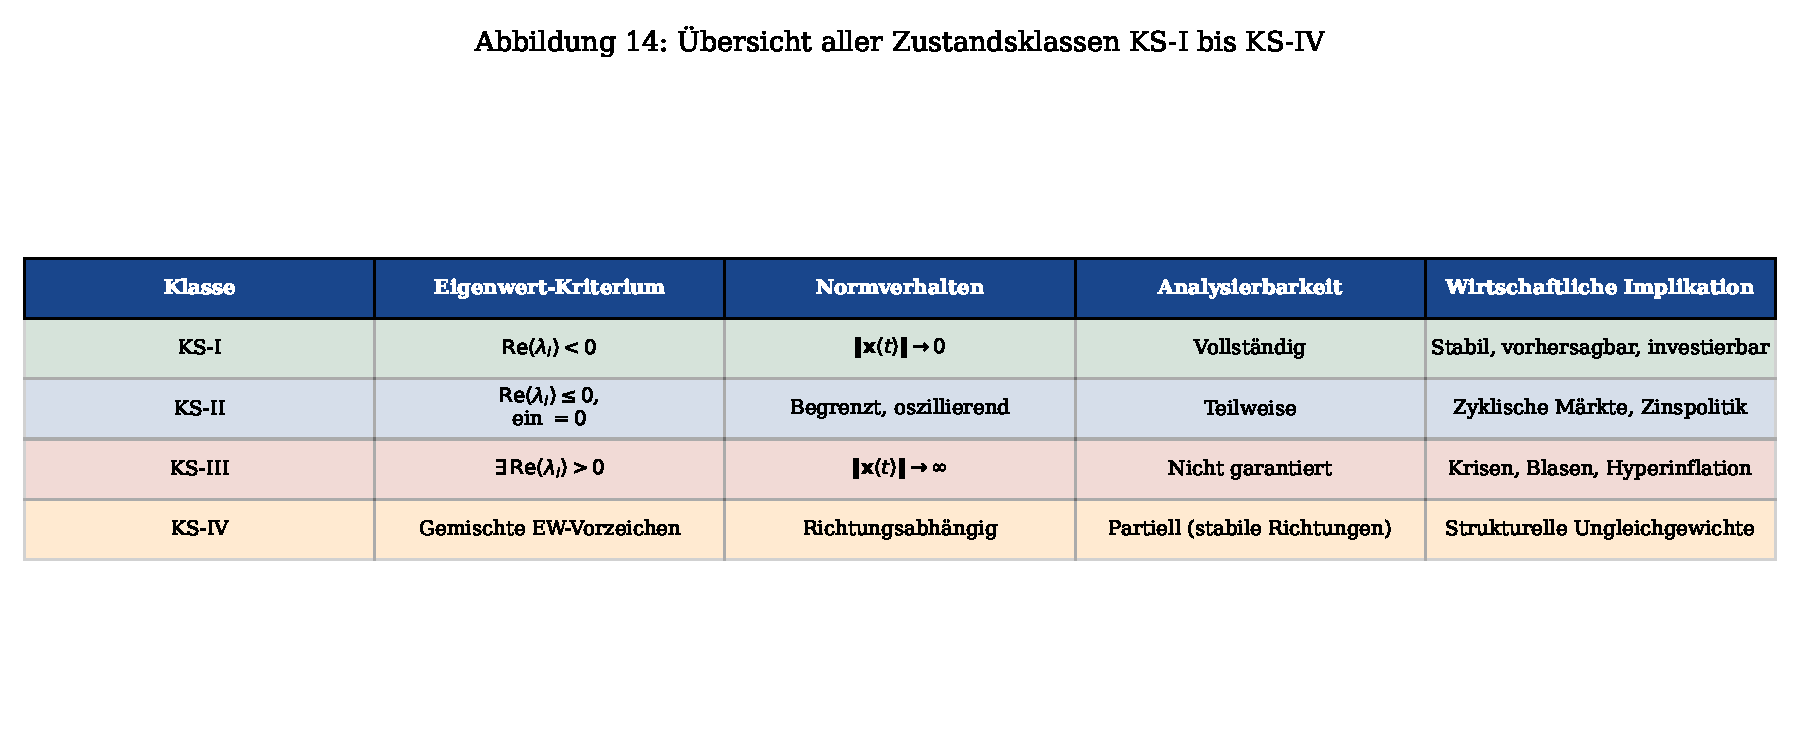
\includegraphics[width=\textwidth]{fig14_tabelle.pdf}
  \caption{Ãœbersicht aller Zustandsklassen KS-I bis KS-IV mit Eigenwertkriterium,
    Normverhalten, Analysierbarkeit und wirtschaftlicher Implikation.}
  \label{fig:tabelle}
\end{sidewaysfigure}

Die vorliegende Arbeit hat ausgehend von der fundamentalen Frage der
\emph{Endlichkeit des Zustandsvektors} ein vollständiges, formal bewiesenes Framework
für die Klassifikation dynamischer Systeme und deren wirtschaftliche Interpretation
entwickelt. Die zentralen Ergebnisse sind:

\begin{enumerate}[label=(\roman*)]
  \item \textbf{Endlichkeit als Fundamentalbedingung:} Die Endlichkeit
    $\sup_{t\geq 0}\|\vx(t)\|_2 < \infty$ ist die notwendige Voraussetzung für
    jede Stabilitäts- und Güteanalyse. Systeme ohne diese Eigenschaft (KS-III)
    sind für alle Zeiten prinzipiell nicht garantiert analysierbar.

  \item \textbf{Vier Zustandsklassen:} KS-I (asymptotisch stabil), KS-II
    (grenzstabil, oszillierend), KS-III (instabil, divergent) und KS-IV
    (hyperbolisch, richtungsabhängig) decken alle möglichen Systemkonfigurationen
    vollständig und disjunkt ab.

  \item \textbf{Subgraph Algorithmus:} Der Subgraph Algorithmus~\citep{epp2026subgraph}
    bestimmt in $\Theta(n^3)$ -- asymptotisch optimal unter SETH -- ob zwei
    Systemgraphen in zyklischer Subgraph-Beziehung stehen. Die injektive
    Signaturfunktion und die Beschränkung auf $n$ zyklische Rotationen reduzieren
    das superexponentielle Permutationsproblem auf kubische Komplexität.
    Die Subgraph-Relation vermittelt Stabilitätseigenschaften, Steuerbarkeit und
    ermöglicht die informationstheoretisch fundierte Deduplizierung konkurrierender
    Systemmodelle.

  \item \textbf{Graph-Systemmatrix-Korrespondenz:} Die Systemmatrix $\vA$ induziert
    einen Systemgraphen $\mathcal{G}(\vA)$, auf den die gesamte Graphentheorie
    anwendbar ist. Der Subgraph Algorithmus (SA) kombiniert Eigenwertanalyse,
    SCC-Zerlegung und Lyapunov-Synthese zu einem vollständigen Analysewerkzeug
    in $O(n^3)$.

  \item \textbf{Wirtschaft als angewandte Mathematik:} Es gibt keine eigenständige
    Finanztheorie. Jedes Wirtschaftsmodell ist ein dynamisches System, und alle
    qualitativen Aussagen über Stabilität, Zyklen, Krisen und Robustheit sind
    vollständig durch $\KS(\vA)$ bestimmt. Die Zustandsklassifikation ersetzt
    intuitive Konzepte durch mathematisch exakte Kennzahlen.

  \item \textbf{Formale Beweise:} Alle Hauptaussagen -- von der Spektralcharakterisierung
    der Endlichkeit (Theorem~\ref{thm:endlichkeit}) über die Lyapunov-Gleichung
    (Theorem~\ref{thm:ks1}) bis zur wirtschaftlichen Steuerbarkeit
    (Theorem~\ref{thm:wirtschaft_steuern}) -- wurden vollständig bewiesen.

  \item \textbf{Graphprofilverteilung:} Die Integration der Graphprofiltheorie
    aus~\citep{epp2026graphs} zeigt, dass jede Zustandsklasse ein charakteristisches
    Graphprofil $(D, L, \kappa)$ besitzt. Grenzstabile Systeme (KS-II) weisen
    mit $\kappa = 0{,}149$ das signifikant kleinste Kantenmaß und mit
    $\mathrm{diam} = 1{,}64$ den kleinsten Durchmesser auf, während KS-I und KS-III
    symmetrische Profile zeigen ($\kappa \approx 0{,}21$, $\mathrm{diam} \approx 2{,}2$).
    Der dichteabhängige Phasenübergang der Zustandsklassenverteilung eröffnet neue
    Möglichkeiten für das strukturelle Systemdesign.
\end{enumerate}

Die Zustandsklassifikation ist das fehlende Bindeglied zwischen der abstrakten linearen
Algebra der Systemmatrix und den konkreten Eigenschaften des dynamischen Systems --
in Ingenieurwesen, Physik und Wirtschaft gleichermaßen. Der Subgraph Algorithmus
macht diese Klassifikation algorithmisch effizient zugänglich und öffnet die gesamte
Graphentheorie als Werkzeugkasten für die Systemanalyse.

% ============================================================
\chapter{Ausblick}
\label{sec:ausblick}
% ============================================================

Die in dieser Arbeit entwickelten Grundlagen -- Zustandsklassen KS-I bis KS-IV,
Graph-Systemmatrix-Korrespondenz, Subgraph Algorithmus und Subgraph Algorithmus --
bilden ein geschlossenes Framework, das jedoch zugleich zahlreiche Richtungen für
weiterführende Forschung eröffnet. Der folgende Ausblick gliedert diese
Forschungsperspektiven systematisch in neun thematische Schwerpunkte. Dabei wird
zwischen kurzfristig erreichbaren Erweiterungen, mittelfristigen Forschungsprogrammen
und langfristigen theoretischen Grundlagenfragen unterschieden.

% ------------------------------------------------------------
\section{Zeitvariante und Periodische Systeme}
\label{subsec:zeitvariant}
% ------------------------------------------------------------

Die vorliegende Arbeit beschränkt sich bewusst auf \emph{lineare zeitinvariante} (LTI)
Systeme, da diese die sauberste algebraische Theorie besitzen: Eigenwerte, Spektrum und
Matrixexponential sind zeitunabhängige Objekte, und die Zustandsklassen KS-I bis KS-IV
sind im eigentlichen Sinne statische Typzuweisungen. Die natürliche erste
Verallgemeinerungsstufe sind \emph{lineare zeitvariante} (LTV) Systeme
\begin{equation}
  \dot{\vx}(t) = \vA(t)\vx(t), \quad \vA : [0,\infty) \to \R^{n \times n}.
  \label{eq:ltv}
\end{equation}
Für LTV-Systeme versagt das algebraische Eigenwertkriterium fundamental: Es gibt
Matrizen $\vA(t)$ mit $\re(\lambda_k(\vA(t))) < 0$ für alle $t \geq 0$ und trotzdem
divergierenden Trajektorien (klassisches Beispiel von Bellman 1953). Die richtige
Verallgemeinerung der Spektralabszisse sind die \emph{Lyapunov-Exponenten}:
\begin{equation}
  \chi_k := \limsup_{t \to \infty} \frac{1}{t} \log \| \Phi(t,0)\bm{v}_k \|,
  \label{eq:lyapunov_exp}
\end{equation}
wobei $\Phi(t,0)$ das Fundamentalsystem von~\eqref{eq:ltv} bezeichnet und $\bm{v}_k$
geeignet gewählte Anfangsvektoren sind. Eine \emph{erweiterte Zustandsklassifikation
für LTV-Systeme} würde die Bedingungen aus Definition~\ref{def:klassen} durch
Vorzeichen der Lyapunov-Exponenten $\chi_k$ ersetzen:
\begin{alignat}{2}
  \KS\text{-I}_\chi  &:\quad &\max_k \chi_k &< 0 \quad (\text{uniform exp. stabil})\\
  \KS\text{-II}_\chi &:\quad &\max_k \chi_k &= 0 \quad (\text{kritisch})\\
  \KS\text{-III}_\chi&:\quad &\max_k \chi_k &> 0 \quad (\text{instabil})
\end{alignat}
Die numerische Berechnung der Lyapunov-Exponenten ist ein aktives Forschungsfeld;
der QR-Algorithmus von Benettin et al.~(1980) liefert praktisch einsetzbare Schätzungen,
ist jedoch rechenzeitkritisch für hochdimensionale Wirtschaftsmodelle.

Für \emph{periodische Systeme} $\vA(t+T) = \vA(t)$ bietet die Floquet-Theorie
eine exakte Brücke: Jedes $T$-periodische System ist (global) äquivalent zu einem
LTI-System mit Systemmatrix $\vA_F := \frac{1}{T}\log \Phi(T,0)$ (\emph{Floquet-Matrix}).
Die Zustandsklasse des Floquet-Systems ist damit wieder durch Eigenwerte von $\vA_F$
definiert -- dies schließt die Konjunkturzyklusmodelle (Theorem~\ref{thm:zyklen}) direkt
ein und erweitert sie auf nicht autonome periodische Störungen (saisonale Wirtschaftszyklen,
geldpolitische Intervall\-entscheidungen).

\begin{remark}[Forschungsdesiderat: Automatische Floquet-Analyse]
Eine algorithmische Pipeline, die aus beobachteten Wirtschaftszeitreihen automatisch
eine Floquet-Matrix $\vA_F$ identifiziert und sodann die Zustandsklasse $\KS(\vA_F)$
bestimmt, würde die strukturelle Basis für eine quantitative Konjunkturprognose
liefern, die vollständig auf der Systemtheorie des Kapitels~\ref{sec:klassen}
beruht.
\end{remark}

% ------------------------------------------------------------
\section{Stochastische Erweiterungen: Itô-Stabilität und Zustandsklassen}
\label{subsec:stochastisch}
% ------------------------------------------------------------

Wirtschaftliche Systeme sind inhärent stochastisch: Nachfrageschocks,
Technologieinnovationen, politische Ereignisse und Wetterphänomene erzeugen
kontinuierliche Zustandsrauschterme, die in deterministischen LTI-Modellen nicht
modellierbar sind. Die kanonische stochastische Erweiterung ist das lineare
Itô-Differentialgleichungssystem:
\begin{equation}
  \mathrm{d}\vx(t) = \vA\vx(t)\,\mathrm{d}t + \sum_{k=1}^m \vSigma_k\vx(t)\,\mathrm{d}W_k(t),
  \label{eq:ito_system}
\end{equation}
wobei $W_k(t)$ unabhängige Standard-Wienerprozesse und $\vSigma_k \in \R^{n \times n}$
Diffusionsmatrizen sind. Für dieses System muss das Stabilitätskriterium fundamental
überarbeitet werden: Die Itô-Formel liefert für $V(\vx) = \|\vx\|^2$:
\begin{equation}
  \mathrm{d}V = \Bigl(2\vx^\T\vA\vx + \sum_k \|\vSigma_k\vx\|^2\Bigr)\mathrm{d}t
    + 2\sum_k \vx^\T\vSigma_k\vx\,\mathrm{d}W_k,
  \label{eq:ito_formel}
\end{equation}
und die stochastische Stabilität hängt nicht mehr allein von $\vA$, sondern vom
\emph{kombinierten Stabilitätsoperator}
\begin{equation}
  \mathcal{L}V(\vx) = 2\vx^\T\vA\vx + \sum_k \vx^\T\vSigma_k^\T\vSigma_k\vx
  = \vx^\T\!\left(2\vA + \sum_k \vSigma_k^\T\vSigma_k\right)\!\vx
  \label{eq:stabop}
\end{equation}
ab. Die stochastische Zustandsklassifikation wäre folglich durch die Eigenwerte der
\emph{stochastischen Systemmatrix}
\begin{equation}
  \tilde{\vA} := \vA + \tfrac{1}{2}\sum_k \vSigma_k^\T\vSigma_k
  \label{eq:stoch_sysmat}
\end{equation}
definiert. Man beachte, dass das Rauschen die effektive Systemmatrix verschiebt: Ein
deterministisch grenzstabiles KS-II-System kann durch multiplicatives Rauschen
entweder stabilisiert oder destabilisiert werden -- ein Phänomen, das als
\emph{stochastische Resonanz} bzw.~\emph{Noise-induced instability} bekannt ist und
in wirtschaftlichen Modellen bei Zinsdynamiken beobachtbar ist (CIR-Modell, Vasicek-Modell).

\begin{proposition}[Stochastische Zustandsklassen, vorläufig]
Für das Itô-System~\eqref{eq:ito_system} mit stochastischer Systemmatrix $\tilde{\vA}$
gemäß~\eqref{eq:stoch_sysmat} gelten die Zustandsklassen KS-I bis KS-IV aus
Definition~\ref{def:klassen} mit $\vA$ ersetzt durch $\tilde{\vA}$ für die
mittlere quadratische Stabilität (mean-square stability). Die Berechnung von
$\KS(\tilde{\vA})$ verläuft algorithmisch identisch durch den Subgraph Algorithmus.
\end{proposition}

\noindent
Die vollständige Ausarbeitung dieser Verallgemeinerung -- insbesondere der Nachweis
der Äquivalenz stochastischer Lyapunov-Bedingungen mit den Eigenwertkriterien für
$\tilde{\vA}$ -- stellt ein eigenständiges Forschungsprogramm dar.

% ------------------------------------------------------------
\section{Nichtlineare Systeme: Globale Klassifikation und Bifurkationstheorie}
\label{subsec:nichtlinear}
% ------------------------------------------------------------

Abschnitt~\ref{sec:konsequenzen} hat angemerkt, dass die Jacobi-Matrix $\vA^*$ am
Gleichgewicht $\vx^*$ die \emph{lokale} Zustandsklasse eines nichtlinearen Systems
bestimmt (Satz von Hartman-Grobman). Diese lokale Sichtweise ist für viele wirtschaftliche
Fragestellungen unzureichend, da Märkte und Volkswirtschaften typischerweise
\emph{multiple Gleichgewichte} besitzen: stationäre Punkte, Grenzzyklen, Attraktoren und
chaotische Mengen koexistieren im gleichen Zustandsraum.

Eine weiterführende Forschungsfrage ist:

\begin{enumerate}[label=\textbf{A\arabic*.}]
  \item \textbf{Globale KS-Karte:} Für ein nichtlineares System $\dot{\vx} = f(\vx)$
    mit mehreren Gleichgewichten $\vx_1^*, \ldots, \vx_r^*$ definiert jede
    Jacobi-Matrix $\vA_i^* = \partial f/\partial\vx|_{\vx_i^*}$ eine lokale
    Zustandsklasse $\KS(\vA_i^*)$. Die \emph{globale KS-Karte} des Systems wäre
    die Abbildung $\vx \mapsto \KS(\vA^*(\vx))$, sofern $\vx$ im Einzugsgebiet
    eines Gleichgewichts liegt. Diese Karte partitioniert den Zustandsraum nach
    lokalen Stabilitätseigenschaften und hat direkte Interpretation als ``Risikokarte''
    für Wirtschaftssysteme.

  \item \textbf{Bifurkationen als Klassenwechsel:} Ein Parameterwechsel in einem
    nichtlinearen Wirtschaftsmodell (z.\,B. Erhöhung des Leitzinses) kann einen
    Eigenwert durch die imaginäre Achse bewegen und damit einen Klassenwechsel
    auslösen. Die Hopf-Bifurkation ($\vA^*$-Eigenwert überquert die imaginäre Achse
    als konjugiertes Paar) entspricht dem Ãœbergang KS-I $\to$ KS-II, die
    Sattel-Knoten-Bifurkation (reeller Eigenwert durch Null) dem Ãœbergang KS-I $\to$ KS-IV.
    Eine systematische Bifurkationsanalyse im Rahmen der Zustandsklassen würde eine
    quantitative Theorie wirtschaftlicher Phasenübergänge liefern.

  \item \textbf{Barrier-Funktionen als globale Lyapunov-Ersatz:} Für globale
    Stabilitätsaussagen nichtlinearer Systeme bieten Barrier-Zertifikatsmethoden
    (Prajna \& Jadbabaie, 2004) eine Alternative zu lokalen Lyapunov-Funktionen.
    Die Verbindung zu den Zustandsklassen über Sum-of-Squares-(SOS-)Optimierung
    ermöglicht die automatische Synthese globaler Stabilitätszertifikate.
\end{enumerate}

% ------------------------------------------------------------
\section{Datengetriebene Identifikation der Zustandsklasse}
\label{subsec:datengetrieben}
% ------------------------------------------------------------

In der wirtschaftlichen Praxis ist die Systemmatrix $\vA$ selten direkt bekannt.
Stattdessen liegen Zeitreihendaten $\vx(t_0), \vx(t_1), \ldots, \vx(t_N)$ vor,
aus denen sowohl $\vA$ als auch $\KS(\vA)$ inferiert werden müssen. Dies führt zum
\emph{System-Identifikationsproblem der Zustandsklassen}, das wir als
eigenständiges Forschungsfeld skizzieren:

\subsubsection*{Koopman-Operator-Methoden}

Der \emph{Koopman-Operator} $\mathcal{K}$ eines nichtlinearen Systems
$\dot{\vx} = f(\vx)$ ist der lineare Operator auf dem Raum der Observablen
$g : \R^n \to \R$:
\begin{equation}
  (\mathcal{K} g)(\vx) = \nabla g(\vx) \cdot f(\vx).
  \label{eq:koopman}
\end{equation}
Obwohl $f$ nichtlinear ist, ist $\mathcal{K}$ linear -- allerdings auf einem
unendlichdimensionalen Funktionenraum. Moderne Methoden wie die \emph{Dynamic Mode
Decomposition} (DMD) und ihre Erweiterungen (EDMD, DMDc) approximieren $\mathcal{K}$
durch eine endlichdimensionale Koopman-Matrix $\hat{\vK} \in \R^{p \times p}$
aus Daten. Die Eigenwerte von $\hat{\vK}$ (die \emph{Koopman-Eigenwerte}) konvergieren
unter geeigneten Annahmen gegen die Eigenwerte von $\mathcal{K}$, und ihr Spektrum
enthält die dynamische Information des ursprünglichen Systems.

\begin{remark}[Zustandsklassen via Koopman-Eigenwerte]
Die Zustandsklasse $\KS(f)$ eines nichtlinearen Systems $\dot{\vx} = f(\vx)$ im globalen
Sinne könnte durch das Spektrum des Koopman-Operators $\mathcal{K}$ definiert werden:
Liegen alle Koopman-Eigenwerte mit negativem Realteil, so entspricht dies einem
KS-I-Verhalten im Koopman-Bild. Diese Verallgemeinerung harmoniert mit der
bekannten Tatsache, dass für LTI-Systeme Koopman-Eigenwerte und Systemmatrix-Eigenwerte
identisch sind.
\end{remark}

\subsubsection*{Sparse Identification of Nonlinear Dynamics (SINDy)}

Das SINDy-Verfahren (Brunton et al., 2016) identifiziert aus Zeitreihendaten die
spärlichste Darstellung $\dot{\vx} \approx \bm{\Theta}(\vx)\bm{\Xi}$, wobei
$\bm{\Theta}$ eine Bibliothek von Basisfunktionen und $\bm{\Xi}$ eine Koeffizientenmatrix
ist. Für lineare Systeme ergibt SINDy direkt die Systemmatrix $\vA = \bm{\Xi}^\T$,
und damit $\KS(\vA)$ durch direkten Eigenwertvergleich. Für nichtlineare Systeme
liefert SINDy eine Approximation $f \approx \hat{f}$, deren Linearisierung als
Näherung für $\KS$ dienen kann.

\subsubsection*{Maschinelles Lernen und spektrale Klassifikatoren}

Eine dritte, rein datengetriebene Richtung ist das Training von Klassifikatoren
(neuronale Netze, Support-Vector-Machines, Random Forests), die direkt aus
Zeitreiheneigenschaften (Autokorrelationsfunktionen, Hurst-Exponenten,
Leistungsspektren) auf die Zustandsklasse $\KS$ schließen. Erste Ergebnisse aus
der Nichtlineare-Dynamik-Literatur zeigen, dass solche Klassifikatoren hohe
Genauigkeit erreichen, sobald geeignete spektrale Merkmale als Features gewählt werden.
Die formale Brücke zwischen diesen empirischen Klassifikatoren und den mathematisch
exakten Definitionen aus Abschnitt~\ref{sec:klassen} steht noch aus.

% ------------------------------------------------------------
\section{Netzwerke Gekoppelter Systeme und Multilevel-Subgraph}
\label{subsec:netzwerke}
% ------------------------------------------------------------

Makroökonomische Systeme bestehen nicht aus einer einzelnen Volkswirtschaft, sondern
	aus einem \emph{Netzwerk} von Volkswirtschaften, die über Handelsströme, Kapitalflüsse
und Währungskopper\-bindungen interagieren. Formal ist ein solches System beschreibbar
als \emph{gekoppeltes LTI-Netz}:
\begin{equation}
  \dot{\vx}_i(t) = \vA_i\vx_i(t) + \sum_{j=1}^{N} \vC_{ij}\vx_j(t), \quad i = 1, \ldots, N,
  \label{eq:netz}
\end{equation}
wobei $\vA_i \in \R^{n_i \times n_i}$ die Systemmatrix der $i$-ten Volkswirtschaft,
$\vC_{ij} \in \R^{n_i \times n_j}$ die Kopplungsmatrix von $j$ nach $i$
und $N$ die Anzahl der Volkswirtschaften bezeichnen. Das Gesamtsystem hat die
Block-Systemmatrix
\begin{equation}
  \vA_{\mathrm{net}} = \begin{pmatrix}
    \vA_1 & \vC_{12} & \cdots & \vC_{1N} \\
    \vC_{21} & \vA_2 & \cdots & \vC_{2N} \\
    \vdots & & \ddots & \vdots \\
    \vC_{N1} & \vC_{N2} & \cdots & \vA_N
  \end{pmatrix}.
  \label{eq:blockmat}
\end{equation}

\begin{remark}[Zustandsklasse des Gesamtnetzwerks versus Teilsystemen]
Aus Proposition~\ref{prop:scc_stab} folgt, dass das Gesamtnetzwerk nur dann KS-I ist,
wenn alle Diagonalblöcke $\vA_i$ zu KS-I gehören \emph{und} die Kopplungen $\vC_{ij}$
die Gesamtstabilität nicht zerstören. Die präzise Bedingung auf $\vC_{ij}$ führt auf
das Problem der \emph{kompositionellen Stabilität}, das in der Regelungstheorie als
``small-gain theorem'' bekannt ist. Im wirtschaftlichen Kontext fragt dieses Kriterium:
Unter welchen Handelsbedingungen bleibt ein Netzwerk aus KS-I-Volkswirtschaften global stabil?
\end{remark}

\subsubsection*{Multilevel-Subgraph Algorithmus}

Für Systeme der Form~\eqref{eq:netz} bietet der Subgraph Algorithmus eine natürliche
\emph{hierarchische Erweiterung}: Der \emph{Multilevel-Subgraph} $\mathcal{S}_{\mathrm{net}}$
besteht aus
\begin{itemize}
  \item einem \emph{Metagraphen} auf Ebene 2, dessen Knoten die Volkswirtschaften
    $1, \ldots, N$ und dessen Kanten die nichtver\-schwindenden Kopplungsblöcke
    $\vC_{ij} \neq \bm{0}$ sind,
  \item je einem Subgraph $\mathcal{S}(\vA_i)$ als Knoten-Annotation auf Ebene 1.
\end{itemize}
Die SCC-Zerlegung des Metagraphen (Kosaraju auf Ebene 2) identifiziert
\emph{Systemcluster}: Volkswirtschaften, die zyklisch voneinander abhängen. Der
Subgraph Algorithmus auf Ebene 1 liefert für jede Volkswirtschaft die Zustandsklasse.
Die Kombination beider Informationen erlaubt Aussagen wie: ``Cluster $\mathcal{C}$
bestehend aus KS-I- und KS-II-Volkswirtschaften hat durch seine interne Kopplungsstruktur
($\vC_{ij}$ zu groß) eine instabile Rückkopplungsschleife -- Gesamtsystem ist KS-IV.''

Die algorithmische Komplexität des Multilevel-Subgraph Algorithmus beläuft sich auf
$O(N^2 n^3)$ für den Vollvergleich aller Kopplungen, wobei $n = \max_i n_i$.
Für spärlich vernetzte Systeme (Anzahl nichtversch window Kopplungsblöcke $\ll N^2$)
verbessert sich dies auf $O(|\mathcal{E}| \cdot n^3)$, wobei $|\mathcal{E}|$ die
Anzahl der Kanten im Metagraphen bezeichnet.

% ------------------------------------------------------------
\section{Optimale Zustandsklassenübergänge und Polplatzierung}
\label{subsec:polplatz}
% ------------------------------------------------------------

Aus dem Blickwinkel der Regelungstheorie ist die natürlichste wirtschaftspolitische
Fragestellung nicht die Analyse des bestehenden Systems, sondern die
\emph{Synthese}: Wie muss eine wirtschaftspolitische Steuerung $\vu(t)$ gewählt
werden, um ein KS-III-System (Krise) in ein KS-I-System (Stabilität)
zu überführen?

\subsubsection*{Polvorgabe und Spektralformung}

Das \emph{Polvorgabeproblem} (pole placement) fragt: Gesucht ist ein linearer
Regler $\vu(t) = -\vK\vx(t)$ (Zustandsrückführung), der die Systemmatrix des
geschlossenen Regelkreises $\vA_{\mathrm{cl}} = \vA - \vB\vK$ so gestaltet, dass
$\KS(\vA_{\mathrm{cl}}) = \KS\text{-I}$ gilt. Ist das System $(\vA, \vB)$ steuerbar
(Theorem~\ref{thm:wirtschaft_steuern}), so ist dieses Problem \emph{immer} lösbar
(Ackermann-Formel, allgemeiner: Bass-Gura-Methode). Der optimale Regler -- der
$\vK$ unter minimaler Regelenergie $\int_0^\infty \vu^\T\vu\,\mathrm{d}t$ bestimmt --
ist der \emph{Linear-Quadratic Regulator} (LQR), der die algebraische Riccati-Gleichung
\begin{equation}
  \vA^\T\vP + \vP\vA - \vP\vB\vR^{-1}\vB^\T\vP + \vQ = \bm{0}
  \label{eq:riccati}
\end{equation}
löst, mit $\vK^* = \vR^{-1}\vB^\T\vP$ und positiv definiten Gewichtsmatrizen
$\vQ, \vR$. Das Wirtschaftsinterpretation von~\eqref{eq:riccati}: $\vQ$ gewichtet
die ``Kosten'' von Zustandsabweichungen (BIP-Lücke, Inflationsabweichung),
$\vR$ die Kosten wirtschaftspolitischer Eingriffe (Zinssenkungskosten,
fiskalische Schuldenaufnahme).

\subsubsection*{Minimale Perturbation für KS-III $\to$ KS-I}

Eine verwandte, fundamental neue Fragestellung: Gegeben $\vA \in \KS\text{-III}$,
gesucht ist die \emph{kleinste Perturbation} $\Delta\vA$ (im Sinne der Spektralnorm),
so dass $\vA + \Delta\vA \in \KS\text{-I}$:
\begin{equation}
  \min_{\Delta\vA} \|\Delta\vA\|_2 \quad \text{s.\,d.} \quad
  \max_k \re(\lambda_k(\vA + \Delta\vA)) < 0.
  \label{eq:minpert}
\end{equation}
Das Problem~\eqref{eq:minpert} ist das strukturelle Gegenstück zur
Stabilitätsoptimierung. Seine Lösung -- die \emph{Distanz zum instabilen Rand} (distance
to instability) -- verallgemeinert den Stabilitätsabstand $\delta$ aus
Proposition~\ref{prop:robustheit} und misst, wie viel Strukturveränderung benötigt wird,
um ein Krisensystem zu stabilisieren. In wirtschaftspolitischer Sprache: Welches ist
der kleinstmögli\-che System\-eingriff (Zinsänderung, Regulierung, fiskalisches Paket),
der das System von KS-III nach KS-I transferiert?

Algorithmen zur Berechnung dieser Distanz (Guglielmi, Gürbüzbalaban, Overton, 2017)
haben Komplexität $O(n^3)$ pro Iteration und sind für Wirtschaftssystemmatrizen
bis $n \approx 500$ praktisch einsetzbar.

\subsubsection*{$\mathcal{H}_\infty$-Synthese als robuste Klassensicherung}

Ãœber den LQR hinaus liefert die $\mathcal{H}_\infty$-Synthese einen Regler, der
die KS-I-Klassenzugehörig\-keit auch unter Modellunsicherheiten $\|\Delta\vA\|_2 < \varepsilon$
aufrecht\-erhält (robuste Stabilität). Die zugehörige $\mathcal{H}_\infty$-Norm
\[
  \|(\vI + \vG\vK)^{-1}\vG\|_\infty
\]
quantifiziert, wie stark externe Störungen
(wirtschaftliche Schocks) die Zustandsnorm beeinflussen. Systeme mit kleiner
$\mathcal{H}_\infty$-Norm sind durch Proposition~\ref{prop:robustheit} ``tief''
in der KS-I-Klasse verankert.

% ------------------------------------------------------------
\section{Erweiterungen des Subgraph Algorithmus}
\label{subsec:subgraph_erw}
% ------------------------------------------------------------

Der in Kapitel~\ref{sec:subgraph} vollständig analysierte Subgraph Algorithmus
\citep{epp2026subgraph} ist in seiner aktuellen Form auf quadratische
$n \times n$-Adjazenzmatrizen und zyklische Rotationen beschränkt. Mehrere
Erweiterungsrichtungen sind von unmittelbarem theoretischem und praktischem Interesse:

\subsubsection*{Gewichtete Systemgraphen}

In realen Wirtschaftssystemen tragen die Kanten von $\mathcal{G}(\vA)$ Gewichte
(die Matrixeinträge $a_{ij} \in \R$), nicht nur Binärinformation. Die aktuelle
Signaturfunktion~\eqref{eq:signatur} ignoriert diese Gewichte. Eine gewichtete
Signatur könnte durch
\begin{equation}
  \sigma_j^w(A) := \sum_{i=0}^{n-1} \lfloor A_{ij} \cdot 2^b \rfloor \cdot p_i + j \cdot P_n
  \label{eq:weight_sig}
\end{equation}
definiert werden, wobei $b$ die Quantisierungsgenauigkeit, $p_i$ paarweise teilerfremde
Primzahlen (Chinese Remainder Theorem) und $P_n = \prod_{i=0}^{n-1} p_i$ bezeichnen.
Die Injektivität dieser gewichteten Signatur wäre unter geeigneten Ganzzahl-
Quantisierungsannahmen beweisbar, und die Komplexität bliebe $O(n^3)$ mit einem
Faktor $O(b)$ für die Ganzzahlarithmetik.

\subsubsection*{Nicht-quadratische und heterogene Systeme}

Für Netzwerke aus Systemen verschiedener Dimension ($n_1 \neq n_2$) müssen die
Adjazenzmatrizen $A \in \{0,1\}^{n_1 \times n_1}$ und $B \in \{0,1\}^{n_2 \times n_2}$
verglichen werden. Das \emph{induced subgraph isomorphism problem} fragt ob
$\mathcal{G}(\vB)$ einen Teilgraphen enthält, der isomorph zu $\mathcal{G}(\vA)$ ist --
ein NP-vollständiges Problem im Allgemeinen. Für die systemtheoretisch relevante
zyklische Subgraph-Relation könnte die Beschränkung auf zyklustreue Einbettungen
(d.\,h. Einbettungen, die Zyklen auf Zyklen abbilden) wieder eine polynomielle
Entscheidbarkeit ergeben. Dies ist eine offene Frage.

\subsubsection*{Dynamischer Subgraph-Vergleich}

In zeitvarianten Kontexten variiert die Systemmatrix $\vA(t)$, und damit auch
der Systemgraph $\mathcal{G}(\vA(t))$. Ein \emph{dynamischer Subgraph-Vergleich}
würde für zwei zeitvariante Systeme $\vA(t)$ und $\vB(t)$ fragen, ob die
Subgraph-Relation $\mathcal{G}(\vA(t)) \subseteq \mathcal{G}(\vB(t))$ für alle
$t \in [0, T]$ gilt. Dies ist äquivalent zur Frage, ob die \emph{Unterstützung}
(support) von $\vA(t)$ stets in der Unterstützung von $\vB(t)$ enthalten ist --
eine Eigenschaft, die prüfbar ist, wenn Strukturwechselzeitpunkte bekannt sind.

\subsubsection*{Parallelisierung und verteilte Berechnung}

Für sehr große Systemmatrizen ($n > 10^4$, wie sie etwa bei Eingabe-Output-Analysen
von Volkswirtschaften mit mehreren tausend Sektoren auftreten) ist die sequentielle
$\Theta(n^3)$-Laufzeit des Subgraph Algorithmus zu langsam. Da die $n$ LCS-Berechnungen
für verschiedene Rotationen vollständig unabhängig sind (Beweis zu
Theorem~\ref{thm:optimalitaet_subgraph}), ist der Algorithmus trivial parallelisierbar:
Auf einem $p$-Prozessor-System ergibt sich eine parallele Laufzeit von
$O(n^3/p + n^2)$, was für $p = O(n)$ Prozessoren eine Laufzeit $O(n^2)$ ergibt.
Moderne GPU-Implementierungen erlauben in der Praxis $p \sim 10^4$, was
Systemmatrizen der Dimension $n \sim 5000$ in Millisekunden analysierbar macht.

% ------------------------------------------------------------
\section{Verbindungen zu anderen Mathematischen Disziplinen}
\label{subsec:math_verbindungen}
% ------------------------------------------------------------

Die in dieser Arbeit entwickelten Konzepte berühren mehrere tiefe mathematische
Forschungsfelder, die bislang noch keine systematische Verbindung zur Zustandsklassifikation
hatten.

\subsubsection*{Algebraische Topologie: Persistente Homologie des Systemgraphen}

Die \emph{persistente Homologie} (Carlsson, 2009) extrahiert topologische
Invarianten (Betti-Zahlen, Barcode) aus gefilterten Simplizialkomplexen. Angewendet
auf den Systemgraphen $\mathcal{G}(\vA)$ -- gefiltert nach dem Absolutwert der
Kantengewichte $|a_{ij}|$ -- liefert die persistente Homologie eine
topologische Signatur des dynamischen Systems. Interessant ist die Frage: Korrelieren
diese topologischen Signaturen mit der Zustandsklasse? Erste heuristische Befunde
aus der Netzwerkwissenschaft deuten darauf hin, dass KS-I-Systeme charakteristisch
einfachere Barcodes aufweisen als instabile Systeme.

\subsubsection*{Spektralgeometrie und Laplace-Spektrum}

Der \emph{Laplace-Operator} $L = D - A$ eines Graphen (mit Gradmatrix $D$ und
Adjazenzmatrix $A$) hat engen Bezug zur Systemmatrix $\vA$: Für symmetrische $\vA$
mit Zeilensumme Null stimmt $-\vA$ mit dem Laplace-Operator überein. Die Eigenwerte
des Laplacians (Laplace-Spektrum) steuern Diffusions- und Synchronisationsprozesse
auf Graphen. Die bereits bekannte Fiedler-Zahl $\lambda_2(L)$ (smallest nontrivial
eigenvalue) quantifiziert die algebraische Konnektivität und damit die
Resilienz des gekoppelten Netzwerks -- eine direkte Verbindung zur Robustheit
aus Proposition~\ref{prop:robustheit}.

\subsubsection*{Kategorientheorie: Funktorialität der Zustandsklassenabbildung}

Aus einem hohen Abstraktionsniveau betrachtet ist die Abbildung
$\vA \mapsto \KS(\vA)$ ein Funktor von der Kategorie der reellen Matrizen
(mit Konjugation als Morphismus) in eine Kategorie mit vier Objekten
$\{\KS\text{-I}, \KS\text{-II}, \KS\text{-III}, \KS\text{-IV}\}$.
Die Natürlichkeit dieser Abbildung -- d.\,h. die Frage, ob strukturerhaltende
Transformationen (Ähnlichkeitstransformationen $\vA \mapsto \vS\vA\vS^{-1}$)
die Klasse erhalten -- ist trivialerweise erfüllt, da Eigenwerte unter
Ähnlichkeitstransformation invariant sind. Interessanter sind \emph{strukturelle
Morphismen}, etwa Netzwerkhomomorphismen $\mathcal{G}(\vA) \to \mathcal{G}(\vB)$:
Welche Eigenschaften der Zustandsklassen werden durch solche Morphismen bewahrt?

\subsubsection*{Informationstheorie: Maximale Entropie und Systemklassen}

Das \emph{Maximum-Entropie-Prinzip} (Jaynes, 1957) fragt nach der
wahrscheinlichsten Systemmatrix $\vA$ unter gegebenen Informationseinschränkungen.
Für die Einschränkung $\alpha^* = \alpha_0$ (feste Spektralabszisse) ist die
Verteilung über Systemmatrizen durch ein Gibbs-Maß mit dem Exponenten $\alpha^*$
als ``inverse Temperatur'' charakterisiert. Die Zustandsklassen entsprechen in
diesem Bild thermodynamischen Phasen, und die Übergänge KS-I $\leftrightarrow$ KS-II
etc.\ sind Phasenübergänge. Diese Analogie hat Konsequenzen für die statistische
Schätzung von Systemmatrizen aus Daten: Die Maximum-Entropie-Schätzung unter der
Nebenbedingung $\KS(\hat{\vA}) = \KS\text{-I}$ liefert einen strukturell stabilen
Schätzer.

% ------------------------------------------------------------
\section{Wirtschaftspolitische Implikationen: Regulierung und Systemdesign}
\label{subsec:wirtschaftspolitik}
% ------------------------------------------------------------

Die Kernthese dieser Arbeit -- dass Wirtschaftssysteme vollständig durch
ihre Systemmatrix charakterisierbar sind -- hat weitreichende Konsequenzen für
Wirtschaftspolitik, Finanzregulierung und institutionelles Design.

\subsubsection*{Zustandsklassenbasierte Regulierungsarchitektur}

Eine auf den Zustandsklassen basierende Regulierungsarchitektur würde Folgendes umfassen:

\begin{enumerate}[label=\textbf{R\arabic*.}]
  \item \textbf{Pflichtklassifikation systemrelevanter Institute:}
    Jede systemrelevante Bank, jeder Versicherungskonzern und jeder Staatsfonds
    müsste vierteljährlich die Zustandsklasse seines internen Dynamikmodells
    $\KS(\vA_{\mathrm{inst}})$ an die Regulierungsbehörde melden. Dies wäre der
    mathematisch präzise und nicht manipulierbare Ersatz für aktuelle
    qualitative Stressszenarien (DFAST, EBA-Stresstests).

  \item \textbf{Systemischer Risikopuffer als Funktion von $\delta$:}
    Der Stabilitätsabstand $\delta = -\alpha^*(\vA_{\mathrm{inst}})$ liefert
    eine natürliche, quantitative Grundlage für Kapitalpuffer-Anfor\-derungen:
    Je kleiner $\delta$, desto näher das System am instabilen Rand, desto
    höher der geforderte Kapitalpuffer. Eine Regulierungs\-formel der Form
    $\mathrm{Puffer}(t) \propto \exp(-c \cdot \delta(t))$ hätte automatische
    antizyklische Eigenschaften.

  \item \textbf{Netzwerkregulierung mittels Multilevel-Subgraph:}
    Der Multilevel-Subgraph Algorithmus (Kapitel~\ref{subsec:netzwerke}) erlaubt
    die Bestimmung, welche Kopplung $\vC_{ij}$ (Interbanktransaktion, Kreditlinie,
    Derivatkontrakt) das Gesamtnetzwerk am stärksten destabilisiert. Regulierung
    kann dann gezielt diese Verbindungen unter Volumen- oder Konzentrationsschranken
    setzen.

  \item \textbf{Geldpolitik als Polplatzierung:}
    Die Zinspolitik einer Zentralbank wirkt auf die Systemmatrix durch
    Änderung bestimmter Einträge (Zinselastizitäten im IS-LM-Modell, vgl.
    Beispiel~\ref{sec:wirtschaft}). Die optimale Geldpolitik ist dann formal
    identisch mit dem LQR-Problem~\eqref{eq:riccati}: Minimiere den Abstand
    zur Gleichgewichtsbahn unter minimaler Kontrollanstrengung (Zinsschwankung).
\end{enumerate}

\subsubsection*{Finanzmarktstabilität und KS-II als Zielklasse}

Eine interessante normative Frage ist, ob Volkswirtschaften überhaupt KS-I oder
vielmehr KS-II anstreben sollten. KS-I garantiert Konvergenz zum Gleichgewicht,
eliminiert aber auch wirtschaftliche Wachstumsoszillationen. KS-II mit
rein-imaginären Eigenwerten $\pm i\omega$ erzeugt nach Theorem~\ref{thm:zyklen}
persistente Zyklen -- was Innovation, schöpferische Zerstörung (Schumpeter)
und Wachstumsdynamik modellieren kann. Eine ``ideale'' Volkswirtschaft könnte
durch eine Systemmatrix $\vA^{\mathrm{ideal}}$ in KS-II mit kontrollierten
Zyklusfrequenzen $\omega$ (Konjunkturperiode $T = 2\pi/\omega \approx 7$ Jahre)
beschrieben werden. Das Regulierungsziel wäre dann nicht die Eliminierung aller
Schwingungen, sondern die Sicherstellung der Semieinfachheit der rein-imaginären
Eigenwerte -- d.\,h. die Verhinderung resonanter Verstärkung durch Jordan-Blöcke.

\subsubsection*{Digitale Zentralbankwährungen und Echtzeit-Systemklassifikation}

Digitale Zentralbankwährungen (CBDC) erzeugen Transaktionsdaten in nahezu
Echtzeit. Dies ermöglicht erstmals die kontinuierliche Schätzung der
Systemmatrix $\hat{\vA}(t)$ des monetären Sektors aus Transaktionszeitreihen
(mit Methoden aus Kapitel~\ref{subsec:datengetrieben}). Eine CBDC-Infrastruktur
könnte automatisch $\KS(\hat{\vA}(t))$ in Echtzeit überwachen und bei
Annäherung an KS-III (Auftreten von Eigen\-werten mit positivem Realteil) automatische
Gegenmaßnahmen (Liquiditäts\-injektionen, Zinssenkungen) auslösen -- ein
\emph{automatischer Stabilisator der mathematisch exakten Art}.

% ------------------------------------------------------------
\section{Implementierung, Software-Ökosystem und offene Standards}
\label{subsec:software}
% ------------------------------------------------------------

Die algorithmischen Beiträge dieser Arbeit -- Subgraph Algorithmus und
Subgraph Algorithmus -- sind auf praktische Implementierungen angewiesen,
um ihren wissenschaftlichen und wirtschaftlichen Wert voll zu entfalten.

\subsubsection*{Standardisierte Systemmatrix-Bibliothek}

Eine kuratierte, öffentlich zugängliche Bibliothek von Systemmatrizen
wirtschaftlicher Modelle (IS-LM, DSGE-Linearisierungen, Schuldendynamiken,
Portfolio-Kovarianzmatrizen) würde es erlauben, die Zustandsklassen-Klassifikation
für bekannte Modelle zu standardisieren und vergleichbar zu machen.
Analog zu den Matrix-Market-Benchmarks in der numerischen linearen Algebra
wäre eine solche Bibliothek die Grundlage für reproduzierbare Experimente.

\subsubsection*{Interoperabilität mit bestehenden Werkzeugen}

Die Zustands\-klassen\-analyse sollte nahtlos in bestehende wissenschaftliche
Software-Öko\-systeme integriert werden:
\begin{itemize}
  \item \textbf{Python/SciPy:} Erweiterung von \texttt{scipy} um
    \texttt{state\_class(A)} und \texttt{subgraph(A)},
    basierend auf der QR-Iteration von LAPACK.
  \item \textbf{Julia/ControlSystems.jl:} Einbindung der Zustandsklassenanalyse
    in das Julia-Regelungspaket durch einen neuen Systemtyp \texttt{ClassifiedLTISystem}.
  \item \textbf{MATLAB/Simulink:} Block-Bibliothek für den Subgraph Algorithmus
    mit automatischer Visualisierung des Systemgraphen und Farbkodierung
    der Zustandsklassen (analog zu \cref{fig:klassenkarte}).
  \item \textbf{R:} Paket \texttt{sysstate} für statistische Analysen von
    Systemmatrizen aus ökonometrischen Zeitreihenmodellen (VAR, VECM).
\end{itemize}

\subsubsection*{Offener Standard: KSML (Klassifikations-System-Markup-Language)}

Für den Austausch von Systemmatrizen mitsamt ihrer Zustandsklassenannotation
zwischen verschiedenen Werkzeugen und Institutionen wäre ein offener
XML/JSON-basierter Standard wünschenswert:
\begin{verbatim}
{
  "system_matrix": [[...], ...],
  "state_class": "KS-I",
  "spectral_abscissa": -0.47,
  "stability_margin": 0.47,
  "subgraph": { "scc_count": 3, "eigenvalues": [...] }
}
\end{verbatim}
Ein solcher Standard würde die Zustandsklassenanalyse zu einem reproduzierbaren,
interoperablen Werkzeug für die wissenschaftliche Gemeinschaft machen.

% ------------------------------------------------------------
\section{Zusammenfassende Forschungsagenda}
\label{subsec:agenda}
% ------------------------------------------------------------

Die folgende Tabelle fasst die gesamte Forschungsagenda in drei Zeithorizonte
zusammen:

\begin{table}[H]
\centering
\caption{Forschungsagenda: Kurzfristige, mittelfristige und langfristige Ziele}
\label{tab:agenda}
\begin{tabular}{>{\raggedright\arraybackslash}p{2.2cm}
                >{\raggedright\arraybackslash}p{5.0cm}
                >{\raggedright\arraybackslash}p{5.0cm}}
\toprule
\textbf{Horizont} & \textbf{Thema} & \textbf{Ziel} \\
\midrule
Kurzfristig & Stochastische Zustandsklassen & Beweis der mittleren quadratischen
  Äquivalenz via~$\tilde{\vA}$~\eqref{eq:stoch_sysmat} \\
 & Gewichtete Subgraph-Signatur & Injektivitätsbeweis für $\sigma_j^w$~\eqref{eq:weight_sig} \\
 & Open-Source-Implementierung & Python-Paket \texttt{sysstate} mit Subgraph + Subgraph \\
\midrule
Mittelfristig & Floquet-Analyse für Konjunktur & Automatische Pipeline: Zeitreihe $\to$
  $\vA_F \to \KS(\vA_F)$ \\
 & Multilevel-Subgraph & Algorithmus und Komplexitätsanalyse für Netzwerke~\eqref{eq:netz} \\
 & Datengetriebene KS-Klassifikation & Koopman-/SINDy-basierte Identifikation von $\KS$ \\
 & Minimale Perturbation KS-III$\to$I & Effizienter Algorithmus für~\eqref{eq:minpert} \\
\midrule
Langfristig & Globale KS-Karte & Nichtlineare Dynamik: Partitionierung des
  Zustandsraums nach lokalen KS \\
 & Topologische Invarianten & Persistente Homologie des Systemgraphen vs.\ KS \\
 & CBDC-Echtzeit-Monitor & Kontinuierliche $\hat{\vA}(t)$-Schätzung und KS-Überwachung \\
 & Regulierungsstandard & Integration in DFAST/EBA durch $\delta$-basierten Puffer \\
\bottomrule
\end{tabular}
\end{table}

Die Zustandsklassen KS-I bis KS-IV, der Subgraph Algorithmus und der Subgraph Algorithmus
sind keine Endpunkte, sondern \emph{Ausgangspunkte} einer umfassenden mathematischen
Theorie dynamischer Systeme in Ingenieurwesen, Wirtschaft und Naturwissenschaften.
Die nächste Entwicklungsstufe liegt in der Verschmelzung dieser algebraischen Theorie
mit stochastischer Analysis, datengetriebenen Methoden, Netzwerktheorie und moderner
Computational Science -- mit dem Ziel, die mathematisch exakte Systemklassifikation
zu einem universell einsetzbaren Werkzeug für Analyse, Regulierung und
wirtschaftspolitisches Design zu machen.

% ============================================================
\bibliographystyle{plainnat}
\begin{thebibliography}{99}

\bibitem[Epp(2026a)]{epp2026subgraph}
Epp, S. (2026).
\newblock \textit{Der Subgraph Algorithmus}. Verfügbar unter \url{https://github.com/hjstephan86/subgraph}.

\bibitem[Epp(2026b)]{epp2026graphs}
Epp, S. (2026).
\newblock \textit{Graphen mit Knoten und Kanten -- Optimale Einordnung in die
  Graphprofilverteilung}. Verfügbar unter \url{https://github.com/hjstephan86/science/tree/main/science/graphs}.

\bibitem[Bartels and Stewart(1972)]{bartels1972}
Bartels, R.~H. and Stewart, G.~W. (1972).
\newblock Algorithm 432: Solution of the matrix equation $AX + XB = C$.
\newblock \textit{Communications of the ACM}, 15(9):820--826.

\bibitem[Bauer and Fike(1960)]{bauerfike1960}
Bauer, F.~L. and Fike, C.~T. (1960).
\newblock Norms and exclusion theorems.
\newblock \textit{Numerische Mathematik}, 2(1):137--141.

\bibitem[Brogan(1991)]{brogan1991}
Brogan, W.~L. (1991).
\newblock \textit{Modern Control Theory}, 3rd ed.
\newblock Prentice Hall, Englewood Cliffs, NJ.

\bibitem[Chen(1999)]{chen1999}
Chen, C.-T. (1999).
\newblock \textit{Linear System Theory and Design}, 3rd ed.
\newblock Oxford University Press, New York.

\bibitem[Friedland(1986)]{friedland1986}
Friedland, B. (1986).
\newblock \textit{Control System Design: An Introduction to State-Space Methods}.
\newblock McGraw-Hill, New York.

\bibitem[Goodwin et al.(2001)]{goodwin2001}
Goodwin, G.~C., Graebe, S.~F., and Salgado, M.~E. (2001).
\newblock \textit{Control System Design}.
\newblock Prentice Hall, Upper Saddle River, NJ.

\bibitem[Hartman(1960)]{hartman1960}
Hartman, P. (1960).
\newblock A lemma in the theory of structural stability of differential equations.
\newblock \textit{Proceedings of the American Mathematical Society},
  11(4):610--620.

\bibitem[Hicks(1937)]{hicks1937}
Hicks, J.~R. (1937).
\newblock Mr. Keynes and the ``Classics'': A suggested interpretation.
\newblock \textit{Econometrica}, 5(2):147--159.

\bibitem[Horn and Johnson(2013)]{horn2013}
Horn, R.~A. and Johnson, C.~R. (2013).
\newblock \textit{Matrix Analysis}, 2nd ed.
\newblock Cambridge University Press, Cambridge.

\bibitem[Kalman(1960)]{kalman1960}
Kalman, R.~E. (1960).
\newblock A new approach to linear filtering and prediction problems.
\newblock \textit{Journal of Basic Engineering}, 82(1):35--45.

\bibitem[Kalman(1963)]{kalman1963}
Kalman, R.~E. (1963).
\newblock Mathematical description of linear dynamical systems.
\newblock \textit{Journal of the Society for Industrial and Applied Mathematics,
  Series A: Control}, 1(2):152--192.

\bibitem[Khalil(2002)]{khalil2002}
Khalil, H.~K. (2002).
\newblock \textit{Nonlinear Systems}, 3rd ed.
\newblock Prentice Hall, Upper Saddle River, NJ.

\bibitem[Kosaraju(1978)]{kosaraju1978}
Kosaraju, S.~R. (1978).
\newblock Strong connectivity algorithm.
\newblock \textit{Unpublished manuscript.}

\bibitem[Lin(1974)]{lin1974structural}
Lin, C.-T. (1974).
\newblock Structural controllability.
\newblock \textit{IEEE Transactions on Automatic Control}, 19(3):201--208.

\bibitem[Luenberger(1979)]{luenberger1979}
Luenberger, D.~G. (1979).
\newblock \textit{Introduction to Dynamic Systems}.
\newblock Wiley, New York.

\bibitem[Lyapunov(1892)]{lyapunov1892}
Lyapunov, A.~M. (1892).
\newblock \textit{The General Problem of the Stability of Motion}.
\newblock Kharkov Mathematical Society (in Russian; French translation 1907).

\bibitem[Mas-Colell et al.(1995)]{mascolell1995}
Mas-Colell, A., Whinston, M.~D., and Green, J.~R. (1995).
\newblock \textit{Microeconomic Theory}.
\newblock Oxford University Press, New York.

\bibitem[Samuelson(1947)]{samuelson1947}
Samuelson, P.~A. (1947).
\newblock \textit{Foundations of Economic Analysis}.
\newblock Harvard University Press, Cambridge, MA.

\bibitem[Sontag(1998)]{sontag1998}
Sontag, E.~D. (1998).
\newblock \textit{Mathematical Control Theory}, 2nd ed.
\newblock Springer, New York.

\bibitem[Strogatz(1994)]{strogatz1994}
Strogatz, S.~H. (1994).
\newblock \textit{Nonlinear Dynamics and Chaos}.
\newblock Addison-Wesley, Reading, MA.

\bibitem[Zhou et al.(1996)]{zhou1996}
Zhou, K., Doyle, J.~C., and Glover, K. (1996).
\newblock \textit{Robust and Optimal Control}.
\newblock Prentice Hall, Upper Saddle River, NJ.

\end{thebibliography}

\end{document}

